%%% Style file taken from Nicolas Chapados's thesis
%\documentclass[12pt]{book}
\documentclass[12pt]{report}



%\documentclass[11pt,draft]{book}
\usepackage{packages/thesis_style}
\usepackage{packages/coverpage}
%\usepackage{subfigure}


\selectlanguage{english}
\renewcommand{\sidebarname}{Sidebar}
\newlength{\tablepagespacer}    % Used for landscape tables...

\usepackage[final]{pdfpages}


\newif\ifPrintVersion
\PrintVersionfalse
\ifPrintVersion
	% Otherwise, the \url's won't work
	\usepackage{url}
	%\usepackage[pageref]{backref}
\else
\usepackage[pdftex,bookmarks=true,%
   bookmarksnumbered=true,%
   %hypertexnames=false,%
   breaklinks=true,%
   colorlinks=true,%
   linkcolor=linkcolor,%
   citecolor=linkcolor,%
   pdffitwindow=true,%     % window fit to page when opened
   pdfstartview={FitH},%  % fits the width of the page to the window
   pdftitle={Apprentissage d'Espaces S\'{e}mantiques},% % title
   pdfauthor={Gr\'{e}goire Mesnil},%    % author
   pdfnewwindow=true,%      % links in new window
   plainpages=false,%
   pdfpagelabels,%
   %backref=page,%
   %pagebackref,%
   %backref=page% For a weirdo reason, these don't get generated as links.... and when they do (without the backref package), they point to the wrong thing :(
 ]{hyperref}   % for hyperreferences in PDF; must be LAST pkg!
\fi
\usepackage{algorithm}   % algorithmic' and 'algorithm' (for pseudocode)
\usepackage{algorithmic}

%\usepackage[hyperpageref]{backref}
% Very fancy back-references
%\renewcommand*{\backref}[1]{}
%\renewcommand*{\backrefalt}[4]{%
%\ifcase #1 %
%(Arg:#1,#2,#3,#4)%
%\or
%(Cited on page~#2.)%
%\else
%(Cited on pages~#2.)%
%\fi}
%\renewcommand*{\backrefsep}{, }
%\renewcommand*{\backreftwosep}{ and~}
%\renewcommand*{\backreflastsep}{ and~}

% PDF output options
\pdfcompresslevel9 %this is lossless compression
\pdfimageresolution=600 % just in case
\pdfpkresolution=600
\pdfminorversion=5 % version 1.5 of PDF output
\pdfobjcompresslevel=2

%%%%% GLOBAL MATH DEFINITIONS %%%%%
\newcommand{\train}{\mathcal{D}}
\newcommand{\valid}{\mathcal{D_{\mathrm{valid}}}}
\newcommand{\test}{\mathcal{D_{\mathrm{test}}}}
\newcommand{\E}{\mathbb{E}}
\newcommand{\Ls}{\mathcal{L}}
%\newcommand{\R}{\mathcal{R}}
\newcommand{\emp}{\pi}
\newcommand{\lr}{\epsilon}
\newcommand{\reg}{\lambda}
\newcommand{\sigm}{\mathrm{sigmoid}}
\newcommand{\softmax}{\mathrm{softmax}}
\newcommand{\KL}{\mathrm{KL}}
\newcommand{\vq}{q}  % variational distribution
\newcommand{\R}{\mathbb{R}}

\DeclareMathOperator*{\argmax}{arg\,max}
\DeclareMathOperator*{\argmin}{arg\,min}

%
%%% List of chapters to include in final typesetting
%\includeonly{
%misc/summary,
%misc/resume,
%misc/abbreviation,
%misc/dedicace,
%misc/thanks,
%intro/intro,
%deep/deep,
%tempering/tempering,
%modeling/modeling,
%}

\graphicspath{
    {./}
    %{intro/},
    %{prob_models/}
    %{tpami/},
    %{nips13_mpdbm},
    %{icml13_maxout},
    %{transcription/},
    %{modeling/}
    %{misc/}
    %{uldfl10_smlapt/}
    %{s3c/}
    %{iclr13_mfng/}
    %{arxiv_bilinear/}
}

\newcommand{\figwidthmult}{0.65}
\newcommand{\myarraystretchA}{1.5}   % normal value=1.5
\newcommand{\myarraystretchB}{1.35}  % normal value=1.35

\begin{document}

% package `babel` auto-insert spaces before colon, which break citations in the
% <author>:<year> format. This makes the two compatible. See below for details:
% http://tex.stackexchange.com/questions/89016/colon-in-bibliography-keys-incompatible-with-babel-biblatex-and-tex4ht
\shorthandoff{:} 

%%% Front matter is typeset using roman page numbers
\pagenumbering{roman}

\Auteur{Gr\'{e}goire}{Mesnil}

\President{SHOULD NOT APPEAR}{SHOULD NOT APPEAR}{SHOULD NOT APPEAR}{SHOULD NOT APPEAR}

\Directeur{SHOULD NOT APPEAR}{SHOULD NOT APPEAR}{SHOULD NOT APPEAR}{SHOULD NOT APPEAR}

\Membres{1}{SHOULD NOT APPEAR}{SHOULD NOT APPEAR}{SHOULD NOT APPEAR}{SHOULD NOT APPEAR}

%Pour un doctorat, changer simplement \MSc par \PhD
%titre: 15 mots, max. 175 caracteres
\PhD{Apprentissage d'Espaces S\'{e}mantiques}
    {}
    {d'informatique et de recherche op\'{e}rationnelle}
    {informatique}
    {Janvier}
    {2015}

\PagesCouverture

%%%%%%%%%%%%%%%%%%%%%%%%%%%%%%%%%%%%%%%%%%%%%%%%%%%%%%%%%%%
%%%%%%%%%%%%%%%%

\cleardoublepage%
\pagebreak
\chapter*{R\'{e}sum\'{e}}

lala

\chapter*{Summary}

lala


\cleardoublepage%
\pagebreak
\addcontentsline{toc}{chapter}{\numberline{}Contents}
\tableofcontents

\cleardoublepage%
\pagebreak
\addcontentsline{toc}{chapter}{\numberline{}List of Figures}
\listoffigures

\cleardoublepage%
\pagebreak
\addcontentsline{toc}{chapter}{\numberline{}List of Tables}
\listoftables
%\include{misc/abbreviation}

\cleardoublepage\pagebreak
\markboth{\nomname}{\nomname}
%\cleardoublepage%
%\pagebreak
%\addcontentsline{toc}{chapter}{\numberline{}Glossary}
\printnomenclature

%\cleardoublepage%
%\pagebreak
%\include{misc/thanks}

%%% Body of report is typeset using arabic page numbers
\cleardoublepage%
\pagebreak
\pagenumbering{arabic}
\setcounter{page}{1}

%%%%%%%%%%%%%%%%%%%%%%%%%%%%%%%%%%%%%%%%%%%%%%%%%%%%%%%%%%%
%%%%%%%%%%%%%%%%
\onehalfspacing
\chapter{Pr\'{e}ambule au Premier Article }

\section{D\'{e}tails de l'article}

{\bf Unsupervised and Transfer Learning Challenge: a Deep Learning Approach}
Gr\'{e}goire Mesnil, Yann Dauphin, Xavier Glorot, Salah Rifai, Yoshua Bengio,
Ian Goodfellow, Erick Lavoie, Xavier Muller, Guillaume Desjardins, David
Warde-Farley, Pascal Vincent, Aaron Courville and James Bergstra. {\it Journal
of Machine Learning Research: Proceedings of the Unsupervised and Transfer
Learning Challenge and workshop}, pages $97-110$, $2012$ \\

{\it Contribution Personnelle} Cette comp\'{e}tition faisait partie du travail
pratique d'un cours de Yoshua Bengio. Yann Dauphin, Xavier Glorot, Salah Rifai
et moi-m\^{e}me avons d\'{e}cid\'{e} de former un noyau dur pour remporter la
comp\'{e}tition (plus de 800 entr\'{e}es \`{a} nous 4 sur une courte
p\'{e}riode avec plusieurs centaines de comp\'{e}titeurs).  J'ai propos\'{e}
plusieurs solutions d\'{e}cisives pour cette victoire comme la
transductive-PCA, et plusieurs de mes entr\'{e}es nous ont permis de remporter
la premi\`{e}re place. Une partie de mon code a \'{e}t\'{e} mis \`{a}
disposition des autres \'{e}tudiants sous forme de tutoriel afin de leur
permettre de participer et d'utiliser notre grappe de calcul. Par la suite,
J'ai dirig\'{e} la r\'{e}daction de l'article en collaboration avec tous les
co-auteurs et pr\'{e}par\'{e} la pr\'{e}sentation donn\'{e}e par Yann Dauphin
lors de la conf\'{e}rence ICML 2012. La publication a remport\'{e} le PASCAL 2 UTLC
best paper award. 

\section{Contexte}

\`{A} cette \'{e}poque, l'apprentissage de repr\'{e}sentations non
supervis\'{e} commence \`{a} prendre son essor mais de nombreux scientifiques
sont encore suspicieux vis-\`{a}-vis des architectures profondes à réseaux de
neurones. Cette victoire a contribu\'{e} \`{a} montrer que ces techniques
pouvaient rivaliser avec d'autres m\'{e}thodes \`{a} l'\'{e}tat de l'art comme
les SVMs.

\section{Contributions}

Plusieurs des techniques pr\'{e}sent\'{e}es dans ce papier ont par la suite
obtenu des publications dans des journaux ou des conf\'{e}rences
internationales comme le S3C~\citep{Courville+al-2011} ou le
CAE~\citep{Rifai+al-2011}. Le pipeline pr\'{e}sent\'{e} ici a aussi \'{e}t\'{e}
utilis\'{e} pour obtenir une meilleure repr\'{e}sentation avec une
r\'{e}duction de dimensionnalit\'{e} cons\'{e}quente dans le second article
(Chapitre \ref{chap:ob}) de cette dissertation. 

\section{R\'{e}cents d\'{e}veloppements}

Avec la r\'{e}cente mise en avant de l'apprentissage supervis\'{e} et de ses
succ\`{e}s, l'apprentissage non supervis\'{e} est un peu mis en retrait
m\^{e}me si cela reste le Graal pour de nombreux chercheurs \'{e}tant donn\'{e}
la quantit\'{e} massive de donnn\'{e}es non labell\'{e}es disponible via
internet. Cela a surtout permis de f\'{e}d\'{e}rer une \'{e}quipe de recherche
avec qui j'ai pu travailler sur d'autres projets. Dans le futur, j'esp\`{e}re
pouvoir continuer \`{a} perp\'{e}tuer ces riches collaborations.

%\documentclass[wcp]{jmlr}

% For citations
%\usepackage{natbib}

% custom commands
%\newcommand{\R}{\mathbb{R}}

%\jmlrvolume{7}
%\jmlryear{2011}
%\jmlrworkshop{Workshop on Unsupervised and Transfer Learning}

%\title[Unsupervised and Transfer Learning Challenge: a Deep Learning Approach]
%{Unsupervised and Transfer Learning Challenge:\\ a Deep Learning Approach}

%\author{\Name{Gr\'egoire Mesnil$^{1,2}$}\Email{mesnilgr@iro.umontreal.ca}\\
%\Name{Yann Dauphin$^1$}\Email{dauphiya@iro.umontreal.ca}\\
%\Name{Xavier Glorot$^1$}\Email{glorotxa@iro.umontreal.ca}\\
%\Name{Salah Rifai$^1$}\Email{rifaisal@iro.umontreal.ca}\\
%\Name{Yoshua Bengio$^1$}\Email{bengioy@iro.umontreal.ca}\\
%\Name{Ian Goodfellow$^1$}\Email{goodfeli@iro.umontreal.ca}\\
%\Name{Erick Lavoie$^1$}\Email{lavoeric@iro.umontreal.ca}\\
%\Name{Xavier Muller$^1$}\Email{mullerx@iro.umontreal.ca}\\
%\Name{Guillaume Desjardins$^1$}\Email{desjagui@iro.umontreal.ca}\\
%\Name{David Warde-Farley$^1$}\Email{wardefar@iro.umontreal.ca}\\
%\Name{Pascal Vincent$^1$}\Email{vincentp@iro.umontreal.ca}\\
%\Name{Aaron Courville$^1$}\Email{courvila@iro.umontreal.ca}\\
%\Name{James Bergstra$^1$}\Email{bergstrj@iro.umontreal.ca}\\
%\addr{$^1$ Dept. IRO, Universit\'e de Montr\'eal. Montr\'eal (QC), H2C 3J7, Canada}\\
%\addr{$^2$ LITIS EA 4108, Universit\'e de Rouen. 76 800 Saint Etienne du Rouvray, France}}
%\addr{$^2$ Dept. LITIS, Universit\'e de Rouen. Mont-Saint-Aignan, 76130, France}}

%\editor{I. Guyon, G. Dror, V. Lemaire, G. Taylor, and D. Silver}

%\begin{document}
%\maketitle

\newcommand{\squeezeup}{\vspace{-2.5mm}}

\iffalse
\begin{abstract}

Learning good representations from a large set of unlabeled data is a
particularly challenging task. Recent work (see \citep{Bengio-2009} for
a review) shows that training deep architectures is a good way to extract such
representations, by extracting and disentangling gradually higher-level 
factors of variation characterizing the input
distribution. In this paper, we describe different kinds of layers we trained
for learning representations in the setting of the Unsupervised 
and Transfer Learning Challenge. The strategy of our
team won the final phase of the challenge. It 
combined and stacked different one-layer unsupervised learning algorithms,
adapted to each of the five datasets of the
competition. This paper describes that strategy and the particular one-layer
learning algorithms feeding a simple linear
classifier with a tiny number of labeled training samples (1 to 64 per class).

\end{abstract}

\begin{keywords}
Deep Learning, Unsupervised Learning, Transfer Learning,
Neural Networks, Restricted Boltzmann Machines, Auto-Encoders,
Denoising Auto-Encoders.
\end{keywords}
\fi
\chapter{Unsupervised and Transfer Learning Challenge: a Deep Learning Approach\label{chap:utlc}}

\section{Introduction}

% Les algos en machine learning sont en général développé dans un tel contexte
% Ici on se place dans le contexte du transfer learning ou les labels pour la tache final
% ne sont pas disponibles mais on a des labels correspondant à d'autres tâches.

The objective of machine learning algorithms is to discover statistical structure
in data. In particular, {\em representation-learning algorithms} attempt to
transform the raw data into a form from which it is easier to perform
supervised learning tasks, such as classification. This is particularly important
when the classifier receiving this representation as input is linear
and when the number of available labeled examples is small. This is the
case here with the Unsupervised and Transfer Learning (UTL) Challenge
\footnote{\tt http://http://www.causality.inf.ethz.ch/unsupervised-learning.php}.

Another challenging characteristic of this competition is that the training (development) distribution
is typically very different from the test (evaluation) distribution, because it involves
a set of classes different from the test classes, i.e., both inputs and labels
have a different nature. What makes the task feasible is that these different
classes have things in common. The bet we make %with Deep Learning
is that {\em more abstract features of the data are more likely to be shared
among the different classes}, even with classes which are very rare in the
training set. Another bet we make with representation-learning algorithms
and with Deep Learning algorithms in particular is that
the structure of the input distribution $P(X)$
is strongly connected with the structure of the class predictor $P(Y|X)$
for all of the classes $Y$. It means that representations $h(X)$
of inputs $X$ are useful both to characterize $P(X)$ and to characterize
$P(Y|X)$, which we will think of as parametrized through $P(Y|h(X))$.
Another interesting feature of this competition is that the
input features are anonymous, so that teams are compared based on the strength
of their learning algorithms and not based on their ability to engineer
hand-crafted features based on task-specific prior knowledge.
More material on Deep Learning can be found in a companion paper~\citep{Bengio-DL-2011}.

The paper is organized as follows. The pipeline going from bottom (raw data)
to top (final representation fed to the classifier) is described in
\ref{sec:method}.  In addition to the score returned by the competition
servers, \ref{sec:criterion} presents other criteria that guided the
choice of hyperparameters. \ref{sec:results} precisely describes the
layers we chose to combine for each of the five competition datasets, at the end
of the exploration phase that lasted from January 2011 to mid-April 2011.

\section{Method}\label{sec:method}

We obtain a deep representation by
stacking different single-layer blocks, each taken from a small set of possible
learning algorithms, but each with its own set of hyper-parameters (the most
important of which is often just the dimension of the representation).
Whereas the number of possible combinations
of layer types  and hyper-parameters
is exponential as depth increases, we used a greedy layer-wise
approach \citep{Bengio-nips-2006} for building each deep model. Hence, the first
layer is trained on the raw input and its hyper-parameters are chosen with respect to
the score returned by the competition servers (on the validation set) and different criteria
to avoid overfitting to a particular subset of classes 
(discussed in \ref{sec:criterion}). We then fix the 
$i^{th}$ layer (or keep only a very small number of choices)
and search for a good choice of the $i+1^{th}$ layer, pruning
and keeping only a few good choices.
Depth is thus increased without an explosion in computation
until the model does not improve significantly the performance
according to our criteria.

The resulting learnt pipeline can be divided in three types
of stages: preprocessing, feature
extraction and transductive postprocessing.

\subsection{Preprocessing}\label{sec:preproc}
% Grégoire, Xavier


Before the feature extraction step, we preprocessed the data using various
techniques. Let $\mathcal{D}=\{ x^{(j)} \}_{j=1,\dots, n}$ be a training set
where $x^{(j)}\in\mathbb{R}^d$.

\paragraph{Standardization} One option is to standardize the data. For each
feature, we compute its mean $\mu_k=(1/n)\sum_{j=1}^n x^{(j)}_k$ and variance
$\sigma_k$. Then, each transformed feature $\tilde{x}^{(j)}_k=(x^{(j)}_k -
\mu_k )/ \sigma_k$ has zero mean and unit variance.

\paragraph{Uniformization (t-IDF)} Another way to control the range of the
input is to uniformize the feature values by restricting their possible values
to $[0,1]$ (and non-parametrically and approximately mapping each feature to a
uniform distribution). We rank all the $x^{(j)}_k$ and  map them to $[0,1]$ by
dividing the rank by the number of observations sorted. In the case of sparse data,
we assigned the same range value (0) for zeros features. One option is
to aggregate all the features in these statistics and another is to do it
separately for each feature.

\paragraph{Contrast Normalization} On datasets which are supposed to correspond
to images, each input $d$-vector is normalized with respect to the values
in the given input vector (global contrast normalization). For
each sample vector $x^{(j)}$ subtract its mean $\mu^{(j)}=(1/d)\sum_{k=1}^d
x^{(j)}_k$ and divide by its standard deviation $\sigma^{(j)}$ (also across the
elements of the vector).  In the case of images, this would discard the
average illumination and contrast (scale).

\paragraph{Whitened PCA} The Karhulen-Lo\`{e}ve transform constantly improved the
quality of the representation for each dataset. Assume the training set
$\mathcal{D}$ is stored as a matrix $X\in\mathcal{M}_\mathbb{R}(n,d)$. First,
we compute the empirical mean $\mu=(1/n)\sum_{i=1}^n X_{i.}$ where $X_{i.}$
denotes row $i$ of the matrix $X$, i.e., example $i$. 
We center the data $\tilde{X}=X-\mu$ and
compute the covariance matrix $C=(1/n)\tilde{X}^T\tilde{X}$.  Then, we obtain the
eigen-decomposition of the covariance matrix $C=V^{-1}UV$ i.e
$U\in\mathbb{R}^d$ contains the eigen-values and
$V\in\mathcal{M}_{\mathbb{R}}(d,d)$ the corresponding eigen-vectors (each row
corresponds to an eigen-vector).  We build a diagonal matrix $U^{'}$ where
$U^{'}_{ii}=\sqrt{C_{ii}}$.  By the end, the output of the whitened PCA is
given by $Y=(X-\mu)VU^{'}$. In our experiments, we used the PCA 
implementation of the scikits
\footnote{http://scikits.appspot.com/} toolbox. 


\paragraph{Feature selection} In the datasets where the input is sparse, a
preprocessing that we found very useful is the following: {\em only the
features active on the training (development) {\bf and} test (resp. validation)
datasets are retained} for the test set (resp. validation) representations.  We
removed those whose frequency was low on both datasets (this introduces a new
hyper-parameter that is the cut-off threshold, but we only tried a couple of
values).

\subsection{Feature extraction}

Feature extraction is the core of our pipeline and has been crucial for getting
the first ranks during the challenge. Here we briefly introduce each method
that has been used during the competition. See also \citep{Bengio-DL-2011}
along with the citations below for more details.

\subsubsection{$\mu$-ss-RBM}
%Guillaume, Aaron

The $\mu$-spike and slab Restricted Boltzmann Machine ($\mu$-ssRBM)
\citep{Courville+al-2011} is a recently introduced undirected graphical model
that has demonstrated some promise as a model of natural images. The model
is characterized by having both a real-valued \emph{slab} vector and a
binary \emph{spike} variable associated with each hidden unit. The model
possesses some practical properties such as being amenable to block Gibbs
sampling as well as being capable of generating similar latent
representations of the data to the mean and covariance
Restricted Boltzmann Machine \citep{Ranzato2010b}.

The $\mu$-ssRBM describes the interaction between three random vectors: the
visible vector $v$ representing the observed data, the binary ``spike''
variables $h$ and the real-valued ``slab'' variables $s$.
%
Suppose there are $N$ hidden units and a
visible vector of dimension $D$: $v\in\mathbb{R}^{D}$.
%
The $i$th hidden unit ($1
\leq i \leq N$) is
associated with a binary \emph{spike} variable: $h_i \in \{0,1\}$ and a real
valued vector $s_i \in \mathbb{R}^{K}$, pooling over $K$ linear
filters. This kind of pooling structure allows the model to \emph{learn}
over which filters the model will pool -- a useful property in the context
of the UTL challenge where we cannot assume a standard ``pixel structure'' in the input.
%
The $\mu$-ssRBM
model is defined via the energy function
{\small
\begin{align}
E(v,s,h) &= -\sum_{i=1}^{N}v^{T}W_{i}s_{i}h_{i} +\frac{1}{2}v^{T}\left(\Lambda+\sum_{i=1}^{N}\Phi_{i}h_{i}\right)v \nonumber \\
         &  +\sum_{i=1}^{N} \frac{1}{2}s_{i}^{T}\alpha_{i}s_{i}\ -\sum_{i=1}^{N} \mu_{i}^{T}\alpha_{i}s_{i}h_{i}
            -\sum_{i=1}^{N}b_{i}h_{i} +\sum_{i=1}^{N}\mu_{i}^{T}\alpha_{i}\mu_{i}h_{i}, \nonumber
\label{eq:mu_energy}
\end{align}
}
in which $W_{i}$ refers to the $i$th weight matrix of size $D\times K$, the
$b_i$ are the biases associated with each of the spike variables $h_i$, and
$\alpha_i$ and $\Lambda$ are diagonal matrices that penalize large values
of $\Vert s_i \Vert_2^2$ and $\Vert v \Vert_2^2$ respectively. 

\bigskip

Efficient learning and inference in the $\mu$-ssRBM is rooted in the ability to
iteratively sample from the factorial conditionals $P(h \mid v)$, $p(s \mid
v,h)$ and $p(v \mid s, h)$ with a Gibbs sampling procedure. For a detailed
derivation of these conditionals, we refer the reader to \citep{Courville+al-2011}.
In training the $\mu$-ssRBM, we use stochastic maximum likelihood
~\citep{Tieleman08} to update the model parameters.


\subsubsection{Denoising Autoencoder}
% Pascal V
Traditional autoencoders map an input $x \in \R^{d_x}$ to a hidden
representation $h$ (the learnt features) with an affine mapping followed by a non-linearity $s$
(typically a sigmoid): $h = f(x) = s(Wx+b)$. The representation is then mapped back to
input space, initially producing a linear reconstruction $r(x)=W'f(x)+b_r$, where $W'$ can
be the transpose of $W$ (tied weights) or a different matrix (untied
weights).  The autoencoder's parameters $\theta={W,b,b_r}$ are optimized so
that the reconstruction is close to the original input $x$ in the sense of
a given loss function $L(r(x),x)$ (the reconstruction error). 
Common loss functions include squared error
$\|r(x)-x\|^2$, squared error after sigmoid $\|s(r(x))-x\|^2$, and sigmoid
cross-entropy $-\sum_i x_i \log s(r_i(x)) + (1-x_i) \log(1-s(r_i(x)))$.
To encourage robustness of the representation, and avoid trivial useless
solutions, a simple and efficient
variant was proposed in the form of the Denoising
Autoencoders~\citep{VincentPLarochelleH2008,Vincent-JMLR-2010}. 
Instead of being trained to merely reconstruct its inputs, a Denoising
Autoencoder is trained to \emph{denoise} artificially corrupted training samples, 
a much more difficult task, which was shown to force it to extract more
useful and meaningful features and capture the structure of the
input distribution~\citep{Vincent-JMLR-2010}. In practice, 
instead of presenting the encoder with a clean training sample $x$, it is given
as input a stochastically corrupted version $\tilde{x}$. The objective
remains to minimize reconstruction error $L(r(\tilde{x}),x)$ with respect to clean sample
$x$, so that the hidden representation has to help denoise.  
Common choices for the corruption include additive Gaussian noise, and
masking a fraction of the input components at random by setting them to 0
(masking noise).

\subsubsection{Contractive Autoencoder}
% Grégoire
% copy/paste re-write it
To encourage robustness of the representation $f(x)$ obtained for a training
input $x$, \citep{Rifai+al-2011} propose to penalize its {\em sensitivity} to
that input, measured as the Frobenius norm of the Jacobian $J_f(x)$
of the non-linear mapping. Formally, if input $x \in \R^{d_x}$ is mapped by an encoding
function $f$ to a hidden representation $h \in \R^{d_h}$, this sensitivity
penalization term is the sum of squares of all partial derivatives of the
extracted features with respect to input dimensions: \begin{equation}
\nonumber\|J_f(x)\|_F^2 = \sum_{ij} \left( \frac{\partial h_j(x)}{\partial x_i}
\right)^2.  \label{eq:sensitivity} \end{equation}

Penalizing $\|J_f\|_F^2$ encourages the mapping to the feature space to be
contractive in the neighborhood of the training data.   The {\em flatness}
induced by having small first derivatives will imply an {\em invariance}
or {\em robustness} of the representation for small variations of the input.

While such a Jacobian term alone would encourage mapping to a useless constant
representation, it is counterbalanced in auto-encoder training by the need for
the learnt representation to allow a good reconstruction of the training
examples.


\subsubsection{Rectifiers}
% Xavier

%In the context of neural networks, the choice of the activation function is an
%important subject. The most commonly used activation function is the
%\emph{logistic sigmoid}, inspired from the ``S'' shaped firing rate response of
%biological neurons. However, from the optimization standpoint the non-zero
%steady state of this non-linearity has been shown to hurt gradient-based
%optimization~\citep{LeCun+98backprop,GlorotAISTATS2010}.  The \emph{hyperbolic
%tangent}, which has its steady state at $0$, is therefore preferred. 


Recent works investigated linear rectified activation function variants.
\citep{Nair+Hinton-2010} used Noisy Rectified Linear Units (NReLU) (i.e.
$\max(0,x+N(0,\sigma(x))$) for Restricted Boltzmann Machines.  Compared to
binary units, they observed significant improvements in term of generalization
performance for image classification tasks. Following this line of work,
\citep{Glorot+al-AI-2011} used the rectifier activation function (i.e.
$\max(0,x)$) for deep neural networks and Stacked Denoising Auto-Encoders
(SDAE)~\citep{VincentPLarochelleH2008,Vincent-JMLR-2010} and obtained 
similarly good results.


This non-linearity has various mathematical advantages. First, it naturally 
creates sparse representations with true zeros which are computationally 
appealing. In addition, the linearity on the active side of the activation function
allows gradient to flow well on the active set of neurons, possibly reducing the 
vanishing gradients problem.

In a semi-supervised setting similar to that of the Unsupervised and
Transfer learning Challenge setup, \citep{Glorot+al-AI-2011} obtained 
state-of-the-art results for a sentiment analysis task (the Amazon 4-task benchmark) 
for which the  bag-of-words input were highly sparse.
% Already in the results section
%Therefore, we chose to
%use the same model: a DAE with rectifier units, for the datasets {\bf HARRY} and {\bf TERRY}.  

% Yann
But learning such embeddings for huge sparse vectors with the proposed approach
is still very expensive. Even though the training cost only scales linearly
with the dimension of the input, it can become too expensive when the input
becomes very large. Projecting the input vector to its embedding can be made
quite efficient by using a sparse matrix-vector product. However, projecting
the embedding back to the input space is quite expensive during decoding because
one has to compute a reconstruction (and reconstruction error)
for all inputs and not just the non-zeros. If
the input dimension is 50,000 and the embedding dimension 1,000 then decoding
requires 50,000,000 operations. In order to speed-up training for huge sparse
input distributions, we use reconstruction sampling \citep{Dauphin+al-2011}. The
idea is to reconstruct all the non-zero elements of the input and a small
random subset of the zero elements, and to use importance sampling weights
to exactly correct the bias thus introduced.

The learning objective is sampled in the following manner: \[ \hat{L}({\bf x},
{\bf z}) = \sum_k^d \frac{\hat{\bf p}_k}{{\bf q}_k} H({\bf x}_k, {\bf z}_k) \]
where $\hat{\bf p} \in \{0, 1\}^{d_x}$ with $\hat{\bf p} \sim P(\hat{\bf
p}|{\bf x})$. The sampling pattern $\hat{\bf p}$ is resampled for each
presentation of the input and it controls which input unit will participate in
the training cost for this presentation. The bias introduced by sampling can be
corrected by setting the reweighting term $1/{\bf q}$ such that ${\bf
q}_k=E[\hat{\bf p}_k|k,{\bf x},\tilde{\bf x}]$.

The optimal sampling probabilities $P(\hat{\bf p}|{\bf x})$ are those that
minimize the variance of the estimator $\hat{L}$. \citep{Dauphin+al-2011} show that
reconstructing all non-zeros and a small subset of zeros is a good heuristic.
The intuition is that the model is more likely to be wrong on the non-zeros
than the zeros. Let ${\cal C}({\bf x},\tilde{\bf x})=\{k: {\bf x}_k=1 \;{\rm
or}\;\tilde{\bf x}_k=1\}$. Then bit $k$ is reconstructed with probability
\begin{equation} \label{eq:p} P(\hat{\bf p}_k=1|{\bf x}_k) = \left\{
    \begin{array}{ll} 1 & {\rm if}\; k \in {\cal C}({\bf x},\tilde{\bf x}) \\
    |{\cal C}({\bf x},\tilde{\bf x})|/d_x & otherwise \end{array} \right.
\end{equation}

\citep{Dauphin+al-2011} show that the computational speed-up is on the order of
$^{d_{SMP}}/_{d_x}$ where $d_{SMP}$ is the average number of units that are
reconstructed and $d_x$ is the input dimension. Furthermore, reconstruction sampling
yields models that converge as fast as the non-sampled networks in terms of gradient steps
(but where each step is much faster).


\subsection{Postprocessing}
% Ian

The competition servers use a Hebbian classifier. Specifically,
the discriminant function applied to a test set matrix 
$Z$ (one row per example) after training
the representation on a training set matrix $X$ (one row per example) is given by
\[ f(Z) = Z X^T y \]
where $y_i = 1 / n_p$ if training example $i$ is positive,
or $-1/n_n$ if training example $i$ is negative, where $n_p$ and $n_n$
are the number of positive and negative training examples, respectively.
One classifier per class (one against all) is trained.

This classifier does not have any regularization hyperparameters.
We were interested in discovering whether some postprocessing of our
features could result in Hebbian learning behaving as if it was regularized.
It turns out that in a sense, Hebbian learning is already maximally
regularized. Fisher discriminant analysis can be solved as a linear
regression problem~\citep{bishop-book2006}, and the L2 regularized version
of this problem yields this discriminant function:
\[ g_\lambda(Z) = Z (X^T X + \lambda I) X^T y \]
where $\lambda$ is the regularization coefficient. Note that
\[ \lim_{\lambda\rightarrow\infty} \frac{g_\lambda(Z)}{||g_\lambda(Z)||} = \frac{f(Z)}{||f(Z)||}. \]
Since scaling does not affect the final classification
decision, Hebbian learning may be seen as maximally regularized Fisher
discriminant analysis. It is possible to reduce Hebbian learning's implicit
L2 regularization coefficient 
to some smaller $\lambda$ by multiplying $Z$ by $(X^TX+\lambda I)^{-1/2}$),
but it is not possible to increase it.

Despite this implicit regularization, overfitting is still an important
obstacle to good performance in this competition
due to the small number of training examples used. We therefore explored
other means of avoiding overfitting, such as reducing the number of features
and exploring sparse codes that would result in most of the features
appearing in the training set being 0. However, the best results
and regularization where obtained by a transductive PCA.

\subsubsection{Transductive PCA}
% Grégoire

A Transductive PCA is a PCA transform trained not on the training set but on
the test (or validation) set. After training the first $k$ layers of the
pipeline on the training set, we trained a PCA on top of layer $k$, either on
the validation set or on the test set (depending on whether we were submitting
to the validation set or the test set). Regarding the notation used in
~\ref{sec:preproc}, we apply the same transformation with $X$ replaced by the
representation on top of layer $k$ of the validation set or the test set i.e
$h(X_{valid})$.

This transductive PCA thus only retains variations that are the dominant ones
in the test or validation set. It makes sure that the final classifier will
ignore the variations present in the training set but irrelevant for the test
(or validation) set.  In a sense, this is a generalization of the strategy
introduced in ~\ref{sec:preproc} of removing features that were not present in
the both training and test / validation sets. The lower layers only keep the
directions of variation that are dominant in the training set, while the top
transductive PCA only keeps those that are significantly present in the
validation (or test) set.

We assumed that the validation and test sets contained the same number of classes to
validate the number of components on the validation set performance. In general,
one needs at least $k-1$ components in order to separate $k$ classes by
a set of one-against-all classifiers.
Transductive PCA has been decisive for winning the competition as it improved considerably
the performance on all the datasets. 
In some cases, we also used a mixed strategy for the intermediate layers, mixing
examples from all three sets.

\subsubsection{Other methods}
 

% As we need to fit in 8 pages and we do not actually used t-sne
% we can skip it
%\subsubsection{t-SNE}
% David
%Advertising for cs.toronto
%\subsubsection{Gaussian Mixture Model}

%After we obtained a low-dimensional representation based on denoising autoencoders which was
%performing well, we were able to visualize the data as a three-dimensional scatter 
%plot of the representation learnt. On some datasets, a very clear clustering pattern became
%visually apparent, though it appeared that several clouds came together in
%an ambiguous region of the latent space discovered, in a kind of flower shape
%that we have previously observed in many manifold-learning algorithms. We hypothesize
%that this shape arises because some of the inputs contain less information
%(e.g. less non-zero entries, in the case of sparse high-dimensional textual data)
%which make their class ambiguous. It is natural that in a high-dimensional space,
%ambiguous patterns conglomerate in the ``middle'' while clearer patterns stand
%farther away from the other class clouds.

After the feature extraction process, we were able to visualize the data as a
three-dimensional scatter plot of the representation learnt. On some datasets,
a very clear clustering pattern became visually apparent, though it appeared
that several clouds came together in an ambiguous region of the latent space
discovered.

In order to attempt to disambiguate this ambiguous region without
making hard-threshold decisions, we fit a Gaussian mixture model with the EM
algorithm and a small number of Gaussian components chosen by visual inspection
of these clouds.  We then used the posterior probabilities of the cluster
assignments as an alternate encoding. 

K-means, by contrast with Gaussian mixture models, makes a hard decision as
to cluster assignments. Many researchers were recently impressed when they found out
that a certain kind of feature representation (the ``triangle code'') based on
K-means, combined with specialized pre-processing, yielded state of the art
performance on the CIFAR-10 image classification benchmark~\citep{Coates2011}.
Therefore, we tried K-means with a large number of means and the triangle code as
a post-processing step.

%, which slightly improved our performance on TERRY.
In the end, though, none of our selected final entries included a Gaussian mixture model or K-means,
as the transductive PCA always worked better as a post-processing layer.


%\subsubsection{K-means}
% David

%K-means, by contrast with Gaussian mixture models, makes a hard decision as
%to cluster assignments. While being a well-worn and trusty addition to the
%machine learner's toolbox, its simplicity may lead some to unjustly
%dismiss it. Many researchers were recently impressed when they found out
%that a certain kind of feature representation (the ``triangle code'') based on
%K-means, combined with specialized pre-processing, yielded state of the art
%performance on the CIFAR-10 image classification benchmark~\citep{Coates2011}.
%We tried K-means with a large number of means and the triangle code as
%a post-processing step for several of the tasks, but in the end did not
%select it either for our final entries.

%(Did this improve anything? Ian says no)
% It does not but we can say we tried it --Grégoire

\section{Criterion}\label{sec:criterion}
%In our greedy layer wise strategy for choosing blocks and hyper-parameters
%we tried several criteria, none of them worked but we could say that
%we think about it (and we were not stupid enough to click n'submit 7000 times...).
% Erick
%ALC validation vs test\\
%mean and deviation on several splits

The usual kind of overfitting is due to specializing to particular labeled
examples. In this transfer learning context, another kind of overfitting arose:
overfitting a representation to particular {\em classes}. Since the validation
set and test set have non-intersecting sets of classes, finding representations
that work well on the validation set was not a guarantee for good behavior
on the test set, as we learned from our experience with the competition first phase.
Note also that the competition was focused on a particular criterion,
the Area under the Learning Curve
(ALC)\footnote{http://www.causality.inf.ethz.ch/ul\_data/DatasetsUTLChallenge.pdf}
which gives much weight to the cases with very few labeled examples (1, 2, or 4,
per class, in particular, get almost half of the weight). So the question we
investigated in the second and final phase (where some training set labels
were revealed) was the following: does the ALC of a representation computed
on a particular subset of classes correlate with the ALC of the same
representation computed on a different set of classes?

Overfitting on a specific subset of classes can be observed by training a PCA
separately on the training, validation and test sets on {\bf ULE} (this data
set corresponds to MNIST digits). The number of components maximizing the ALC
will be different, depending on the choice of the subset of classes.
Figure~\ref{fig:alc-overfitting} illustrates the effect of the number of
components retained on the training, validation and test ALCs.  While the best
number of components on the validation set would be 2, choosing this number of
components for the test set significantly degrades the test ALC. 

During the first phase, we noticed the absence of correlation between the validation
ALC and test ALC computed on the {\bf ULE} dataset. During the second phase, we tried
to reproduce the competition setting using the labels available for transfer
with the hope of finding a criteria that would guarantee generalization. The
ALC was computed on every subset of at least two classes found in the transfer
labels and metrics were derived. Those metrics are illustrated in Figure
\ref{fig:alc-criterion}. We observed that the standard deviation seems to be
inversely proportional to the generalization accuracy, therefore substracting it from
the mean ALC ensures that the choice of hyper-parameters is done in a range where
the training, validation and test ALCs are correlated. In the case of a PCA, optimizing
the $\mu - \sigma$ criteria correctly returns the best number of PCA
components, ten, where the training, validation and test ALCs are all correlated.

It appears that this criterion is a simple way to use the small amount of
labels given to the competitors for the phase $2$. However, this criterion has
not been heavily tested during the competition since we always selected our
best models with respect to the validation ALC returned by the competition
servers. From the phase $1$ to the phase $2$, we only explored the space of the
hyperparameters of our models using a finer grid.

\begin{figure}
\centering
\begin{subfigure}{.45\textwidth}
\centering
\includegraphics[height=0.25\textheight,keepaspectratio]{article1/images/alc-overfitting.png}
\caption{ALC on the three sets}
\label{fig:alc-overfitting}
\end{subfigure}
\begin{subfigure}{.45\textwidth}
\centering
\includegraphics[height=0.25\textheight,keepaspectratio]{article1/images/alc-criterion.png}
\caption{Criterion}
\label{fig:alc-criterion}
\end{subfigure}
\caption[ALC Comparison]{
{\bf ULE Dataset} Left: ALC on training, validation and
test sets of PCA representations, with respect to the number of principal components retained.
Right: Comparison between training, validation and test ALC and the criterion computed from
the ALC, obtained on every subset of at least 2 classes present in the transfer
labels for different numbers of components of a PCA.}
\label{fig:alc-comparison}
\end{figure}



\iffalse
\begin{figure*}[h] \centering \subfigure[ALC on the three sets]{\includegraphics[width=0.45\linewidth]{images/alc-overfitting.png}
\label{fig:alc-overfitting}}
\subfigure[Criterion]{\includegraphics[width=0.45\linewidth]{images/alc-criterion.png}
\label{fig:alc-criterion}} 
\caption{
}
\label{fig:alc-comparision}

\end{figure*}
\fi


\section{Results}\label{sec:results}

For each of the five datasets, {\bf AVICENNA}, {\bf HARRY}, {\bf TERRY}, {\bf
SYLVESTER} and {\bf RITA}, the strategy retained for the final winning
submission on the phase 2 is precisely described. Training such a deep stack of
layers from preprocessing to postprocessing takes at most $12$ hours for each
dataset once you have found the good hyperparameters. All our models are
implemented in Theano \citep{bergstra+al:2010-scipy}, a Python library that allows transparent use of GPUs.
During the competition, we used a cluster of GPUs, Nvidia GeForce GTX 580.

\begin{figure}[t]
  \begin{center}
    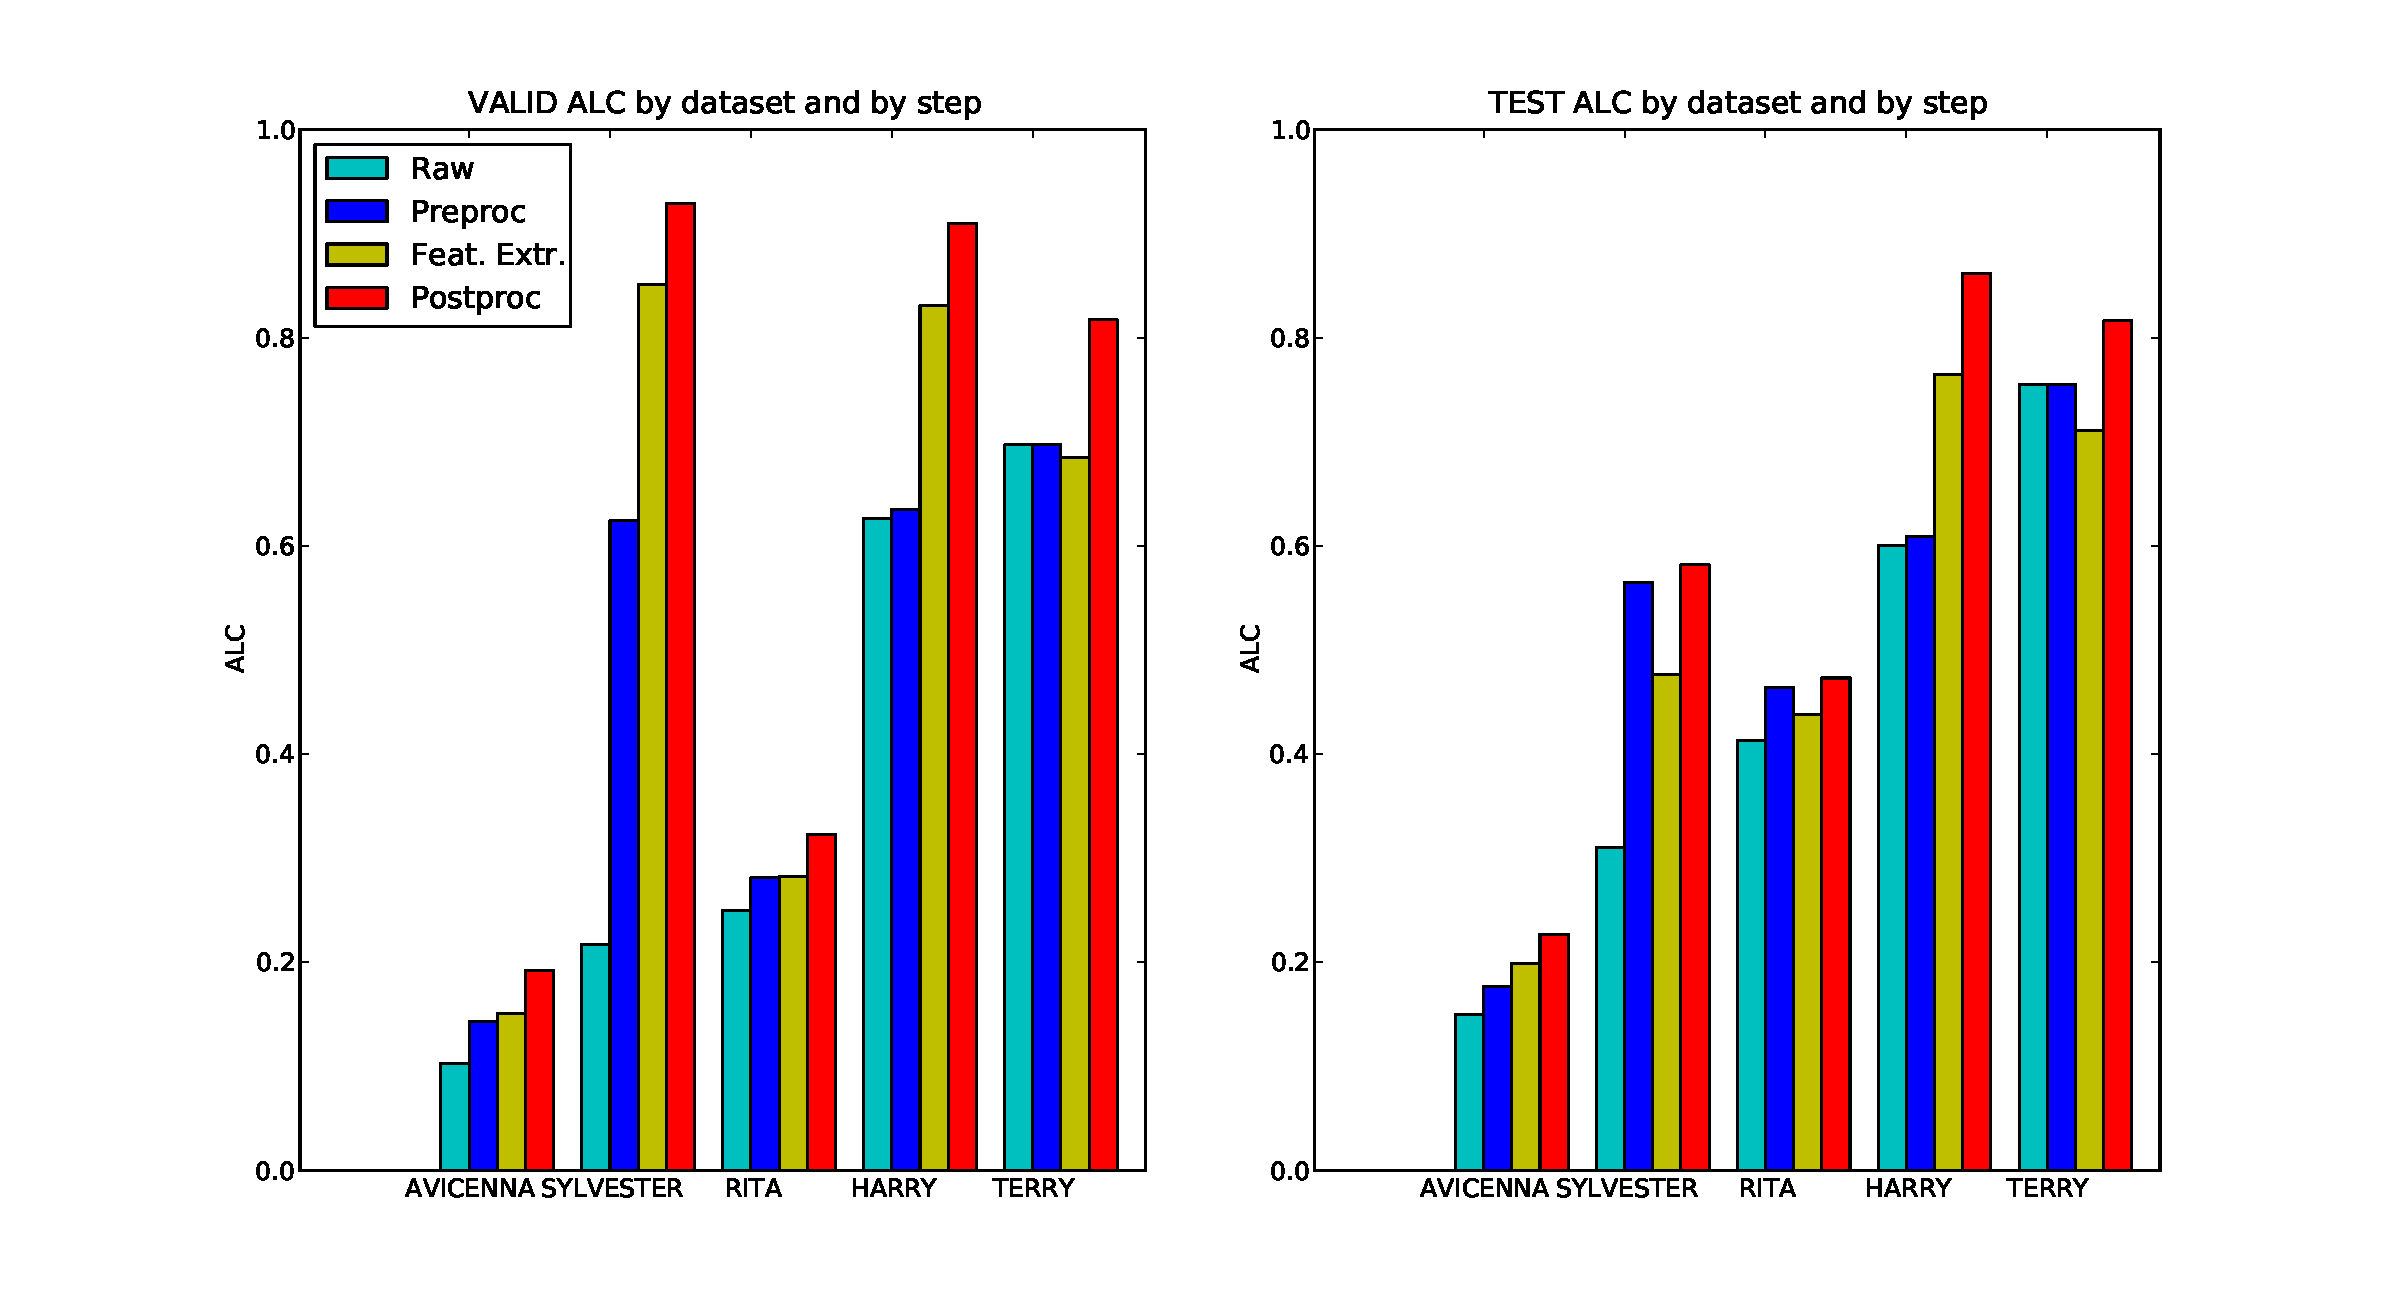
\includegraphics[width=1.\linewidth]{article1/images/5steps.pdf}
    \caption{\label{fig:charts} For each data set, we report the Validation and Test ALC after each layer (from raw data to postprocessing). It allows us to see where overfitting arose ({\bf SYLVESTER}) and which of the layers resulted the more important to improve the overall performance.}
    \vspace{-0.2in}
  \end{center}
 \vspace*{-1mm}
\end{figure}


 
\subsection{AVICENNA}
% Gregoire preproc pca whitened 75 comp DAE binomial 0.3 noise nhidden 600
% transductive pca  7

\paragraph{Nature of the data}
It corresponds to arabic manuscripts and consists of $150,205$ training samples of dimension $120$.

\paragraph{Best Architecture}
For preprocessing, we fitted a whitened-PCA on the raw data and kept the first
$75$ components in order to eliminate the noise from the input distribution.
Then, the second layer consisted in a Denoising Autoencoder of $600$ hidden
units trained with a binomial noise, i.e, each component of the input had a
probability $p=0.3$ of being masked (set to 0). The top layer was a transductive PCA 
with only the $7$ principal components.

\paragraph{Results}
This strategy ranked first with a validation and final ALC score of $0.1932$
and $0.2273$ respectively. Training a contractive auto-encoder gives similar
results on the validation set i.e a validation and final ALC score of $0.1930$
and $0.1973$ respectively.
% EL: For the next 3 experiments, I kept the personal tone ('we ...').  I can
% rewrite it to a neutral tone if it is not appropriate.  Also, the present
% tense is used.  The fourth experiment use the past tense.  I can rewrite
% those three to past tense to make it more uniform.
\subsection{HARRY}



\paragraph{Nature of the data} It corresponds to human actions and consists of
$69,652$ training samples of dimension $5,000$, which are
sparse: only $~2\%$ of the components
are typically non-zero.

\paragraph{Best Architecture} For the first layer, we uniformized the non-zero
feature values (aggregating all features)
across the concatenation of the training, validation and test
sets.  For the second layer, we trained on the union of the 3 sets a Denoising
Auto-Encoder with rectifier units and reconstruction sampling. We used the
binomial masking noise $(p=0.5)$ as corruption process, the logistic sigmoid as
reconstruction activation function and the cross entropy as reconstruction
error criterion.  The size of the hidden layer was $5000$ 
% as the input
and we added an $L_1$ penalty on the activation values to encourage sparsity of
the representation. For the third layer, we applied a transductive PCA and kept
$3$ components.

\paragraph{Results} We obtained the best validation ALC score of the
competition.  This was also the case for the final evaluation score with an ALC
score of 0.861933, whereas the second best obtained 0.754497.
Figure~\ref{fig:harry} shows the final data representation we obtained for the
test (evaluation) set. 
%     after the transductive PCA.

\begin{figure}[t]
  \begin{center}
    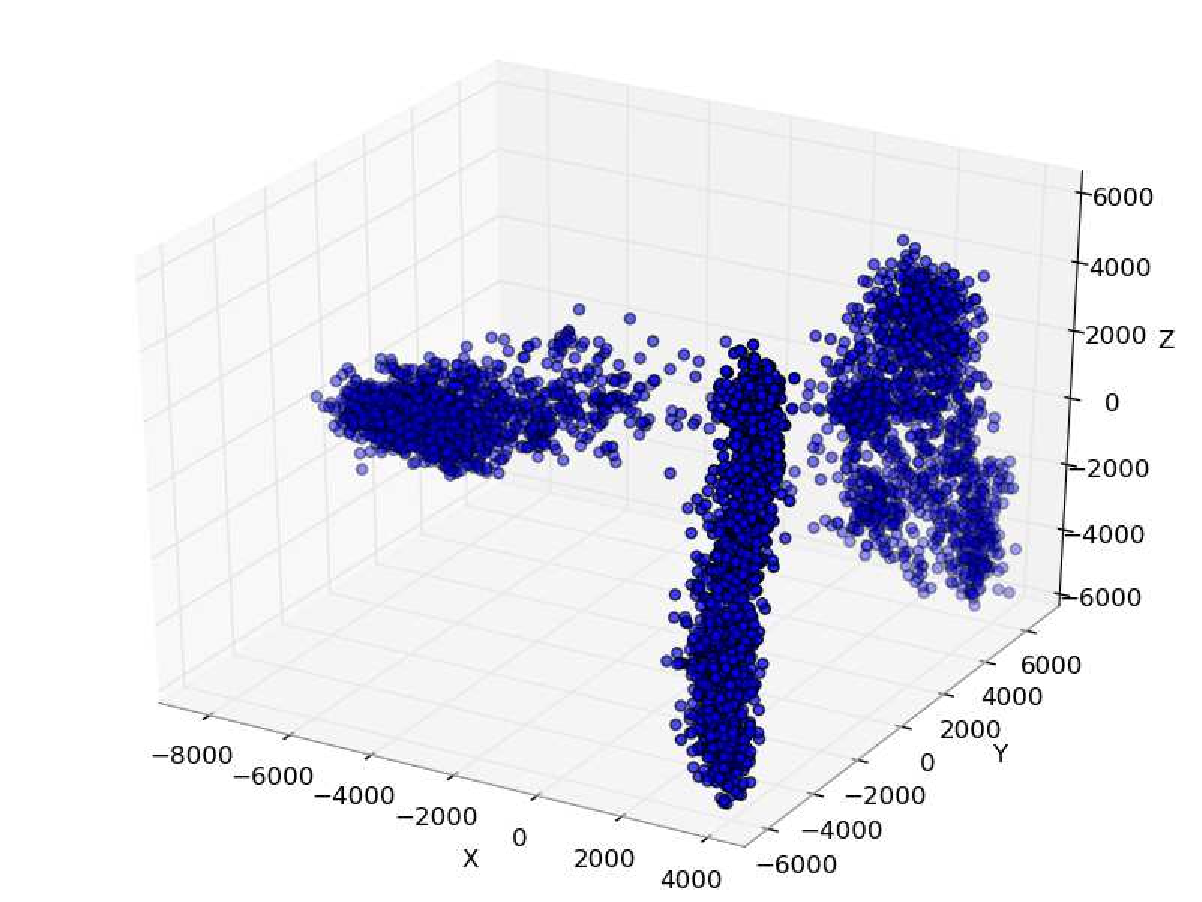
\includegraphics[width=0.75\linewidth]{article1/images/harry_cluster.pdf}
    \caption{\label{fig:harry}  {\bf HARRY} evaluation set 
     after the transductive PCA, the data is nicely clustered, suggesting
     that the learned preprocessing has discovered the underlying class structure.}
    \vspace{-0.2in}
  \end{center}
 \vspace*{-1mm}
\end{figure}


\subsection{TERRY}
% Xavier


\paragraph{Nature of the data} This is a natural language processing
(NLP) task, with $217,034$ training samples of dimension $41,236$, and
a high level of sparsity: only $~1\%$ of the components are non-zero in average.


\paragraph{Best Architecture}

A setup similar to {\bf HARRY} has been used for {\bf TERRY}.  For the first layer, we kept
only the features that were active on both training and validation sets (and similarly
with the test set, for preparing the test set representations). Then, we
divided the non-zero feature values by their standard deviation across the
concatenation of the training, validation and test set.  For the
second layer, we trained on the three sets a Denoising Auto-Encoder with rectifier units and
reconstruction sampling.  We used binomial masking noise ($p=0.5$) as
corruption process, the logistic sigmoid as reconstruction activation function
and the squared error as reconstruction error criterion.  The size of the
hidden layer was $5000$ 
%as the input
and we added an $L_1$ penalty on the activation values to encourage sparsity of
the representation.  For the third layer, we applied a transductive PCA and
kept the leading $4$ components.

\paragraph{Results}

We ranked second on this dataset with a validation and final score of
$0.816752$ and $0.816009$.

\subsection{SYLVESTER} 

\paragraph{Nature of the data} It corresponds to ecology data and consists of $572,820$ training samples of dimension $100$.

\paragraph{Best Architecture}


For the first layer, we extracted the meaningful features and discarded the apparent noise
dimensions using PCA. We used the first 8 principal dimensions as the feature
representation produced by the layer because it gave the best performance on
the validation set. We also whitened this new feature representation by dividing
each dimension by its corresponding singular value (square root of the eigenvalue
of the covariance matrix, or corresponding standard deviation of the component). 
Whitening gives each dimension
equal importance both for the classifier and subsequent feature extractors.
For the second and third layers, we used a Contractive Auto-Encoder (CAE).  We
have selected a layer size of 6 based on validation ALC.
For the fourth layer, we again apply a transductive PCA.

\iffalse
\caption{Validation performance increases with the depth of our feature
hierarchy for the {\bf SYLVESTER} dataset. ALC: Raw Data ($0.2167$), $1$st Layer ($0.6238$), $2$nd Layer ($0.7878$), $3$rd Layer ($0.8511$), t-PCA($0.9316$)} \label{fig:sylvester} \end{figure*}
%\subsubsection{Phase 1}
\fi


\begin{figure}
\centering
\begin{subfigure}{.3\textwidth}
\centering
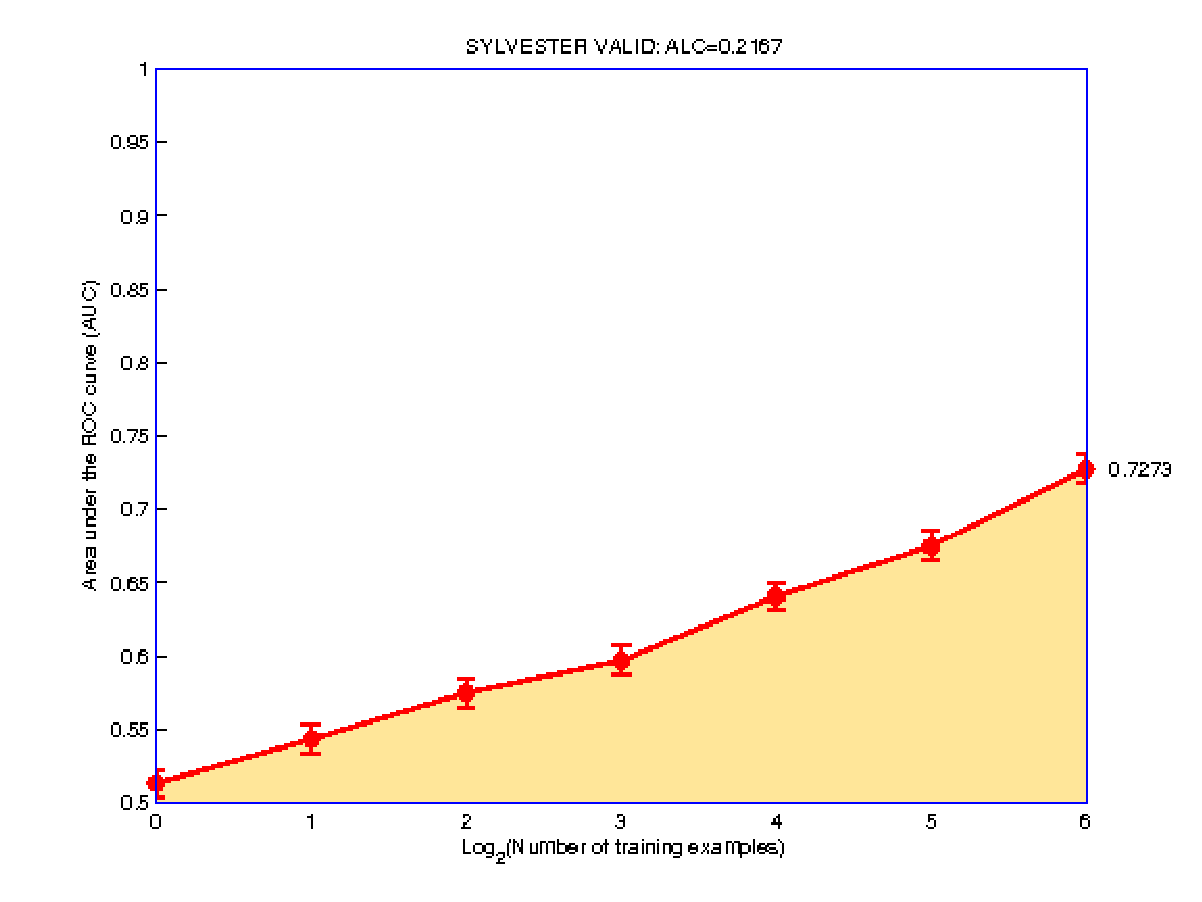
\includegraphics[height=0.15\textheight,keepaspectratio]{article1/images/syl4.pdf}
\caption{Raw Data}
\end{subfigure}
\begin{subfigure}{.3\textwidth}
\centering
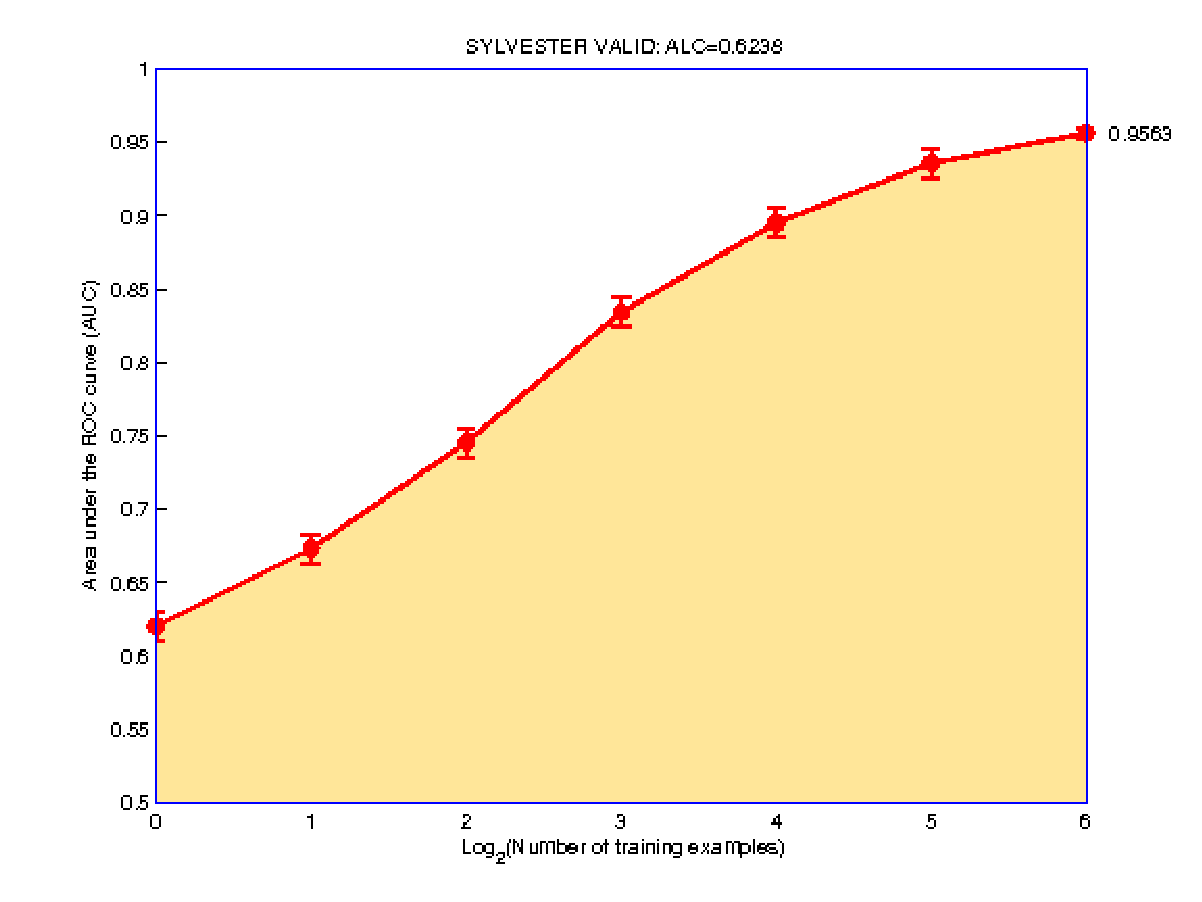
\includegraphics[height=0.15\textheight,keepaspectratio]{article1/images/syl0.pdf}
\caption{1st layer}
\end{subfigure}
\begin{subfigure}{.3\textwidth}
\centering
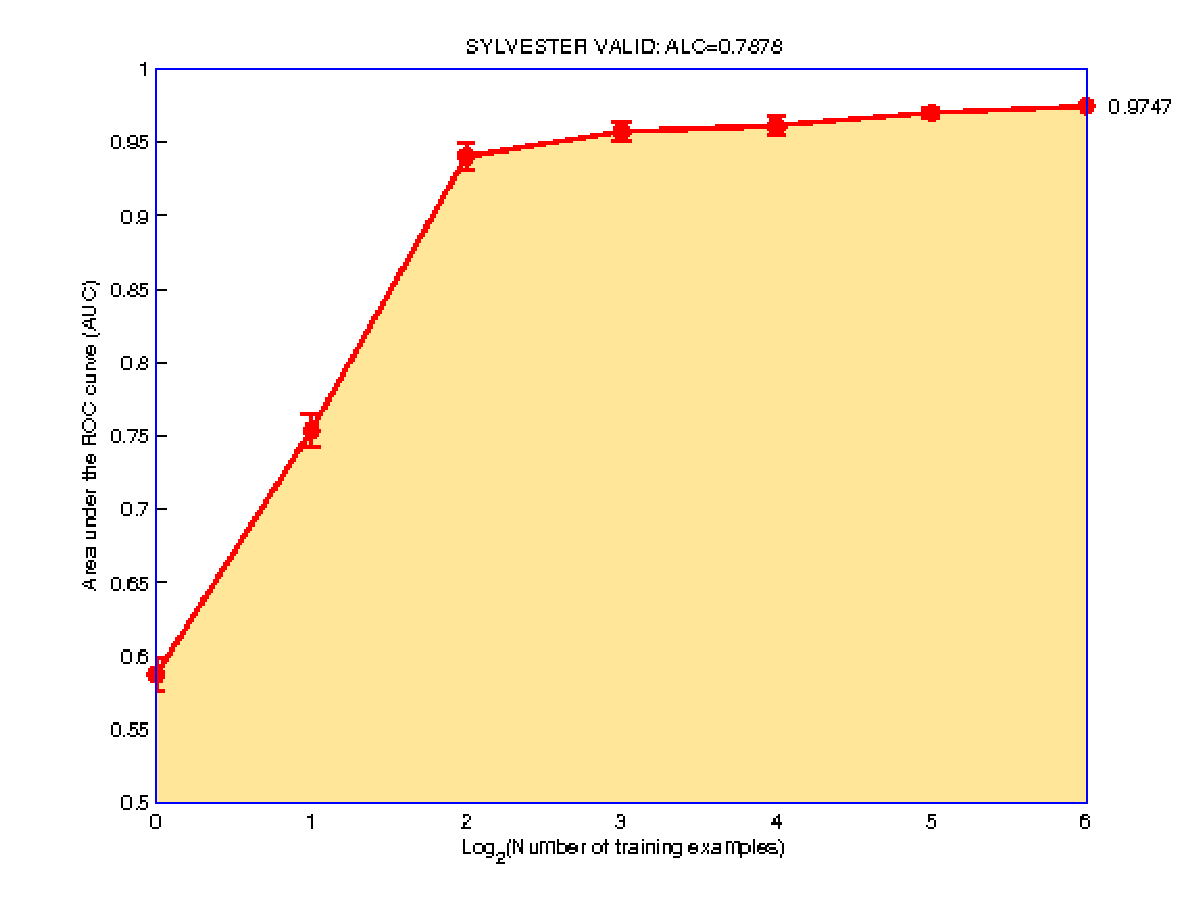
\includegraphics[height=0.15\textheight,keepaspectratio]{article1/images/syl1.pdf}
\caption{2nd layer}
\end{subfigure}\\

\begin{subfigure}{.3\textwidth}
\centering
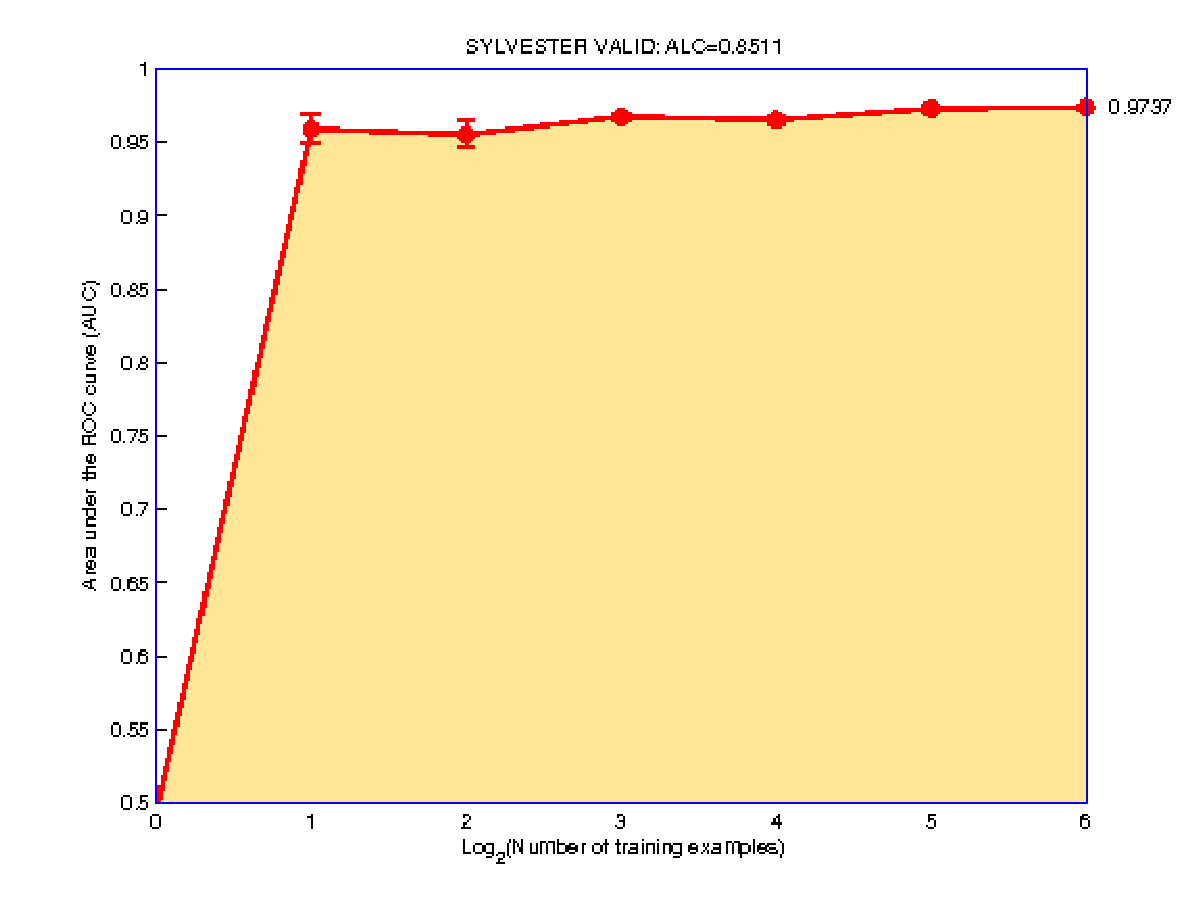
\includegraphics[height=0.15\textheight,keepaspectratio]{article1/images/syl2.pdf}
\caption{3rd layer}
\end{subfigure}
\begin{subfigure}{.3\textwidth}
\centering
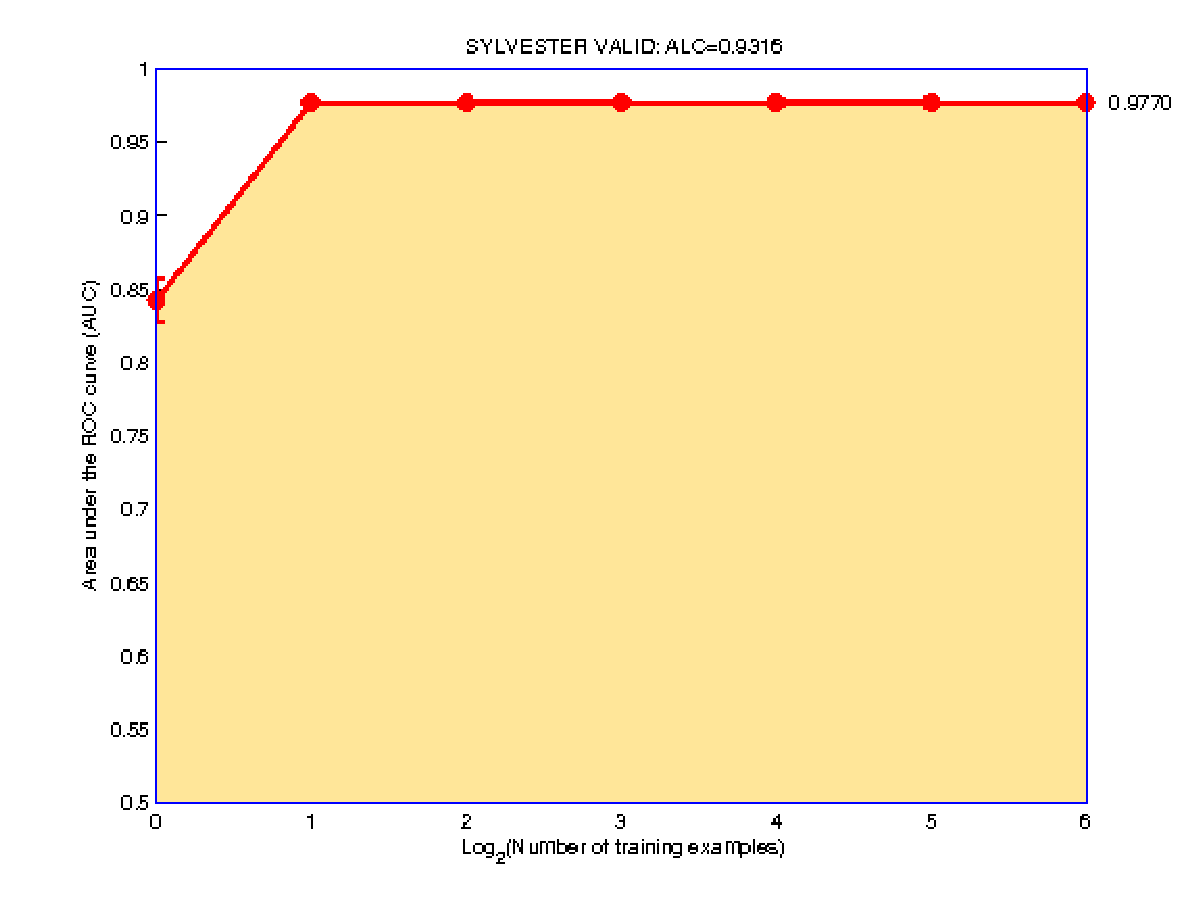
\includegraphics[height=0.15\textheight,keepaspectratio]{article1/images/syl3.pdf}
\caption{t-PCA}
\end{subfigure}
\caption{Validation performance increases with the depth of our feature
hierarchy for the {\bf SYLVESTER} dataset. ALC: Raw Data ($0.2167$), $1$st
Layer ($0.6238$), $2$nd Layer ($0.7878$), $3$rd Layer ($0.8511$),
t-PCA($0.9316$)}
\label{fig:sylvester}
\end{figure}




Figure \ref{fig:sylvester} shows the evolution of the ALC curve for each layer of the
hierarchy.  Note that at each layer, we only use the top-level features as the
representation.

\paragraph{Results}

This yielded an ALC of $0.85109$ for the validation set and $0.476341$ for the test set.
The difference in ALC may be explained by the fact that Sylvester is the only dataset where
the test set contains more classes than the validation set and, and thus our
assumpptions of equal number of classes might have hurt test performance here.

%\subsubsection{Phase 2}
%We tackled the problem of transduction by creating a better validation criterion. Using the
%criterion described in section \ref{sec:criterion}, we found that a simple Principal
%Component Analysis (PCA) with 8 principal components yielded the best transduction for this
%dataset.

\subsection{RITA}
% EL: The writting style is was really different from the others and it seems
%     the specificity of the u-ssRBM requires more explanation, I leave it to you 
%     Greg to decide whether to rewrite it or not!

% G: Guillaume j'ai tente d'uniformiser ta description avec les autres
% en esperant que ça t'aille


\paragraph{Nature of the data} It corresponds to the CIFAR RGB image dataset and consists of $111,808$ training samples of dimension $7,200$.

\paragraph{Best Architecture}



The $\mu$-ssRBM was initially developed as a model for natural images. As such,
it was a natural fit for the {\bf RITA} dataset. Their ability to learn the pooling
structure was also a clear advantage, since the max-pooling strategy typically
used in vision tasks with convolutional networks~\citep{LeCun98-small} could no longer be employed due to the
obfuscated nature of the dataset.
% The main factors which were considered for
%this series of experiments were: the choice of preprocessing, the
%number of hidden units, the learning rate and number of training epochs,
%the pooling factor $K$ and finally the post-processing.

%Since the likelihood is intractable for large RBMs, one usually relies on a
%proxy (such as classification error) to choose the hyper-parameters. Without
%having access to the labels however, we proceeded as follows.

For pre-processing, each image has been contrast-normalized. Then, we reduced the
dimensionality of the training dataset by learning on the first $1,000$
principal components. For feature extraction, we chose the number of hidden
units to be large enough ($1000$) while still being computationally efficient on GPUs.
The learning rate of $10^{-3}$ and number of training updates ($110,000$
updates with minibatches of size $16$) are chosen such that hidden units have
sparse activations through pools of size $9$, hovering around $10$-$25\%$.
% Finally, we tried $K \in
%\{2,9,50\}$ and uploaded all three representations (after post-processing) to
%the UTLC server. We chose $K=9$ as it gave the best results on the validation
%set.
The post-processing was consistent with the other datasets: we used the
transductive PCA method using only the first $4$ principal components.

\paragraph{Results}

This yielded an ALC score of $0.286$ and $0.437$ for the validation and final
test sets respectively. We also tried to stack $3$ layers of contractive
auto-encoders directly on the raw data and it achieved a valid ALC of
$0.3268$. As it appeared actually transductive, we prefered to keep the
$\mu$-ssRBM in our competition entries because it was trained on the whole
training set.


\section{Conclusion}

The competition setting with different class labels in the validation and the test sets
was quite unusual. The similarity between two classes must be sufficient for
transfer learning to be possible.  %However, similarity is currently assessed
%through human intuition rather than a well defined mathematical property of
%the different classes. 
More formal assessments of class similarity might be useful in such settings.
It is not obvious that the similarity between the
subsets of classes chosen for the different datasets in the context of the
competition is sufficient for an effective generalization, neither that the
similarity between the subsets of classes found in the transfer labels is
representative of the similarity between the classes found in the training, validation
and test datasets.  Finally, for assessing transfer across classes properly
would require a larger number of classes. 
In a future competition, we suggest that both similarity
and representativeness (including number of classes)
should be ensured in a more formal or empirical way.

On all five tasks, we have found the idea of stacking different layer-wise
representation-learning algorithms to work very well. One surprise was the
effectiveness of PCA both as a first layer and a last layer, in a transductive
setting. As core feature-learning blocks, the contractive auto-encoder, the
denoising auto-encoder and spike-and-slab RBM worked best for us on the dense
datasets, while the sparse rectifier denoising auto-encoder worked best on the
sparse datasets.

%\bibliography{strings,ml,aigaion}

\section*{Acknowledgements}

The authors acknowledge the support of the following agencies for research
funding and computing support: NSERC, RQCHP, CIFAR. This is also funded in part by
the French ANR Project ASAP ANR-09-EMER-001.


%{%\small
%\bibliography{strings,ml,aigaion,aaron} %,how_we_won}
%\bibliographystyle{plain}
%\bibliographystyle{natbib}
%}

%\end{document}

\chapter{Pr\'{e}ambule au Deuxi\`{e}me Article }

\section{D\'{e}tails de l'article}

{ \bf Unsupervised Learning of Semantics of Object Detections for Scene
Categorization} Gr\'{e}goire Mesnil, Salah Rifai, Antoine Bordes, Xavier
Glorot, Yoshua Bengio and Pascal Vincent.  { \it Advances in Intelligent
Systems, Computing} Springer, Vol.  318, Maria De Marsico and Ana Fred (Eds):
Pattern Recognition Applications and Methods, 2015\\ 

{\it Contribution Personnelle} Le d\'{e}but de ce travail a \'{e}t\'{e}
effectu\'{e} en collaboration avec Antoine Bordes, Xavier Glorot et Salah
Rifai. L'id\'{e}e initiale \'{e}tait d'utiliser le contexte dans des images
(pr\'{e}sence d'objets) pour am\'{e}liorer la cat\'{e}gorisation de sc\`{e}nes.
Je me suis charg\'{e} de pr\'{e}parer les repr\'{e}sentations d'Object Bank
pour tous nos datasets et j'ai effectu\'{e} l'int\'{e}gralit\'{e} des
exp\'{e}riences except\'{e} celles relatives aux CAEs r\'{e}alis\'{e}es par
Salah Rifai. J'ai ensuite adapt\'{e} le pipeline de la comp\'{e}tition afin de
r\'{e}duire la dimension d'entr\'{e}e et permettre un apprentissage non
supervis\'{e}.  Apr\`{e}s plusieurs discussions fructueuses lors
d'une pr\'{e}sentation \`{a} un workshop de NIPS en 2011
\citep{Mesnil-workshop-nips}, l'id\'{e}e s'est am\'{e}lior\'{e}e et notre
publication \citep{Mesnil-icpram} a \'{e}t\'{e} accept\'{e}e \`{a} ICPRAM.
Apr\`{e}s l'oral, le papier a \'{e}t\'{e} selectionn\'{e} pour publication dans
un recueil contenant les meilleurs papiers pr\'{e}sent\'{e}s \`{a} cette
conf\'{e}rence \citep{Mesnil-icpram-journal}. J'ai r\'{e}dig\'{e} l'article en
collaboration avec les co-auteurs.

\section{Contexte}

\`{A} cette \'{e}poque les r\'{e}seaux de neurones convolutionnels n'ont pas
encore remport\'{e} la comp\'{e}tition ImageNet \citep{Krizhevsky-2012-small} et les
d\'{e}tecteurs d'objet \`{a} l'\'{e}tat de l'art restent ceux utilisés dans
Object Bank \citep{lsvm-pami}. Pour la classification de sc\`{e}nes, Object
Bank est encore la m\'{e}thode \`{a} l'\'{e}tat de l'art.  C'est pourquoi nous
avons d\'{e}cid\'{e} d'utiliser les repr\'{e}sentations d'Object Bank comme
support \`{a} notre travail afin d'explorer si une combinaison des
d\'{e}tections d'objets de mani\`{e}re plus abstraite permettait un gain en
performance.

\section{Contributions}

Malgre ses tr\`{e}s bonnes performances \`{a} l'\'{e}poque, un des
inconv\'{e}nients d'Object Bank reste la dimensionnalit\'{e} tr\`{e}s
\'{e}lev\'{e}e de la repr\'{e}sentation.  Dans notre travail, nous avons
explor\'{e} diff\'{e}rentes techniques pour combiner les d\'{e}tections
d'objets afin de permettre aux chercheurs int\'{e}ress\'{e}s d'utiliser une
repr\'{e}sentation d'Object Bank plus compacte et plus performante.


\section{R\'{e}cents d\'{e}veloppements}

Il est certain qu'utiliser des d\'{e}tecteurs d'objets \`{a} base de
r\'{e}seaux de neurones convolutionnels am\'{e}liorerait nettement les
performances de notre approche \citep{Scene-14}.  Au moment du
d\'{e}veloppement de ces id\'{e}es, notre m\'{e}thode souffrait principalement
du manque de pr\'{e}cision des d\'{e}tecteurs d'objets. 


%%%%%%%%%%%%%%%%%%%%%%% file typeinst.tex %%%%%%%%%%%%%%%%%%%%%%%%%
%
% This is the LaTeX source for the instructions to authors using
% the LaTeX document class 'llncs.cls' for contributions to
% the Lecture Notes in Computer Sciences series.
% http://www.springer.com/lncs       Springer Heidelberg 2006/05/04
%
% It may be used as a template for your own input - copy it
% to a new file with a new name and use it as the basis
% for your article.
%
% NB: the document class 'llncs' has its own and detailed documentation, see
% ftp://ftp.springer.de/data/pubftp/pub/tex/latex/llncs/latex2e/llncsdoc.pdf
%
%%%%%%%%%%%%%%%%%%%%%%%%%%%%%%%%%%%%%%%%%%%%%%%%%%%%%%%%%%%%%%%%%%%

\iffalse
\documentclass[runningheads,a4paper]{llncs}

\usepackage{amssymb}
\setcounter{tocdepth}{3}
\usepackage{graphicx}

\usepackage{url}
\usepackage{color}

\urldef{\mailsa}\path|{alfred.hofmann, ursula.barth, ingrid.haas, frank.holzwarth,|
\urldef{\mailsb}\path|anna.kramer, leonie.kunz, christine.reiss, nicole.sator,|
\urldef{\mailsc}\path|erika.siebert-cole, peter.strasser, lncs}@springer.com|    
\newcommand{\keywords}[1]{\par\addvspace\baselineskip
\noindent\keywordname\enspace\ignorespaces#1}

\newcommand{\acom[1]}{\textcolor{red}{#1}}


\begin{document}

\mainmatter  % start of an individual contribution

% first the title is needed


% a short form should be given in case it is too long for the running head
\titlerunning{Object Detections' Semantics for Scene Categorization}

% the name(s) of the author(s) follow(s) next
%
% NB: Chinese authors should write their first names(s) in front of
% their surnames. This ensures that the names appear correctly in
% the running heads and the author index.
%

\author{   
% Gregoire Salah Antoine Xavier Yoshua Pascal
Gr\'{e}goire Mesnil$^{1,2}$ \and Salah Rifai$^{1}$
\and Antoine Bordes$^{3}$ \and Xavier Glorot$^{1}$\and\\
Yoshua Bengio$^{1}$ \and Pascal Vincent$^{1}$
}
%\affiliation{\sup{1}LISA, Universit\'{e} de Montr\'{e}al, Qu\'{e}bec, Canada}
%\affiliation{\sup{2}LITIS, Universit\'{e} de Rouen, France}
%\affiliation{\sup{3}CNRS - Heudiasyc UMR 7253, Universit\'{e} de Technologie de Compi\`{e}gne, France}
%\email{gregoire.mesnil@umontreal.ca}
%}


%\author{Alfred Hofmann%
%\thanks{Please note that the LNCS Editorial assumes that all authors have used
%the western naming convention, with given names preceding surnames. This determines
%the structure of the names in the running heads and the author index.}%
%\and Ursula Barth\and Ingrid Haas\and Frank Holzwarth\and\\
%Anna Kramer\and Leonie Kunz\and Christine Rei\ss\and\\
%Nicole Sator\and Erika Siebert-Cole\and Peter Stra\ss er}
%
\authorrunning{Gr\'egoire Mesnil et al.}
% (feature abused for this document to repeat the title also on left hand pages)

% the affiliations are given next; don't give your e-mail address
% unless you accept that it will be published
\institute{
%Springer-Verlag, Computer Science Editorial,\\
%Tiergartenstr. 17, 69121 Heidelberg, Germany\\
%\mailsa\\
%\mailsb\\
%\mailsc\\
%\url{http://www.springer.com/lncs}}
$^{1}$ LISA, Universit\'{e} de Montr\'{e}al, Qu\'{e}bec, Canada\\
$^{2}$ LITIS, Universit\'{e} de Rouen, France\\
$^{3}$ CNRS - Heudiasyc UMR 7253, Universit\'{e} de Technologie de Compi\`{e}gne, France
%
}
%
% NB: a more complex sample for affiliations and the mapping to the
% corresponding authors can be found in the file "llncs.dem"
% (search for the string "\mainmatter" where a contribution starts).
% "llncs.dem" accompanies the document class "llncs.cls".
%

%\toctitle{Lecture Notes in Computer Science}
%\tocauthor{Authors' Instructions}
\maketitle


\begin{abstract} Classifying scenes (e.g. into ``street'', ``home'' or
``leisure'') is an important but complicated task nowadays, because images come
with variability, ambiguity, and a wide range of illumination or scale
conditions.
  %
  Standard approaches build an intermediate representation of the global image
  and learn classifiers on it. %~\cite{Lazebnik06,Lowe99,Csurka04}.
  %
  Recently, it has been proposed to depict an image as an aggregation of its
  contained objects:~ the representation on which classifiers are trained is
  composed of many heterogeneous feature vectors derived from various object
  detectors.
  %
  In this paper, we propose to study different approaches to efficiently learn
  contextual semantics out of these object detections.
  %
  We use the features provided by Object-Bank~\cite{LiJiaLi10} (177 different
  object detectors producing 252 attributes each), and show on several
  benchmarks for scene categorization that careful combinations, taking into
  account the structure of the data, allows to greatly improve over original
  results (from $+5\%$ to $+11\%$)
  %of the original paper (+11\% on MIT Indoor, +5\% on UIUC Sports and +4\% on
  %15-scenes) 
  while drastically reducing the dimensionality of the % Object-Bank
      representation by 97\% (from $44,604$ to $1,000$).
  %
  We also show that the uncertainty relative to object detectors hampers the
  use of external semantic knowledge to improve detectors combination, unlike
  our unsupervised learning approach.

\keywords{Unsupervised Learning, Transfer Learning, Deep Learning, Scene Categorization, Object Detection}
\end{abstract}
\fi

\chapter{Unsupervised Learning of Semantics of Object Detections for Scene Categorization}
\section{Introduction}


Automatic scene categorization is crucial for many applications such
as content-based image indexing \cite{Smeulders:2000} or image
understanding.
%
This is defined as the task of assigning images to predefined
categories ( ``office'', ``sailing'', ``mountain'', etc.).
%
Classifying scene is complicated because of the large variability of
quality, subject and conditions of natural images which lead to many
ambiguities w.r.t. the corresponding scene label.

Standard methods build an intermediate representation before
classifying scenes by considering the image as a whole
\cite{Torralba03,Vogel:2004,FeiFei:2005,Oliva06}. In particular, many
such approaches rely on power spectral information, such as
magnitude of spatial frequencies \cite{Oliva06} or local texture
descriptors \cite{FeiFei:2005}.
%
They have shown to perform well in cases where there are large
numbers of scene categories.

Another line of work conveys promising potential in scene categorization.
%
First applied to object recognition~\cite{Farhadi:2009}, attribute-based
methods have now proved to be effective for dealing with complex scenes.
%
These models define high-level representations by combining semantic
lower-level elements, e.g., detection of object parts.
%
A precursor of this tendency for scenes was an adaptation of
pLSA~\cite{Hofmann:2001} to deal with ``visual words'' proposed by
\cite{Bosh:2006}. 
%
An extension of this idea consists in modeling an image based on its content
i.e. its objects \cite{Espinace10ICRA,LiJiaLi10}. Hence, the Object-Bank (OB)
project~\cite{LiSuLimFeiFei} aims at building high-dimensional over-complete
representations of scenes (of dimension $44,604$) by combining the outputs of
many object detectors ($177$) taken at various poses, scales and positions in
the original image (leading to $252$ attributes per detector).
% I added poses which correspond to root filters G To unify language pose or
% root = pose detector or object = object
%
Experimental results indicate that this approach is effective since simple
classifiers such as Support Vector Machines trained on their representations
achieve state-of-the-art performance.
%
However, this approach suffers from two flaws: (1) curse of dimensionality
(very large number of features) and (2) individual object detectors have a poor
precision (30\% at most).
%
%Solving (2) is beyond the scope of this work.
%
To solve (1), the original paper proposes to use structured norms and group
sparsity to make best use of the large input.
%
%Such good results are simply obtained by learning the classifier on the plain
%concatenation of the attributes extracted by each object detector.
%
Our work studies new ways to combine the very rich information provided by
these multiple detectors, dealing with the uncertainty of the detections.
%
A method designed to select and combine the most informative attributes would
be able to carefully manage redundancy, noise and structure in the data,
leading to better scene categorization performance.


%% NEW STUFF

Hence, in the following, we propose 
%two kinds of strategies 
a sequential $2$-steps strategy for combining the feature representations
provided by the OB object detectors on which the linear SVM classifier is
destined to be trained for categorizing scenes.
%
The first step adapts Principal Components Analysis (PCA) to this particular
setting: we show that it is crucial to take into account the structure of the
data in order for PCA to perform well.
%
The second one is based on {\em Deep Learning}.
%
Deep Learning has emerged recently (see \cite{Bengio-2009} for a review) and is
based on neural network algorithms able to discover data representations in an
unsupervised
fashion~\cite{Hinton06,Bengio-nips-2006-short,ranzato-07-small,Koray-08,Jarrett-ICCV2009}.
%
We propose to use this ability to combine multiple detector features. Hence, we
present 
%several models trained in a parallel fashion 
a model trained using Contractive Auto-Encoders
\cite{Rifai+al-2011,Salah+al-2011}, which have already proved to be efficient
on many image tasks and has contributed to winning a transfer learning
challenge~\cite{UTLC+LISA-2011}.
% Plutot dans le cas general que sur des images tasks non ? on s'attaque a des
% features sans connaissance apriori comme on pourrait l'avoir pour des images
% Gregoire
%
% Antoine: peut-être mais ici il faut justifier pourquoi on utilise des CAE et
% pas des RBM ou des DAE -- une raison peut être leur efficacité sur des images
%
%Object-Bank detector outputs (of dimension $252$) and transforms it
%non-linearly into a smaller vector (of dimension $100$). The second layer
%combines these $177$ compressed feature vectors into a unified representation
%(of dimension $1000$?). 
%% CAE

%Exp
We validate the quality of our models in an extensive set of experiments in
which several setups of the sequential feature extraction process are evaluated
on benchmarks for scene classification
\cite{Lazebnik06,LiJiaLi07,Quattoni09,Xiao:2010}. 
%
 We show that our best results substantially outperform the original methods
 developed on top of OB features, while producing representations of much lower
 dimension.
  %
  The performance gap is usually large, indicating that advanced combinations
  are highly beneficial. 
  % 
  We show that our method based on dimensionality reduction followed by deep
  learning offers a flexibility which makes it able to benefit from
  % transductive,
  semi-supervised and transfer learning.
  %
  %We find that the use of supervised fine-tuning outperforms any of the
  %PCA-based strategies tested.
  %
  %The results on different setups are either state-of-the-art (compared with
  %methods using large combinations of features like \cite{Gao10}) or very
  %close to it. 



%
%We conclude with a discussion of the advantages and drawbacks of both
%combination approaches.

%Antoine: to remove if one needs some space
% The paper is organized as follows. Section~\ref{sec:ob} details
% Object-Bank. Section~\ref{sec:feat} describes the building blocks of
% our combination strategies presented in Section~\ref{sec:combi}. Our
% experimental results are in Section~\ref{sec:exp} and the paper ends
% with a conclusion and discussion of future work in Section~\ref{sec:disc}.

\begin{figure*}
\begin{center}
\begin{tabular}{ccc}
  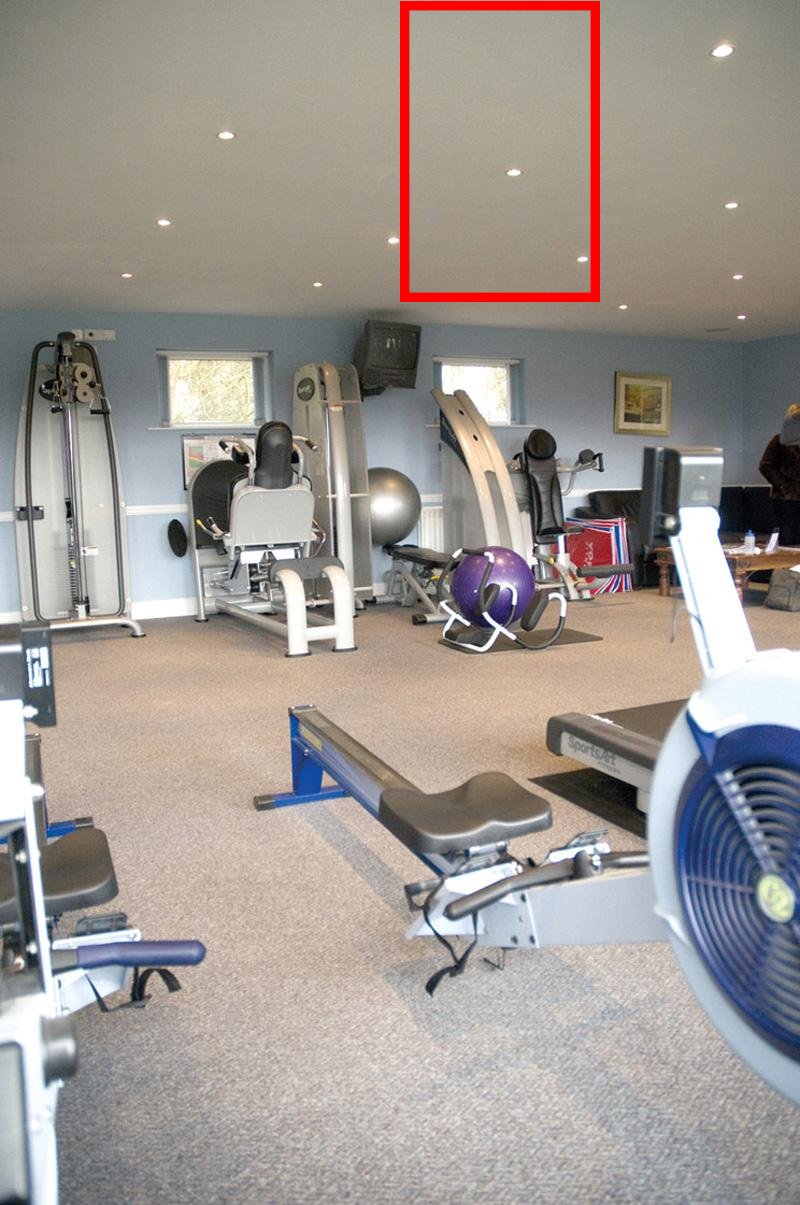
\includegraphics[height=0.20\linewidth]{article2/images/cloud1.png}&
  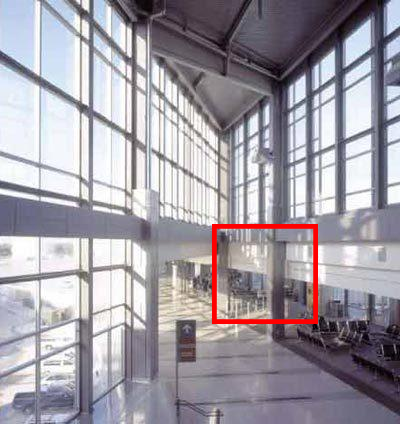
\includegraphics[height=0.20\linewidth]{article2/images/man1.png} &
  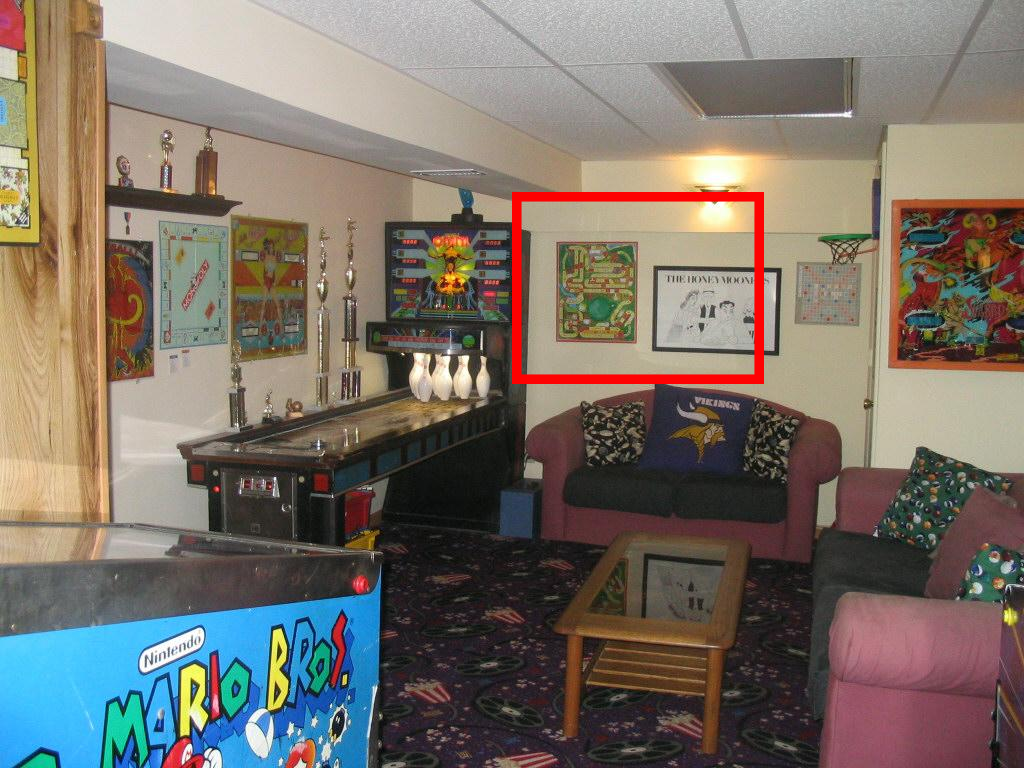
\includegraphics[height=0.20\linewidth]{article2/images/tele1.png}\\ 
  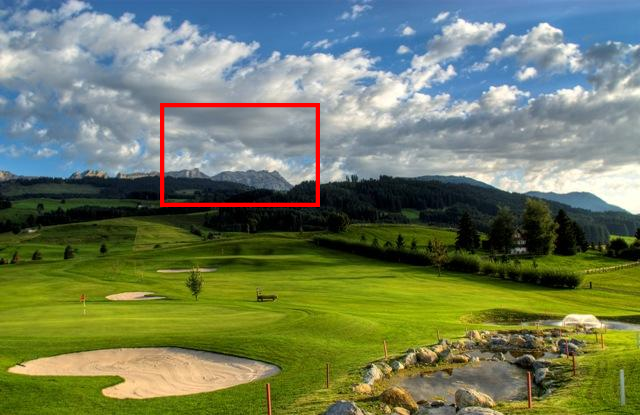
\includegraphics[height=0.20\linewidth]{article2/images/cloud2.png}&
  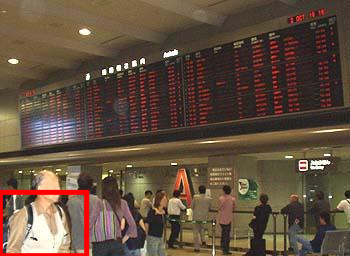
\includegraphics[height=0.20\linewidth]{article2/images/man2.png} &
  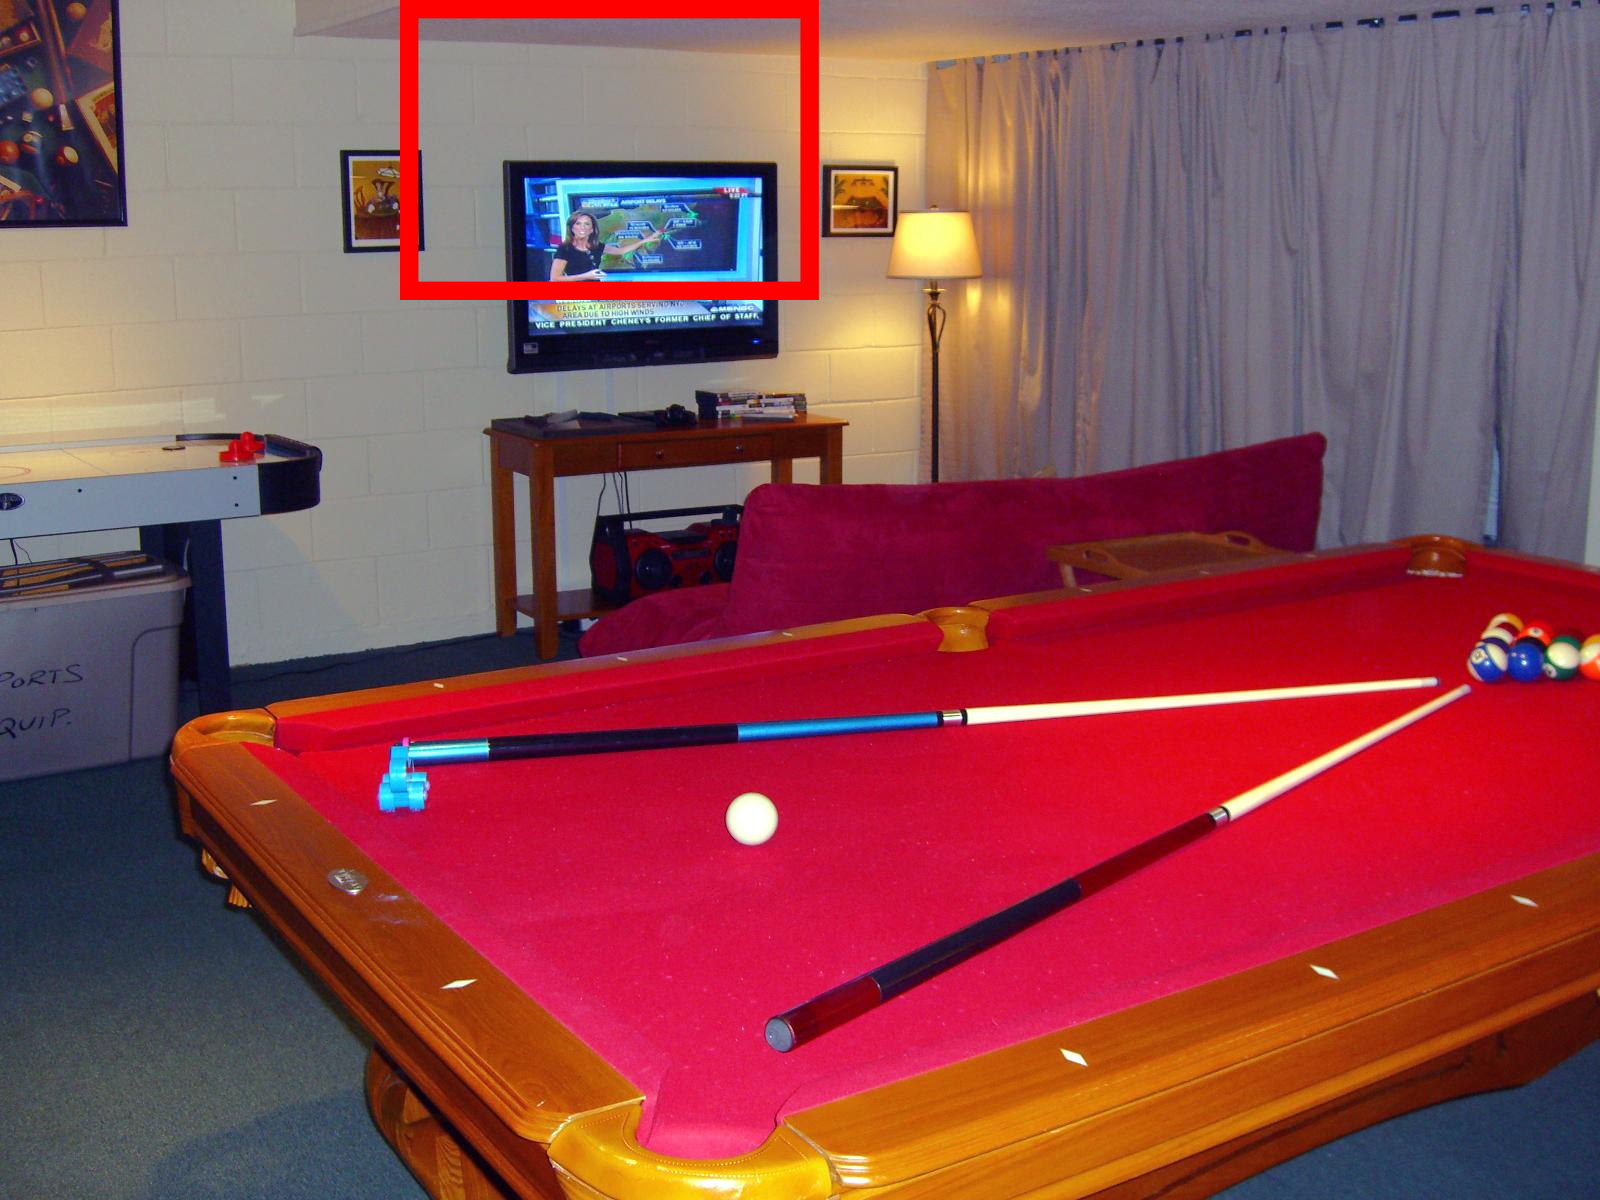
\includegraphics[height=0.20\linewidth]{article2/images/tele2.png}\\ 
\end{tabular}
\end{center}

   \caption{{\it Left:} Cloud {\it Middle:} Man {\it Right:} Television. {\it
   Top:} False Detections {\it Bottom:} True Detections. Images from {\bf
   SUN}~\cite{Xiao:2010} for which we compute the OB representation and display the
   bounding box around the average position of various objects detectors. For
   instance, the \textit{television} detector can be viewed either as a
   \textit{television} detector or a \textit{rectangle} shape detector i.e.
   high-order statistical properties of the image.} \label{fig:images} 
\end{figure*}


%\begin{figure}
%\centering
%\includegraphics[height=6.2cm]{eijkel2}
%\caption{One kernel at $x_s$ (\emph{dotted kernel}) or two kernels at
%$x_i$ and $x_j$ (\textit{left and right}) lead to the same summed estimate
%at $x_s$. This shows a figure consisting of different types of
%lines. Elements of the figure described in the caption should be set in
%italics, in parentheses, as shown in this sample caption.}
%\label{fig:example}
%\end{figure}


\section{Scene Categorization with Object-Bank} \label{sec:ob}

Let us begin by introducing the approach of the OB
project \cite{LiJiaLi10}.
%
First, the $177$ most useful (or frequent) objects were selected from
popular image datasets such as LabelMe \cite{labelme}, ImageNet
\cite{imagenet} and Flickr.
%
For each of these $177$ objects, a specific detector, existing in the
literature \cite{Felzen08,Hoiem05}, was trained.
%
Every detector is composed of $2$ {\em root filters} depending on the
pose, each one coming with its own deformable pattern of parts, e.g., there
is one root filter for the front-view of a bike and one for the
side-view.
%
These $354=177\times 2$ part-based filters (each composed by a root and its parts)
are used to produce features of natural images.
%
For a given image, a filter is convolved at $6$ different scales. At
each scale, the max-response among $21=1+4+16$ positions (whole image,
quadrants, quadrants within each quadrant) is kept, producing a
response map of dimension $126=6\times 21$.
%
All $2\times 177$ maps are finally concatenated to produce an over-complete
representation $x\in\mathbb{R}^{44,604}$ of the original image.
%

In the original OB paper \cite{LiJiaLi10}, classifiers for scene
categorization are learned directly on these feature vectors of
dimension $44,604$.
%
More precisely, $C$ classifiers (Linear SVM or
Logistic Regression) are trained in a $1$-versus-all setting in order to predict the
correct scene category $y_{\textrm{category}}(x)$ among $C$ different
categories.
%
Various strategies using structured sparsity with combinations
  of $\ell_1/\ell_2$ norms have been proposed to handle the
  very large input.

\section{Unsupervised Feature Learning}\label{sec:feat}

% motivation
The approach of OB for the task of scene categorization,
based on specific object detectors, is appealing since it works well
in practice.
%
This suggests that a scene is better recognized by first identifying
basic objects and then exploiting the underlying semantics in the
dependencies between the corresponding detectors.
%

However, it appears that none of the individual object detectors
reaches a recognition precision of more than $30\%$. Hence, one may
question whether the ideal view that inspired this approach (and
expressed above) is indeed the reason of OB's success.
%
Alternatively, one may hypothesize that the $44,604$ OB features are
more useful for scene categorization because they represent high level
statistical properties of images than because they precisely report the 
absence/presence of objects $-$ see Figure~\ref{fig:images}.
%
OB tried structured sparsity to handle this feature selection but there may be
  other ways -- simpler or not.

This paper investigates several ways of learning higher-level features
{\bf on top of} the high dimensional representation provided by OB,
expecting that capturing further structure may improve categorization
performance. Our approach employs \textit{unsupervised feature
  learning/extraction} algorithms, i.e. generic feature extraction
methods which were not developed specifically for images. We will
consider both standard Principal Component Analysis and
Contractive Auto-Encoders
\cite{Rifai+al-2011}. The latter is a recent machine
learning method which has proved to be a robust feature extraction
tool.

\subsection{Principal Component Analysis}

Principal Component Analysis (PCA)~\cite{Pearson-1901,Hotelling1933} 
is the most prevalent technique for
linear dimensionality reduction. A PCA with $k$ components finds the $k$
orthonormal directions of projection in input space that retain most of the
\textit{variance} of the training data. These correspond to the eigenvectors
associated with the leading eigenvalues of the training data's covariance
matrix. Principal components are
ordered, so that the first corresponds to the direction along which the data varies the
most (largest eigenvalue), etc\ldots 

Since we will consider an auto-encoder variant (presented next),
% as an alternative feature extractor to PCA
we should mention here a well-known result: a linear auto-encoder with $k$
hidden units, trained to minimize squared reconstruction error, will learn
projection directions that span the same \textit{subspace} as a $k$ component
PCA~\cite{Baldi89}.  However the regularized non-linear auto-encoder variant
that we consider below is capable of extracting qualitatively different, and
usually more useful, nonlinear features.

\subsection{Contractive Auto-Encoders}

Contractive Auto-Encoders (CAEs) \cite{Rifai+al-2011} are among
the latest developments in a line of machine learning research on nonlinear
feature learning methods, that started with the success of Restricted Boltzmann
Machines~\cite{Hinton06} for pre-training deep networks, and was followed by
other variants of auto-encoders such as
sparse~\cite{ranzato-07-small,Koray-08,Goodfellow2009} and  denoising
auto-encoders~\cite{VincentPLarochelleH2008}.
%,Vincent-JMLR-2010}.  
It was selected here mainly due to its practical ease of use and recent
empirical successes.

Unlike PCA that decomposes the input space into leading {\em global} directions
of variations, the CAE learns features that capture local directions of
variation (in some regions of input space). This is achieved by penalizing the
norm of the Jacobian of a latent representation $h(x)$ with respect to its
input $x$ at training samples. Rifai et al.~\cite{Rifai+al-2011} show that the
resulting features provide a local coordinate system for a low dimensional
manifold of the input space. This corresponds to an atlas of charts, each
corresponding to a different region in input space, associated with a different
set of active latent features. One can think about this as being similar to a
mixture of PCAs, each computed on a different set of training samples that were
grouped together using a similarity criterion (and corresponding to a different
input region), but without using an independent parametrization for each
component of the mixture, i.e., allowing to generalize across the charts, and
away from the training examples.

In the following, we summarize the formulation of the CAE as a regularized
extension of a basic Auto-Encoder (AE). In our experiments, the parametrization
of this AE consists in a non-linear encoder or latent representation $h$ of $m$
hidden units with a linear decoder or reconstruction $g$ towards an input space
of dimension $d$.\\

 Formally, the latent variables
are parametrized by:
\begin{equation}
\label{eq:AE-encoder}
h(x) = s(W x+b_h),
\end{equation}
where $s$ is the element-wise logistic sigmoid
$s(z)=\frac{1}{1+e^{-z}}$, $W\in\mathcal{M}_{m\times d}(\mathbb{R})$ and $b_h\in\mathbb{R}^{m}$ are the parameters to be
learned during training.  Conversely, the units of the decoder are linear
projections of $h(x)$ back into the input space:
\begin{equation}
\label{eq:AE-decoder}
g(h(x)) = W^Th(x).
\end{equation}
Using mean squared error as the reconstruction objective and the
L$2$-norm of the Jacobian of $h$ with respect to $x$ as
regularization, training is carried out by minimizing the following
criterion by stochastic gradient descent:
\begin{eqnarray}
\label{eq:CAE-objective}
\mathcal{J}_{\mathrm{CAE}}(\Theta) = \sum_{x \in {\cal D}} \|x - g(h(x))\|^2 +
\lambda \sum_{i=1}^{m}\sum_{j=1}^{d}\left|\frac{\partial h_{i}}{\partial x_{j}}(x)\right|^2 ,
\end{eqnarray}

where $\Theta=\{ W,b_{h}\}$, ${\cal D}=\{x^{(i)}\}_{i=1,\dots,n}$ corresponds
to a set of $n$ training samples $x\in\mathbb{R}^{d}$ and $\lambda$ is a hyper-parameter
controlling the level of contraction of $h$.
%
A notable difference between CAEs and PCA is that features extracted by CAEs
are non-linear w.r.t. the inputs, so that multiple layers of CAEs can be
usefully composed (stacked), whereas stacking linear PCAs is pointless.

\section{Extracting Better Features with Advanced Combination
  Strategies} \label{sec:combi} %\ref{sec:pwork}


In this work, we study two different sub-structures of OB. We consider
the \textit{pose} response defined by the output of only one part-based filter at all
positions and scales, and the \textit{object} response which is the concatenation of all
\textit{pose} responses associated to an object. Combination
strategies are depicted in Figure~\ref{fig:architectures}.

\subsection{Simplistic Strategies: Mean and Max Pooling}

The idea of pooling responses at different locations
or poses has been successfully used in
Convolutional Neural Networks such as LeNet-$5$
\cite{Lecun99objectrecognition} and other visual processing \cite{Serre05}
architectures inspired by the visual cortex.

Here, we pool the $252$ responses of each object detector into one component
(using the mean or max operator) leading to a representation of size
$177=44604/252$. It corresponds to the mean/max over the object responses at
different scales and locations. One may view the object max responses as
features encoding absence/presence of objects while discarding all the
information about the detector's positions. 



\begin{figure*}
\begin{center}
\begin{tabular}{cccc}
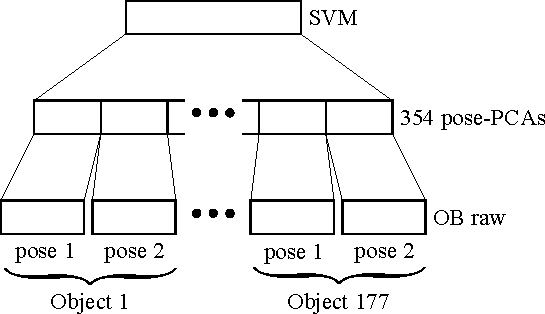
\includegraphics[width=0.33\linewidth]
{article2/images/PosePCAs.pdf}&
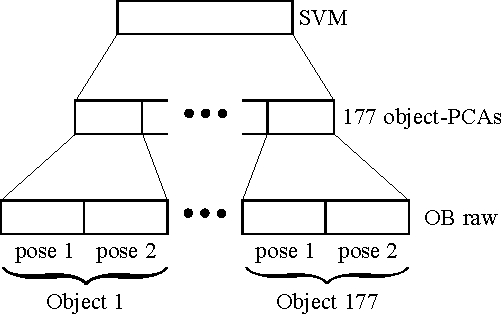
\includegraphics[width=0.33\linewidth]
{article2/images/ObjectPCAs.pdf}&
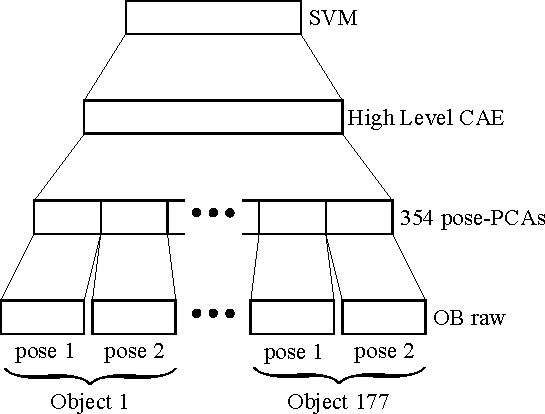
\includegraphics[width=0.33\linewidth]
{article2/images/HighLevelCAE.pdf}\\
\end{tabular}
\end{center}

\caption{{\bf Different Combination Strategies} (a) and (b) \textit{pose} and
\textit{object} PCAs (c) high-level CAE: \textit{pose}-PCA as dimensionality
reduction technique in the first layer and a CAE stacked on top. We denote it
high-level because it can learn \textit{context information} i.e. plausible
joint appearance of different objects.}

\label{fig:architectures}
\end{figure*}

\subsection{Combination Strategies with PCA}

PCA is a standard method for extracting features from high dimensional input, so 
it is a good starting point. However, as we find in our experiments, exploiting
the particular structure of the data, e.g., according to poses, scales, and
locations, can yield to improved results.

\vspace{-0.2cm}
\paragraph{Whole PCA.}
An ordinary PCA is trained on the raw output of OB ($x \in\mathbb{R}^{44,604}$)
without looking for any structure.  Given the high-dimensionality of OB's
representation, we used the Randomized PCA algorithm of the
scikits toolbox\footnote{Available from \textit{http://scikits.appspot.com/}}.


\vspace{-0.2cm} \paragraph{Pose-PCA.} Each of the two \textit{poses} associated
with each \textit{object} detector is considered independently.  This results
in $354=2\times 177$ different PCAs, which  are trained on \textit{pose}
outputs ($x\in\mathbb{R}^{126}$) -- see Figure~\ref{fig:architectures}. 

\vspace{-0.2cm}
\paragraph{Object-PCA.}
Only each \textit{object} response ($x \in\mathbb{R}^{252}$) is considered
separately, therefore $177$ PCAs are trained in total.  It allows the model to
capture variations among all \textit{pose} responses at various scales and
positions -- see Figure~\ref{fig:architectures}.\\ 


Note that, in all cases,  whitening the PCA (i.e. dividing each eigenvector's
response by the corresponding squared root eigenvalue) performs very poorly.
For post-processing, the PCA outputs $\tilde{x}$ are always normalized:
$\tilde{x}\leftarrow (\tilde{x}-\mu)/\sigma $ according to mean $\mu$ and the
deviation $\sigma$ of the whole, per \textit{object} or per \textit{pose} PCA
outputs. Thereby, we ensure contributions from all \textit{objects} or
\textit{poses} to be in the same range.  The number of components in all cases
has been selected according to the classification accuracy estimated by
$5$-fold cross-validation.


\subsection{Improving upon PCA with CAE}

% interesting to capture patterns of variation for one object detector among various scales and size
% 1) variations intra-pose 2) variations among poses,scale and position


% % image -> Hog -> scale (6 scales differents) -> convol (x 2 poses: face et cote) 
% % max pool sur tt image, dans 4 cardants et 16 cadrants. -> 21 positions de
% % candidats max pour 1 scale.

% interesting to capture patterns of variation for one object detector among various scales and size
% 1) variations intra-pose 2) variations among poses,scale and position

% 44604 currently CAE not scaling up to this dim.
% take advantage of struct. (output of 177 obj detectors at different
% poses, scales and positions)

% % 1ere couche:

% % Pour chaque type d'objet/pose, on carcterise les invariances
% % posititon/scale.
% % CAE entraine pour chacune des 177x2 poses sur input 21pos*6scales vers dim 100.
% % (+SVM)

Due to hardware limitations and high-dimensional input, we could not train a
CAE on the whole OB output (``whole CAE''). However, we address this problem 
with the sequential feature extraction steps below.

%\paragraph{High- CAE.}
\label{sec:highlevel}
To overcome the tractability problem that forbids a CAE to be
trained on the whole OB output, we preprocess it by using the
\textit{pose}-PCAs as a dimensionality reduction method. We keep
only the $5$ first components of each \textit{pose}. Given this
low-dimensional representation (of dimension $1,770$), we are able to
train a CAE -- see Figure~\ref{fig:architectures}.
%
The CAE has a global view of all object detectors and
can thus learn to capture {\em context information}, defined by the
joint appearance of combinations of various objects. Moreover, instead
of using an SVM on top of the learned representations, we can use a
Multi-Layer Perceptron whose weights would be initialized by those of
this CAE. This setting is where the CAE has shown to perform
best in practice \cite{Salah+al-2011}.

\section{Experiments} \label{sec:exp}


\subsection{Datasets}


We evaluate our approach on $3$ scene datasets, cluttered indoor images (MIT
Indoor Scene),  natural scenes ($15$-Scenes), and event/activity images
(UIUC-Sports). Images from a large scale scene recognition dataset (SUN-$397$
database) have also been used for unsupervised learning. 
%\vspace{-1ex}
\begin{itemize}
  \item {\bf{MIT Indoor}} is composed of $67$ categories and, following
\cite{LiJiaLi10,Quattoni09}, we used $80$ images from each category for
training and $20$ for testing.

\item {\bf{15-Scenes}} is a dataset of $15$ natural scene
classes. According to \cite{Lazebnik06}, we used $100$ images per class for
training and the rest for testing. 

\item {\bf{UIUC-Sports}} contains $8$ event classes.  We
randomly chose $70$ / $60$ images for our training / test set respectively,
following the setting of \cite{LiJiaLi10,LiJiaLi07}.

\item {\bf{SUN-397}} contains a full variety of $397$  well sampled
scene categories ($100$ samples per class) composed of $108,754$ images in total.
\end{itemize}





\subsection{Tasks}
\label{sec:results}

We consider $3$ different tasks to evaluate and compare the considered
combination strategies. In particular, various supervision settings
for learning the CAE are explored. Indeed, a great advantage of this
kind of method is that it can make use of vast quantities of unlabeled
examples to improve its representations. We thus illustrate this by
proposing experiments in which the CAE has been trained in supervised or
in semi-supervised way and also in a transfer context.

\paragraph{MIT Indoor (plain).} 

Only the official training set of the MIT Indoor scene dataset
($5,360$ images) is used for unsupervised feature learning.
%
Each representation is evaluated by training a linear SVM on top of
the learned features.

\begin{table*}
\begin{center}
\begin{tabular}{l|c|c}
            & MIT               & MIT+SUN \\
            & {\it (plain)}     & {\it (semi-supervised)}   \\
\hline
\textit{object}-MAX + SVM   & $24.3\%$  & --   \\  
\textit{object}-MEAN + SVM  & $41.0\%$  & -- \\  
\hline
\textit{whole}-PCA + SVM  & $40.2\%$  & --            \\  
\textit{object}-PCA + SVM & $42.6\%$ & $46.1\%$   \\  
\textit{pose}-PCA  + SVM  & $40.1\%$ & $46.0\%$  \\  
\hline
\textit{pose}-PCA  + MLP  & $42.9\%$ & $46.3\%$  \\  
\textit{pose}-PCA + CAE (MLP) & $\mathbf{44.0\%}$  & $\mathbf{49.1\%}$\\
\hline
\hline
Object Bank + SVM & $37.6\%$  &  -- \\
Object Bank + rbf-SVM & $37.7\%$  & --\\ 
\hline
DPM + Gist + SP & $43.1\%$ & --   \\  
\hline
\hline
Improvement w.r.t. Object Bank & $+6.4\%$ & $+11.5\%$ \\ 
\hline
\end{tabular}
\end{center}

\caption{\label{tab:res1} {\bf MIT Indoor.} Results are reported on the
official split \cite{Quattoni09} for all combination strategies described in
Section~\ref{sec:combi}.  Only the unsupervised feature learning strategies
(PCA and CAE based) \textit{can} benefit from the addition of unlabeled scenes
from SUN. Object Bank + SVM refers to the original system~\cite{LiJiaLi10} and DPM +
Gist + SP~\cite{Pandey11} corresponds to the state-of-the-art method on MIT Indoor.  } 

\end{table*}


\paragraph{MIT+SUN (semi-supervised).} This task, like the previous one, uses
the official train/test split of the MIT Indoor scene dataset for its
supervised training and evaluation of scene categorization performance. For the
initial unsupervised feature extraction however, we augmented the MIT Indoor
training set with the whole dataset of images from SUN-397 ($108,754$ images).
This yields a total of $123,034$ images for unsupervised feature learning and
corresponds to a \textit{semi-supervised} setting.
%
Our motivation for adding scene images from SUN, besides increasing the number
of training samples, is that on MIT Indoor, which contains only indoor scenes,
OB detectors specialized on outdoor objects would likely be mostly inactive (as
a sailboat detector applied on indoor scenes) and irrelevant, introducing an
harmful noise in the unsupervised feature learning.  As SUN is composed of a
wide range of indoor and outdoor scene images, its addition to MIT Indoor
ensures that each detector meaningfully covers its whole range of activity
(having a "balanced" number of positives/negatives detections through the
training set) and the feature extraction methods can be efficiently trained to
capture it.
%

One may object that training on additional images does not provide a fair
comparison w.r.t. the original OB method. Nevertheless, we recall that (1)
the supervised classifiers do not benefit from these additional examples and
(2) object detectors which are the core of OB representations (and all
detector-based approaches) have also obviously been trained on
\textit{additional} images.


\paragraph{UIUC-Sports and 15-Scenes (transfer).} We would also like to
evaluate the discriminative power of the various representations learned on the
MIT+SUN dataset, but on new scene images and categories that were \textit{not}
part of the MIT+SUN dataset.  This might be useful in case other researchers
would like to use our compact representation on a different set of images.
%in the same way they use low-level feature detectors
 Using the representation output by the feature extractors learned with
 MIT+SUN, we train and evaluate classifiers for scene categorization on images
 from UIUC-Sports and 15-Scenes (not used during unsupervised training). This
 corresponds to a \textit{transfer learning} setting for the feature
 extractors.
%
\begin{table*}
\begin{center}
\begin{tabular}{l|c|c}
          & UIUC-Sports     &  $15$-SCENES \\
%LScSPM \cite{Gao10} & $\mathbf{85.30\%}$  & $\mathbf{89.70\%}$ \\  
\hline
\textit{object}-MAX  + SVM   & \mbox{~~~~}$67.23\pm1.29\%$\mbox{~~~~}  & \mbox{~~~~}$71.08\pm0.57\%$\mbox{~~~~}  \\  % hack moche pour donner un peu d'air au tableau
\textit{object}-MEAN + SVM   & $81.88\pm1.16\%$ & $83.17\pm0.53\%$  \\  
\hline
\textit{object}-PCA + SVM  & $83.90\pm1.67\%$        & $85.58\pm0.48\%$  \\  
\textit{pose}-PCA + SVM    & $83.81\pm2.22\%$        & $85.69\pm0.39\%$  \\  
\hline
\textit{pose}-PCA + MLP    & $84.29\pm2.23\%$        &  $84.93\pm0.39\%$  \\  
\textit{pose}-PCA + CAE (MLP) & $\mathbf{85.13\pm1.07\%}$     &  $\mathbf{86.44\pm0.21\%}$ \\
\hline
\hline
Object Bank + SVM   & $78.90\%$  & $80.98\%$ \\  
Object Bank + rbf-SVM & $78.56\pm1.50\%$ & $83.71\pm0.64\%$ \\
\hline
Improvement w.r.t. OB & $+6.23\%$ & $+5.46\%$ \\
\hline
\end{tabular}
\end{center}

\caption{\label{tab:res2} {\bf UIUC Sports and 15-Scenes} Results are reported
for $10$ random splits (available at www.anonymous.org) and compared to the
    original OB results~\cite{LiJiaLi10} - Object Bank + SVM - on one single
    split.}

\end{table*}

\subsection{SVMs on Features Learned with each Strategy} 

In order to evaluate the quality of the features generated by each
strategy, a linear SVM is trained on the features extracted 
by each combination method.
%
We used LibLinear \cite{liblinear} as SVM solver and chose the best C
according to $5$-fold cross-validation scheme.
%
We compare accuracies obtained by features provided by all considered
combination methods against the original OB performances~\cite{LiJiaLi10}. 
%state-of-the-art results
%from~\cite{LiJiaLi10,Gao10,Pandey11}.
% on several datasets described below.
%
Results obtained with SVM classifiers on all MIT-related tasks are
displayed in Table~\ref{tab:res1} and those concerning UIUC and
15-scenes in Table~\ref{tab:res2}.

%
The simplistic strategy \textit{object} mean-pooling performs surprisingly well
on all datasets and tasks whereas \textit{object} max-pooling obtained the
worst results.  It suggests that taking the mean response of an object detector
across various scales and positions is actually meaningful compared to consider
presence/absence of objects as max-pooling does.
%
%CAEs have not been trained on plain MIT because the number of training images
%was too small to achieve interesting performances without fine-tuning (see
%next section), but a careful use of PCA is already beneficial.
%

On MIT and MIT+SUN, \textit{object} or \textit{pose} PCAs reach almost the same
range of performance slightly above the current state-of-the-art performances
\cite{Pandey11}, except for whole-PCA which performs poorly: one must consider
the structure of OB to combine features efficiently. In the experiments,
keeping the $10$ (resp. $15$) first principal components gave us the best
results for pose-PCA (resp. object-PCA).

%
Besides, Table~\ref{tab:dim} shows that both PCAs and PCA+CAE allow a huge
reduction of the dimension of the OB feature representation.
%
%Nevertheless, components obtained with \textit{pose}-PCA and filters learned
%by the \textit{pose}-CAE are quite different, as depicted in
%Figure~\ref{fig:short}.

Results obtained for the UIUC-Sports and 15-Scenes transfer learning tasks are
displayed in Table~\ref{tab:res2}. Representations learned on MIT+SUN
generalize quite well and can be easily used for other datasets even if images
from those datasets  have not been seen at all during unsupervised learning.

\begin{table*}
 \begin{center}
\resizebox{1\linewidth}{!}{
\begin{tabular}{c|c|c|c|c|c}
Object-Bank &  Pooling & \textit{whole}-PCA & \textit{object}-PCA & \textit{pose}-PCA & \textit{pose}-PCA+CAE \\
\hline
$44,604$ & $177$ & $1,300$ & $2,655$ & $1,770$ & $1,000$ \\
\end{tabular}
}
\end{center}
\caption{\label{tab:dim} {\bf Dimensionality Reduction.}
  Dimension of representations obtained on MIT Indoor. The \textit{pose}-PCA+CAE 
produces a compact and powerful combination.
} 
\end{table*}


\subsection{Deep Learning with Fine Tuning} Previous
work~\cite{Larochelle-jmlr-2009} on Deep Learning generally showed that the
features learned through unsupervised learning could be improved upon by
fine-tuning them through a supervised training stage. In this stage (which
follows the unsupervised pre-training stage), the features and the classifier
on top of them are together considered to be a supervised neural network, a
Multi-Layer Perception (MLP) whose hidden layer is the output of the trained
features. 
%
Hence we apply this strategy to the {\it pose} PCA+CAE architecture, keeping
the PCA transformation fixed but fine-tuning the CAE and the MLP altogether.
These results are given at the bottom of tables~\ref{tab:res1}
and~\ref{tab:res2}. The MLP are trained with early stopping on a validation set
(taken from the original training set) for $50$ epochs.

\vspace{0.1cm}

This yields $44.0\%$ test accuracy on plain MIT and
$49.1\%$ on MIT+SUN: this allows to obtain state-of-the-art performance,
with or without semi-supervised training of the CAEs, even if these
additional examples are highly beneficial.
%, {\bf 6\% above the previous state-of-the-art}~\cite{Pandey11}.
As a check, we also evaluate the effect of the unsupervised
pre-training stage by completely skipping it and only training a
regular supervised MLP of $1000$ hidden units on top of the PCA output, yielding a worse test
accuracy of $42.9\%$ on MIT and $46.3\%$ on MIT+SUN.
%
This improvement with fine-tuning on labeled data is a great advantage
for CAE compared to PCA.
%
Fine-tuning is also beneficial on UIUC-Sports and 15-Scenes. On both datasets,
this leads to an improvement of $+6\%$ and $+5\%$ w.r.t the original system.

\vspace{0.1cm}
Finally, we trained a non-linear SVM (with rbf kernel) to verify whether this
gap in performances was simply due to the replacement of a linear classifier
(SVM) by a non-linear one (MLP) or to the detectors' outputs combination. The
poor results of the rbf-SVM (see tables~\ref{tab:res1} and~\ref{tab:res2}) suggests that the
careful combination strategies are essential to reach good performance.


\begin{table*}
\begin{center}
\begin{tabular}{|c|}
\hline
\textbf{Context Semantics learned by the CAE}\\
\hline
sailboat, rock, tree, coral, blind\\
roller coaster, building, rail, keyboard, bridge\\
sailboat, autobus, bus stop, truck, ship\\
curtain, bookshelf, door, closet, rack\\
soil, seashore, rock, mountain, duck\\
attire, horse, bride, groom, bouquet\\
bookshelf, curtain, faucet, screen, cabinet\\
desktop computer, printer, wireless, computer screen\\%, computing device\\
\hline
\end{tabular}
\end{center}

\caption{\label{tab:cae} {\bf Context semantics}: Names of the detectors corresponding to
the highest weights of $8$ hidden units of the CAE. These hidden units will fire
when those objects will be detected altogether. }

\end{table*}

\subsection{Use of External Semantic Information for Re-Ranking}

WordNet's~\cite{wordnet} semantic structure provide an easy way to measure word similarities.
We assume that closely related objects detectors (according to WordNet) should
fire together and could be grouped in order to build semantically meaningful features.
E.g. by grouping the output of {\it ship}, {\it sea} and {\it sun} into a
single feature, the combination's output might be useful for classifying the
``sailing'' scene category. 

In our experiments, we used the lesk distance in WordNet to extract the
neighbors of each detector's name. Some examples are depicted in
Table~\ref{tab:lesk}. Afterwards, given the score $s(x)\in\mathbb{R}^{177}$
obtained with the mean-pooling strategy from the original OB
representation $x\in\mathbb{R}^{44,604}$, we performed the following Re-Ranking
operation:
 
\begin{equation}
\label{eq:rescore}
s^{'}_{i}(x) = \sum_{j=1}^{177}s_{j}(x)\gamma^{R(i,j)} \textrm{ for }i=1,\dots,177
\end{equation}

where $\gamma\in [0,1]$ is a decay hyper-parameter tuned on a validation set.
$R(i,j)$ corresponds to the rank of the object $j$ among the neighbors of
object $i$ according to the lesk metric ($R(i,i)=0$). Results 
%on the concatenation
%of the original score $s(x)$ and its re-ranked version $s^{'}(x)$
 are presented in Table~\ref{tab:reslesk}.  The relatively small improvement
 brought by WordNet illustrates the fact that the poor intrinsic quality of the
 object detectors prevents any use of external semantic resource to improve
 their combination.

\begin{table}
    \centering
    \begin{tabular}{l|c|c|c}
    \hline
    {\it Rank} & {\bf bus} & {\bf lion} & {\bf laptop}\\
    \hline
    1. & car & tree & baggage\\
    2. & ship & dog & desktop computer\\
    3. & truck & bird & computer\\
    4. & aircraft & horse & bed\\
    5. & train & computer & door\\
    \hline
    \end{tabular}
    \caption{\label{tab:lesk} {\bf WordNet semantics}: Names of the detectors
    and their top-ranked neighbors according to the lesk distance computed from
    WordNet.}
\end{table}

\begin{table}
    \centering
    \begin{tabular}{l|c}
    \hline
    object-MEAN+SVM& MIT {\it(plain)}\\
    \hline
    w/o Re-Ranking & $41.03\%$ \\
    with Re-Ranking & $41.52\%$ \\
    \hline
    \end{tabular}
    \caption{\label{tab:reslesk} {\bf Re-Ranking}: Results are reported on
    the official split \cite{Quattoni09}. Object-mean+SVM refers to the
    mean-pooling strategy with and w/o the Re-Ranking transformation.} 
\end{table}


% the
%first one, this leads to similar performances as the state-of-the-art,
%LScSPM~\cite{Gao10}. Note that LScSPM do not rely on detectors but use
%a more standard approach for image classification based on local
%feature descriptors.
%

\section{Discussion}\label{sec:disc}

In this work, we add one or more levels of trained representations on top of
the layer of object and part detectors (OB features) that have constituted the
basis of very promising trend of approach for scene
classification~\cite{LiJiaLi10}.
%
These higher-level representations are mostly trained in an unsupervised way,
following the trend of so-called Deep
Learning~\cite{Hinton06,Bengio-2009,Jarrett-ICCV2009}, but can be fine-tuned
using the supervised detection objective.
%

These learned representations capture statistical dependencies in the
co-occurrence of detections the object detectors from~\cite{LiJiaLi10}.  In
fact, one can see in Table~\ref{tab:cae} plausible contexts of joint appearance
of several objects learned by the CAE.
%
These detectors, which can be quite imperfect when seen as actual detectors,
contain a lot of information when combined altogether. However, the uncertainty
of detectors makes it hard to combine using external semantic sources such as
WordNet. As reported in Table~\ref{tab:reslesk}, we observe a slight
improvement ($+0.5\%$) using our Re-Ranking strategy and lesk words'
similarities.
%seen as features that can be computed at many scales and locations. 
%
The extraction of those {\it context semantics} with unsupervised
feature-learning algorithms has empirically shown better performances but these
semantics are inherent to the detectors outputs and can not be easily combined
with any known predefined semantic system such as the one defined in WordNet.

%

In particular, we find that Contractive
Auto-Encoder~\cite{Rifai+al-2011} can substantially improve
performance on top of \textit{pose} PCAs as a way to extract non-linear
dependencies between these lower-level OB detectors (especially when
fine-tuned). They also improve greatly upon the use of the detectors as inputs
to an SVM or a logistic regression (which were, with structured regularization,
the original methods used by OB).
%

This trained post-processing allows us to reach the state-of-the-art on MIT
Indoor and UIUC ($85.13\%$ against $85.30\%$ obtained by LScSPM~\cite{Gao10})
while being competitive on 15-scenes ($86.44\%$ also versus $89.70\%$ LScSPM). 
%
On these last two datasets, we reach the best performance for methods only
relying on object/part detectors. Compared to other kinds of methods, we are
limited by the accuracy of those detectors (only trained on HOG features),
whereas competitive methods can make use of other descriptors such as
SIFT~\cite{Gao10}, known to achieve excellent performance in image recognition.


Besides its good accuracies, it is worth noting that the feature representation
obtained by the {\it pose} PCA+CAE is also very compact, allowing a 97\%
reduction compared to the original data (see Table~\ref{tab:dim}).  Handling a
dense input of dimension $44,604$ is not a common thing. By providing this
compact representation, we think that researchers will be able to use the rich
information provided by OB in the same way they use low-level image descriptors
such as SIFT.
 

%\section{Future Work}\label{sec:future}

As future work, we are planning other ways of combining OB features
e.g. considering the output of all detectors at a given scale and
position and combine them afterwards in a hierarchical manner.  This
would be a kind of dual view of the OB features. Other plausible
departures could take into account the topology (e.g. spatial
structure) of the pattern of detections, rather than treat the
response at each location and scale as an attribute and the set of
attributes as unordered. This could be done in the same spirit as in
Convolutional Networks~\cite{Lecun99objectrecognition}, aggregating
the responses for various objects detectors/locations/scales in a way
that takes explicitly into account the object category, location and
scale of each response, similarly to the way filter outputs at
neighboring locations are pooled in each layer of a Convolutional
Network.

\section{Acknowledgments} We would like to thank Gloria Zen for her helpful
comments.  This work was supported by NSERC, CIFAR, the Canada Research Chairs,
Compute Canada and by the French ANR Project ASAP ANR-09-EMER-001. Codes for
the experiments have been implemented using Theano~\cite{bergstra+al:2010-scipy} Machine Learning library.

%\bibliographystyle{plain}
%{\small
%\bibliography{strings,strings-short,strings-shorter,ml,myrefs,aigaion-short}
%}




%\end{document}

\chapter{Pr\'{e}ambule au Troisi\`{e}me Article }

\section{D\'{e}tails de l'article}

{\bf Better Mixing via Deep Representations} Yoshua Bengio\footnote{Indicates
equal contribution}, Grégoire Mesnil$^{1}$, Yann Dauphin and Salah Rifai. {\it
International Conference on Machine Learning} $2013$\\

{\it Contribution Personnelle} Le point de départ de cette idée a été présenté
à Snowbird à un workshop \citep{Mesnil-et-al-LW2012}. Cela consistait à montrer
sur support vidéo comment il était possible de se déplacer d'un exemple à un
autre dans l'espace des représentations tout en restant sur la variété des
exemples d'apprentissage. Cela a renforcé les intuitions de Yoshua concernant
un problème de mixing entre différents modes et pourquoi cela était plus aisé
de visiter toutes les classes lors du processus d'échantillonage dans l'espace
abstrait des représentations. À partir de modèles de RBMs et de CAEs entraînés
par Salah Rifai et Yann Dauphin, j'ai réalisé et conçu l'intégralité des
exprériences visant à vérifier les hypothèses de Yoshua, qui lui a rédigé
l'article. Il a été décidé ensemble que nous avions une contribution égale pour
cet article.

\section{Contexte}

On a toujours peu d'intuitions sur ce que les représentations apprises par les
réseaux de neurones contiennent exactement ou la structure particulière de
l'espace des représentations. Cette publication visait à présenter et valider nos intuitions:

\begin{center}
\framebox{
\begin{minipage}{0.8\linewidth}
{\bf Hypothèse 1: Profondeur et Mixage durant l'échantillonage.} 

Une architecture profonde apprend un espace sémantique dans lequel les chaînes
de Markow mixent plus rapidement entre différentes classes.  

 \end{minipage}}
 \end{center}

\begin{center}
\framebox{
\begin{minipage}{0.8\linewidth}
{\bf Hypothèse 2: L'espace sémantique appris rend la variété initiale localement linéaire.}

 La variété des exemples d'apprentissage complexe et non-linéaire dans l'espace
 initial est rendue localement linéaire dans l'espace sémantique défini par les
 couches abstraites. Le volume de l'espace sémantique est occupé de façon plus
 uniforme que l'espace d'entrée.

\end{minipage}
}\\
\end{center} 

\section{Contributions}

Les conclusions apportées par ce travail ont inspiré plusieurs travaux
utilisant cette hypothèse de remplissage de l'espace de représentation et de
structure de la variété des exemples d'apprentissage. Aussi, l'entraînement de
RBMs qui nécessite un échantillonage pendant la phase d'apprentissage, il est
désormais justifié d'effectuer le processus d'échantillonage à partir des
couches supérieures plutôt que dans l'espace d'entrée.

\section{R\'{e}cents d\'{e}veloppements}

Ces idées sont toujours d'actualité et restent dans l'esprit des chercheurs
pour guider leurs intuitions. Le concept de naviguer dans l'espace des
représentations a notamment été repris par le papier Adversarial Sampling
\citep{Goodfellow-et-al-ARXIV2014}.


%\documentclass[english]{article}

% For figures
%\usepackage{graphicx} % more modern
%\usepackage{epsfig} % less modern
%\usepackage{subfigure} 
%\usepackage[utf8]{inputenc}
% For citations
%\usepackage{natbib}

% For algorithms
%\usepackage{algorithm}
%\usepackage{algorithmic}

% As of 2011, we use the hyperref package to produce hyperlinks in the
% resulting PDF.  If this breaks your system, please commend out the
% following usepackage line and replace \usepackage{icml2013} with
% \usepackage[nohyperref]{icml2013} above.
%\usepackage{hyperref}

% Packages hyperref and algorithmic misbehave sometimes.  We can fix
% this with the following command.
%\newcommand{\theHalgorithm}{\arabic{algorithm}}

% Employ the following version of the ``usepackage'' statement for
% submitting the draft version of the paper for review.  This will set
% the note in the first column to ``Under review.  Do not distribute.''
%\usepackage{icml2013} 
% Employ this version of the ``usepackage'' statement after the paper has
% been accepted, when creating the final version.  This will set the
% note in the first column to ``Proceedings of the...''
%\usepackage[accepted]{icml2013}


%\documentclass{article} % For LaTeX2e
%\usepackage{nips11submit_e,times}
%\documentstyle[nips10submit_09,times,art10]{article} % For LaTeX 2.09

%\usepackage{amsfonts}

% For figures
%\usepackage{graphicx} % more modern
%\usepackage{epsfig} % less modern
%\usepackage{subfigure} 


% For citations
%\usepackage{natbib}


%\newif\ifenoughspace
%\enoughspacefalse

% used to separate the names and addresses of multiple authors: \And and \AND.
%
% Using \And between authors leaves it to \LaTeX{} to determine where to break
% the lines. Using \AND forces a linebreak at that point. So, if \LaTeX{}
% puts 3 of 4 authors names on the first line, and the last on the second
% line, try using \AND instead of \And before the third author name.

%\newcommand{\fix}{\marginpar{FIX}}
%\newcommand{\fix}[1]{#1\marginpar{*}}
%\newcommand{\new}{\marginpar{NEW}}
\def\W{{\mathbf W}}
\def\b{{\mathbf b}}
\def\s{{\mathbf s}}
\newcommand{\diag}{\mathop{\mathrm{diag}}}
\newcommand{\trace}{\mathop{\mathrm{Tr}}}
\newcommand{\vect}{\mathop{\mathrm{vec}}}
% \newcommand{\R}{\mathbb{R}}                                                                                                                                                                                    
%\newcommand{\R}{{\sf{I\!R}}}
\newcommand{\N}{\mathbb{N}}
%\newcommand{\sigm}{\mathop{\mathrm{sigmoid}}}
%\newcommand{\argmin}[0]{\operatorname*{arg\,min}}                                                                                                                                                               
%\newcommand{\argmin}[1]{\operatornamewithlimits{arg\,min}_{#1}}
%\newcommand{\argmax}[1]{\operatornamewithlimits{arg\,max}_{#1}}

%\newcommand{\E}{\mathbb{E}}
\newcommand{\J}{\mathcal{J}}


%\nipsfinalcopy % Uncomment for camera-ready version

\iffalse
\twocolumn[

\icmltitle{Better Mixing via Deep Representations}

\vspace*{-3mm}
\icmlauthor{Yoshua Bengio$^{1}$}{CheckMy@WebPage.ca} % {bengioy@iro.umontreal.ca}
\icmladdress{Dept. IRO, Université de Montréal. Montréal (QC), H2C 3J7, Canada}
\icmlauthor{Grégoire Mesnil$^{1}$}{CheckMy@WebPage.ca} % {mesnilgr@iro.umontreal.ca}
\icmladdress{Dept. IRO, Université de Montréal. Montréal (QC), H2C 3J7, Canada\\
LITIS EA 4108, Université de Rouen. 768000 Saint Etienne du Rouvray, France}
\icmlauthor{Yann Dauphin}{CheckMy@WebPage.ca} % {dauphiya@iro.umontreal.ca}
\icmlauthor{Salah Rifai}{CheckMy@WebPage.ca} %{rifaisal@iro.umontreal.ca}
\icmladdress{Dept. IRO, Université de Montréal. Montréal (QC), H2C 3J7, Canada}

\vskip 0.1in
]

\footnotetext[1]{Indicates equal contribution}
\setcounter{footnote}{1}

%\author{
%Yoshua Bengio$^{1,*}$, Grégoire Mesnil$^{1,2,}$\footnote{Indicates equal contribution}, Yann Dauphin$^{1}$ and Salah Rifai$^{1}$\\
%$^{1}$ Dept. IRO, University of Montreal, Canada\\
%$^{2}$ Dept. LITIS, University of Rouen, France
%\texttt{\{?\}@iro.umontreal.ca} \\
%}
%

%\maketitle

\vspace*{-1.5mm}
\begin{abstract}
  It has been hypothesized, and supported with experimental evidence, that deeper representations, when well trained, tend to do a better job at disentangling the underlying factors of variation.  We study the following related conjecture: better representations, in the sense of better disentangling, can be exploited to produce Markov chains that mix faster between modes. Consequently, mixing between modes would be more efficient at higher levels of representation.  To better understand this, we propose a secondary conjecture: the higher-level samples fill more uniformly the space they occupy and the high-density manifolds tend to unfold when represented at higher levels.  The paper discusses these hypotheses and tests them experimentally through visualization and measurements of mixing between modes and interpolating between samples.
\end{abstract}
\vspace*{-1.5mm}

\vspace*{-1mm}
\fi

\chapter{Better Mixing via Deep Representations}
\section{Introduction and Background}

Deep learning algorithms attempt to discover multiple levels of
representation of the given data (see~\citep{Bengio-2009} for a review),
with higher levels of representation defined hierarchically in terms of
lower level ones. The central motivation is that higher-level
representations can potentially capture relevant higher-level abstractions.
Mathematical results in the case of
specific function families have shown that choosing a sufficient depth of
representation can yield exponential benefits, in terms of
size of the model, to represent some
functions~\citep{Hastad86,Hastad91,Bengio-localfailure-NIPS-2006,Bengio+Lecun-chapter2007,Bengio+Delalleau-ALT-2011}. The intuition
behind these theoretical advantages is that lower-level features or latent
variables can be {\em re-used} in many ways to construct higher-level ones,
and the potential gain becomes exponential with respect to depth of the
circuit that relates lower-level features and higher-level ones (thanks to
the exponential number of paths in between). The ability of deep learning
algorithms to construct abstract features or latent variables on top of the
observed variables relies on this idea of re-use, which
brings with it not only computational but also statistical advantages in
terms of {\em sharing of statistical strength}, e.g., as already exploited in 
multi-task learning~\citep{caruana95,baxter97,CollobertR2008} and
learning algorithms involving {\em parameter
  sharing}~\citep{Lang+Hinton88,LeCun89a}.

There is another -- less commonly discussed -- motivation for deep
representations, introduced in~\citet{Bengio-2009}: the idea that they may
help to {\em disentangle} the underlying factors of
variation. Clearly, if we had learning algorithms that could do a good job
of discovering and separating out the underlying causes and factors of
variation present in the data, it would make further processing (typically,
taking decisions) much easier. One could even say that the ultimate goal of
AI research is to build machines that can understand the world around us,
i.e., disentangle the factors and causes it involves,
so progress in that direction seems important. If learned representations
do a good job of disentangling the underlying factors of variation,
earning (on top of these representations, e.g., towards
specific tasks of interest) becomes substantially easier because disentangling
counters the effects of the curse of dimensionality. With good disentangling,
there is no need for further learning, only good inference.
Several observations suggest that some deep learning
algorithms indeed help to disentangle the underlying factors of 
variation~\citep{Goodfellow2009,Glorot+al-ICML-2011}.
However, it is not clear why, and to what extent in general (if any),
different deep learning algorithms may sometimes help this disentangling.

Many deep learning algorithms are based on some form of unsupervised
learning, hence capturing salient structure in the data
distribution. Whereas deep learning algorithms have mostly been used to
learn features and exploit them for classification or regression tasks,
their unsupervised nature also means that in several cases they can be used
to generate samples. In general the associated sampling algorithms involve
a Markov Chain and MCMC techniques, and these can notoriously suffer from a
fundamental problem of {\em mixing between modes}: it is difficult for the Markov chain
to jump from one mode of the distribution to another, when these are
separated by large low-density regions, a common situation in real-world
data, and under the {\em manifold hypothesis}~\citep{Cayton-2005,Narayanan+Mitter-NIPS2010}. 
This hypothesis states that
natural classes present in the data are associated with low-dimensional
regions in input space (manifolds) near which the distribution
concentrates, and that different class manifolds are well-separated by
regions of very low density. Slow mixing between modes means that consecutive samples
tend to be correlated (belong to the same mode) and that it takes many
consecutive sampling steps to go from one mode to another and even more to
cover all of them, i.e., to obtain a large enough representative set of samples
(e.g. to compute an expected value under the target distribution).
 This happens because these jumps through the empty low-density void
between modes are unlikely and rare events. When a learner has a poor model
of the data, e.g., in the initial stages of learning, the model tends to
correspond to a smoother and higher-entropy (closer to uniform) distribution, putting
mass in larger volumes of input space, and in particular, between the modes
(or manifolds). This can be visualized in generated samples of images, that
look more blurred and noisy. Keep in mind that MCMCs tend to make moves to 
{\em nearby probable configurations}.
Mixing between modes is therefore initially easy for such poor models.
However, as the model improves and its corresponding distribution sharpens
near where the data concentrate, mixing between modes becomes considerably slower. 
Making one unlikely move (i.e., to a low-probability configuration) may be possible, 
but making $N$ such moves becomes exponentially unlikely in $N$, as illustrated
in Figure~\ref{fig:mixing-issue}.
Since
sampling is an integral part of many learning algorithms (e.g., to estimate
the log-likelihood gradient), slower mixing between modes then means slower or poorer
learning, and one may even suspect that learning stalls at some point
because of the limitations of the sampling algorithm.  
To improve mixing between modes, a powerful idea that
has been explored recently for deep learning 
algorithms~\citep{Desjardins+al-2010,Cho10IJCNN,Salakhutdinov-2010,Salakhutdinov-ICML2010} 
is {\em tempering}~\citep{Neal94b}.
The idea is to use smoother densities (associated with {\em higher temperature}
in a Boltzmann Machine or 
Markov Random Field formulation) to make quick but approximate jumps 
between modes, but
use the sharp ``correct'' model to actually generate the samples of interest
around these modes, and allow samples to be exchanged between the different
levels of temperature.

Here we want to discuss another possibly related idea, and claim that
{\em mixing between modes is easier when sampling at the higher levels of
  representation}.  The objective is not to propose a new sampling
algorithm or a new learning algorithm, but rather to investigate this
hypothesis through experiments using existing deep learning algorithms. The
objective is to further our understanding of this hypothesis through more
specific hypotheses aiming to explain why this would happen, using further
experimental validation to test these more specific hypotheses. The idea
that deeper generative models produce not only better features for
classification but also better quality samples (in the sense of better
corresponding to the target distribution being learned) is not novel and
several observations support this hypothesis
already, some quantitatively~\citep{Salakhutdinov+Hinton-2009}, 
some more qualitative~\citep{Hinton06}. The specific contributions
of this paper is to focus on why the samples may be better, and in
particular, why the chains may converge faster, based on the previously
introduced idea that deeper representations can do a better job
of disentangling the underlying factors of representation.

\section{Hypotheses}

We first clarify the first hypothesis to be tested here.
\begin{center}
\framebox{
\begin{minipage}{0.8\linewidth}
{\bf Hypothesis H1: Depth vs Better Mixing Between Modes.} A successfully trained deeper architecture
has the potential to yield representation spaces in which Markov chains mix faster between modes.
\end{minipage}
}
\end{center}

If experiments validate that hypothesis, the most important next question is: why?
The main explanation we conjecture is formalized in the following hypothesis.

\begin{center}
\framebox{
\begin{minipage}{0.8\linewidth}
{\bf Hypothesis H2: Depth vs Disentangling.} Part of the explanation of {\bf H1} is that
deeper representations can better disentangle the underlying factors of variation.
\end{minipage}
}
\end{center}

Why would that help to explain {\bf H1}? Imagine an abstract (high-level)
representation for object image data in which one of the factors is the
``reverse video bit'', which inverts black and white, e.g., flipping that
bit replaces intensity $x \in [0,1]$ by $1-x$. With the default value of 0,
the foreground object is dark and the background is light.  Clearly, flipping
that bit does not change most of the other semantic characteristics of the
image, which could be represented in other high-level features. However,
for every image-level mode, there would be a reverse-video counterpart mode
in which that bit is flipped: these two modes would be separated by
vast ``empty'' (low density) regions in input space, making it very
unlikely for any Markov chain in input space (e.g. Gibbs sampling in an
RBM) to jump from one of these two modes to another, because that would require
most of the input pixels or hidden units of the RBM to simultaneously
flip their value. Instead, if we consider the high-level representation 
which has a ``reverse video''
bit, flipping only that bit would be a very likely event 
under most Markov chain transition probabilities,
since that flip would be a small change preserving high probability.
As another example, imagine that some of the bits of the high-level
representation identify the category of the object in the image, independently of pose,
illumination, background, etc. Then simply flipping one of these
object-class bits would also drastically change the raw pixel-space image,
while keeping likelihood high. Jumping from an object-class mode to another
would therefore be easy with a Markov chain in representation-space, 
whereas it would be much less likely in raw pixel-space.

\begin{figure}[!hbpt]
\centerline{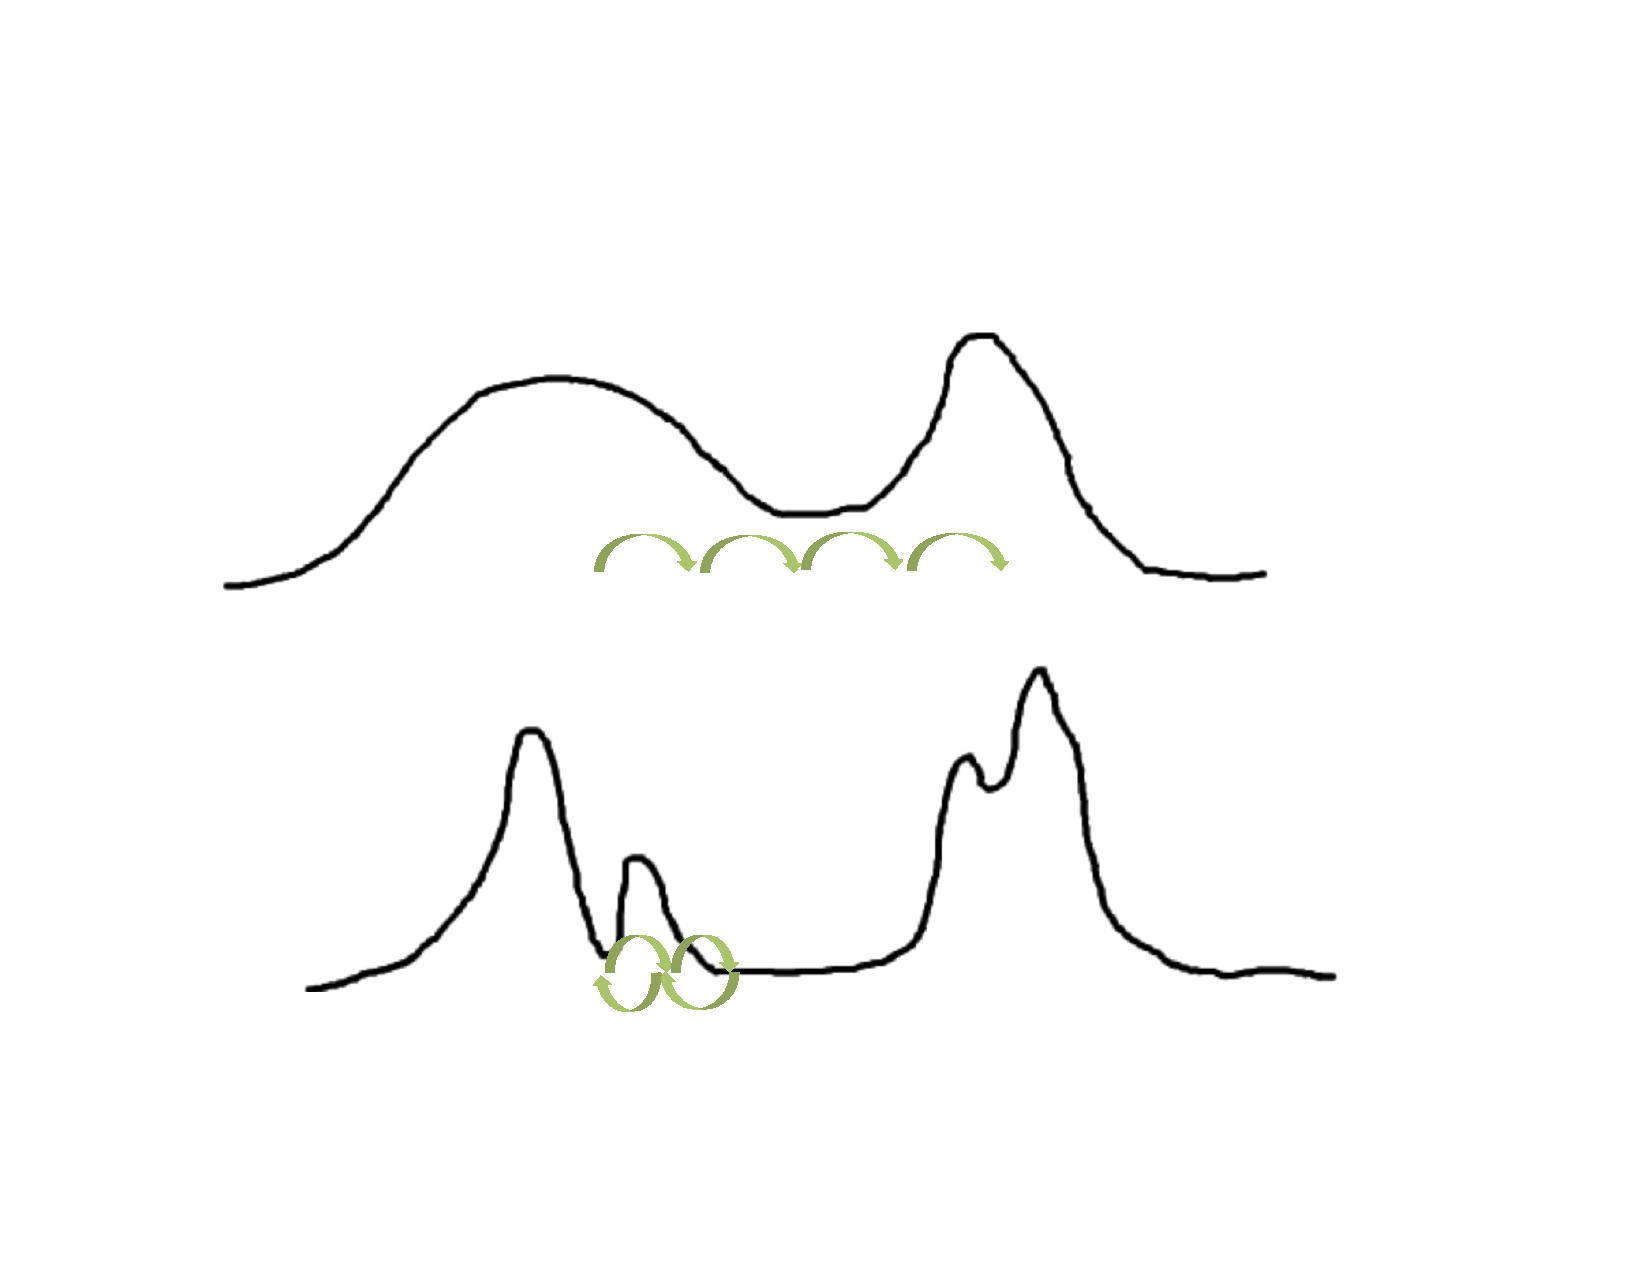
\includegraphics[width=0.75\linewidth]{article3/images/mixing-problem.pdf}}
\caption{\small Top: early during training, MCMC mixes easily between modes because the estimated
distribution has high entropy and puts enough mass everywhere for small-steps
movements (MCMC) to go from mode to mode. Bottom: later on, training relying
on good mixing can stall because estimated modes are separated by vast
low-density deserts.} \label{fig:mixing-issue}
\end{figure}


Another point worth discussing (and which should be considered in future
work) in {\bf H2} is the notion of {\em degree} of disentangling.  Although
it is somewhat clear what a completely disentangled representation would
look like, deep learning algorithms are unlikely to do a perfect job of
disentangling, and current algorithms do it in stages, with more abstract
features being extracted at higher levels. 
%In this paper, we consider cases
%where we know true underlying factors we seek to measure the strength of
%the statistical dependency (e.g., through mutual information) between
%latent variables of the representation and some of these known
%factors. 
Better disentangling would mean that {\em some} of the learned features
have a higher mutual information with {\em some} of the known factors. One would
expect at the same time that the features that are highly predictive of one
factor be less so of other factors, i.e., that they specialize to one or a
few of the factors, becoming {\em invariant} to others. Please note here
the difference between the objective of learning disentangled
representations and the objective of learning invariant features (i.e.,
invariant to some specific factors of variation which are considered to be
like nuisance parameters). In the latter case, one has to know ahead of
time what the nuisance factors are (what is noise and what is signal?).
In the former, it is not needed: we only seek to separate out the factors
from each other. Some features should be sensitive to one factor and
invariant to the others. 

Let us now consider additional hypotheses that specialize {\bf H2}.
\begin{center}
\framebox{
\begin{minipage}{0.8\linewidth}
{\bf Hypothesis H3: Disentangling Unfolds and Expands.} Part of the explanation of {\bf H2} is that
more disentangled representations tend to {\bf (a)} 
unfold the manifolds near which raw data concentrates, as well as
{\bf (b)} expand the relative volume occupied by high-probability points near
these manifolds.
\end{minipage}
}\\
\end{center} {\bf H3(a)} says is that disentangling has the effect that
the projection of high-density manifolds in the high-level representation space have a smoother
density and are easier to model than the corresponding high-density manifolds in raw
input space. Let us again use an object recognition analogy. If we have
perfectly disentangled object identity, pose and illumination, the
high-density manifold associated with the
distribution of features in high-level representation-space is flat: we can
interpolate between some training examples (i.e. likely configurations) and
yet stay in a high-probability region. For example, we can imagine that
interpolating between two images of the same object at different poses
(lighting, position, etc.) in a high-level representation-space would
yield images of the object at intermediate poses (i.e., corresponding to
likely natural images), whereas interpolating
in pixel space would give a superposition of the two original
images (i.e., unlike any natural image). If interpolating between high-probability
examples (i.e. within their convex set) gives high-probability examples, then
it means that the distribution is more uniform (fills the space) within
that convex set, which is what {\bf H3(b)} is saying. In addition, a good high-level
representation does not need to allocate as much real estate (sets of
values) for unlikely configurations. This is already what most unsupervised
learning algorithms tend to do. For example, dimensionality reduction
methods such as the PCA tend to define representations where most
configurations are likely (but these only occupy a subspace of the possible
raw-space configurations).  Also, in clustering algorithms such as k-means,
the training criterion is best minimized when clusters are approximately
equally-weighted, i.e., the average posterior distribution over cluster
identity is approximately uniform. Something similar is observed in the
brain where different areas of somatosensory cortex correspond to different
body parts, and the size of these areas adaptively depends~\citep{Flor-2003} 
on usage of these (i.e.,
more frequent events are represented more finely and less frequent ones are
represented more coarsely).  Again, keep in mind that the actual
representations learned by deep learning algorithms are not perfect, but
what we will be looking for here is whether deeper representations
correspond to more unfolded manifolds and to more locally uniform
distributions, with high-probability points occupying an overall greater
volume (compared to the available volume).

\vspace*{-1.5mm}
\section{Representation-Learning Algorithms}
\vspace*{-1mm}

The learning algorithms used in this paper to explore the preceding hypotheses are
the Deep Belief Network or DBN~\citep{Hinton06}, trained by stacking
Restricted Boltzmann Machines or RBMs, and the Contractive Auto-Encoder or
CAE~\citep{Rifai+al-2011}, for which a sampling algorithm was
recently proposed~\citep{Rifai-icml2012}.
In the experiments, the distribution under consideration is the asymptotic distribution
associated with the stochastic process used to generate samples. In the
case of DBNs it clearly corresponds to the analytically defined
distribution associated with the formula for the DBN probability.  The
Markov transition operator for DBNs is the one associated with Gibbs
sampling (in the top RBM)~\citep{Hinton06}. The Markov transition operator for stacked CAEs
has been spelled out in~\citet{Rifai-icml2012} and linked to
Langevin MCMC in~\citet{Alain+al-arxiv-2012}. 

Each layer of the DBN is trained as an RBM, and a 1-layer DBN is just an RBM. An RBM
defines a joint distribution between a hidden layer $h$ and a visible layer $v$. 
Gibbs sampling at the top level of the DBN is used to obtain samples from the
model: the sampled top-level representations are stochastically projected
down to lower levels through the conditional distributions $P(v|h)$
defined in each RBM. To avoid unnecessary additional noise, and like
previous authors have done, at the last stage of this process (i.e.
to obtain the raw-input level samples), only the mean-field values
of the visible units are used, i.e., $E[v|h]$. In the experiments on face
data (where grey levels matter a lot), a Gaussian RBM is used at the
lowest level. 

An auto-encoder~\citep{Lecun-these87,hinton1994amd} is parametrized
through an encoder function $f$ mapping input-space vector $x$ to
representation-space vector $h$, and a decoder function $g$ mapping
representation-space vector $h$ to input-space reconstruction $r$. The
experiments with the CAE are with $h=f(x)=\sigm(W x + b)$ and
$r=g(h)=\sigm(W^T h + c)$.  The CAE is a regularized auto-encoder with
tied weights (input to hidden weights are the transpose of hidden to
reconstruction weights). Let  $J=\frac{\partial f(x)}{\partial x}$ 
the Jacobian matrix of the encoder function. 
The CAE is trained to minimize a cross-entropy reconstruction
loss plus a contractive regularization penalty
$\alpha ||J||^2_F$ (the sum of the
squared elements of the Jacobian matrix). Like RBMs, CAE layers can be stacked to
form deeper models, and one can either view them as deep auto-encoders (by
composing the encoders together and the decoders together) or like in a
DBN, as a top-level generative model (from which one can sample) coupled with encoding
and decoding functions into and from the top level (by composing the lower-level
encoders and decoders).  A sampling algorithm was recently proposed for
CAEs~\citep{Rifai-icml2012},  alternating between projecting
through the auto-encoder (i.e. performing a reconstruction) and adding
Gaussian noise $J J^T \epsilon$ in the directions of variation captured by the auto-encoder.
%Some of the experiments reported
%here also make use of a variant of the CAE called the Manifold Tangent
%Classifier~\citep{Dauphin-et-al-NIPS2011} and that has achieved the
%best reported results on the MNIST dataset without using any explicit prior
%knowledge (no input deformations or convolutions).

\vspace*{-1.5mm}
\section{Experiments}
\vspace*{-1mm}

The experiments have been performed on the MNIST digits
dataset~\citep{LeCun98} and the Toronto Face
Database~\citep{Susskind2010}, TFD. The former has been heavily used to evaluate
many deep learning algorithms, while the latter is interesting because of
the manifold structure it displays, and for which the main control factors (such as
emotion and person identity) are known.

We have varied the number of hidden units at each layer independently for
shallow and deep networks, and the models that gave best validation
performance for each depth are shown. The qualitative aspects of the
results were insensitive to layer size.  The results reported are for DBNs with
768-1024-1024 layer sizes (28$\times$28 input) on MNIST, and 2304-512-1024 on TFD
(48$\times$48 input). The CAEs have sizes 768-1000-1000 and 2304-1000-1000
on MNIST and TFD respectively.

%%%%%%%%%%%%%%%%%%%%%%%%%%%%%%%%%%%%%%%%%%%%%%%%5

\iffalse
\section{TODO experiments}
Proximité entr les points aide le Mixing
- Yann: Histogramme de distance selon que c'est la même classe ou des
classes differentes. A partir des couples en utilisant AIS pour
calculer p(v_1|v_0)
- Salah: Mahalanobis sur les representations cachés a partir de couples.

Espace caché plus uniforme.
- Guillaume: Histogramme des p(v|h_i). Les configurations des h encodes
pour de plus grandes parties de l'espace.
- Greg: Mesurer l'erreur de reconstruction pour des configurations
aléatoire de h.

Disentangling.
- Yann: Mesure de mutual information, montrer que l'information se
concentre dans une plus petite partie du code.

Brainstorm:
1. Use the exact transition distance p(v_1|v_0) to calculate
distances. Maybe on a toy problem.
2. Comment réconcilier le fait qu'on mix mieux avec nos meilleur resultat
de classification?
	- Meilleur disentangling. Utilisation d'un bit reverse video
	- Guillaume: Certaines unités servent à la reconnaissance, certaines
	unités sont utiles pour le mixing.
	- la distribution du mutual information avec la classe
	est plus pointue sur les modèles profonds. Cela assume qu'il y a peu de
	facteur de variation utile pour la classification et qu'on les a bien
	isolé avec notre modèle.
	- 
3. Mesurer que les espaces sont plus uniformes quand on va dans les couches
profondes
	1.

\fi

\vspace*{-1mm}
\subsection{Sampling at Different Depths}
\vspace*{-1mm}
\subsubsection{Better Samples at Higher Levels}
\vspace*{-1mm}

To test {\bf H1}, we first plot sequences of samples at various depths. One can
verify in Fig.~\ref{fig:seq} that samples obtained at deeper layers are
visually more likely and mix faster between modes.

In addition, we measure the quality of the obtained samples, using a
procedure for the comparison of sample generators described in
\citet{Breuleux+Bengio-2011}.  Note that the mixing properties
measured here are a consequence of the underlying models
as well as of the chosen sampling procedures. For this reason, we have chosen
to monitor the {\em quality of the samples} with respect to the original
data generating distribution that was used to train the model.
The procedure of \citet{Breuleux+Bengio-2011} measures the log-likelihood of a test set
under the density computed from a Parzen window density estimator built on
generated samples ($10,000$ samples here). Log-likelihoods for different models are presented
in Table~\ref{tab:res-knn-svm} (rightmost columns).  Those results also suggest that the
quality of the samples is higher if the Markov chain process used for sampling
takes place in the upper layers.

This observation agrees with {\bf H3(b)} that moving in higher-level representation
spaces where the manifold has been expanded provides higher quality samples than
moving in the raw input space where it may be hard to stay in high density
regions.

\if0
\begin{table*}[ht]
  \begin{center}
\begin{tabular}{c|c|c|}
& MNIST & TFD \\ \hline
CAE-1 & $ 67.69\pm2.87$ & $591.90\pm12.27$\\
CAE-2 & $121.17\pm1.59$ & $2110.09\pm49.15$ \\\hline
DBN-1 & $-243.91\pm54.11$ & $604\pm14.67$ \\
DBN-2 & $137.89\pm2.11$ & $1908.80\pm65.94$ \\ \hline
\end{tabular}

\caption{Log-likelihoods from Parzen-Windows density estimators based on
$10,000$ samples generated by each model. This quantitatively confirms
that the samples generated from deeper levels are of higher quality, in
the sense of better covering the zones where test examples are found. } 
\label{tab:ll}

\end{center}

\end{table*}
\fi

\iffalse

\begin{figure*}
\begin{center}
\subfigure[DBN Layer 1]
{\hspace*{-2mm}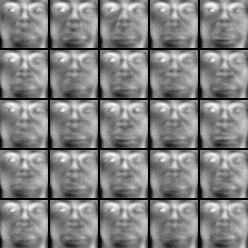
\includegraphics[width=0.24\textwidth]{article3/images/samplesTFDlayer1.png}}
\subfigure[DBN Layer 2]
{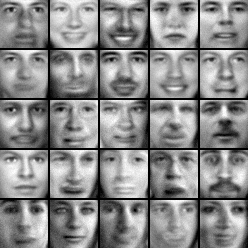
\includegraphics[width=0.24\textwidth]{article3/images/samplesTFDlayer2.png}}
\subfigure[CAE Layer 1]
{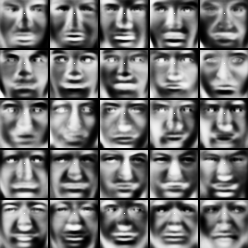
\includegraphics[width=0.24\textwidth]{article3/images/batch3cae1tfddata_image_noncen.png}}
\subfigure[CAE Layer 2]
{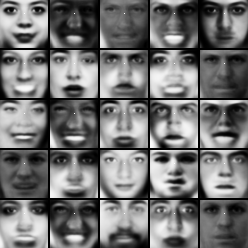
\includegraphics[width=0.24\textwidth]{article3/images/cae2tfd_folder15data_image_noncen.png}} \\
\subfigure[DBN Layer 1]
{\hspace*{-2mm}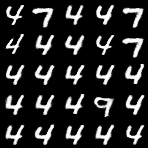
\includegraphics[width=0.24\textwidth]{article3/images/newrbm1mnistdata_image_noncen.png}}
\subfigure[DBN Layer 2]
{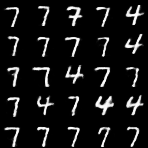
\includegraphics[width=0.24\textwidth]{article3/images/newrbm2mnistdata_image_noncen.png}}
\subfigure[CAE Layer 1]
{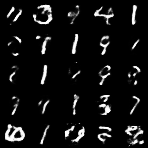
\includegraphics[width=0.24\textwidth]{article3/images/cae2mnistdata.png}}
\subfigure[CAE Layer 2]
{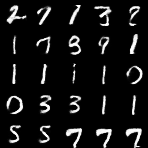
\includegraphics[width=0.24\textwidth]{article3/images/cae2mnistdata_image_noncen.png}}
\end{center}

\caption{Samples from DBNs and CAEs with 1 or 2 layers on TFD (top) and MNIST (bottom).
We see that samples from the second level are generally of better quality than samples
of the first level.}

\label{fig:samples}
\end{figure*}
\fi

%\subsubsection{Visualizing Trajectories of Samples in Representation-Space}
%
%
%Instead of viewing isolated samples, let us consider the temporal aspect of the
%Markov chain sampling process to get some insight about the structure of
%the learned representation-space. 
%{\bf H1} assumes that mixing is easier if you
%sample from the upper layers rather than using the lower layers. In
%Fig.~\ref{fig:seq}, the sequences of $25$ samples presented suggest that mixing
%is indeed easier on deeper layers and generates more likely samples.
%The last
%statement is also going in the same direction as the {\bf H3(b)} (avoid repetition
%with last section).
%
%\fix{More quantitative measures are explored in Sec.~\ref{sec:mix-time} such as jumping time
%among classes.}

\begin{figure*}
\vspace*{-3mm}
\begin{center}
%\subfigure[CAE Layer 1 on TFD]
%{
    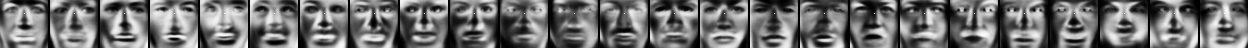
\includegraphics[width=0.95\textwidth]{article3/images/cae1tfd_seq4_data_image_noncen.png}
%    }
%\subfigure[CAE Layer 2 on TFD]
%{
    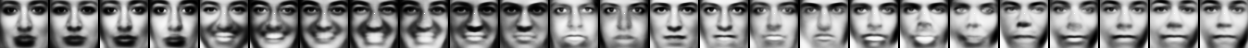
\includegraphics[width=0.95\textwidth]{article3/images/cae2tfd_seq6_data_image_noncen.png}
    
\includegraphics[width=0.95\textwidth]{article3/images/rbm1mnist_seq3_data_image_noncen.png}
    
\includegraphics[width=0.95\textwidth]{article3/images/rbm2mnist_seq17_data_image_noncen.png}
%    }
\end{center}
\vspace*{-3mm}
\caption{Sequences of $25$ samples generated with a CAE
on TFD (rows 1 and 2, respectively for 1 or 2 hidden layers) 
and with an RBM on MNIST (rows 3 and 4, respectively for 1 or
2 hidden layers). 
{\small On TFD, the second layer clearly allows to get
quickly from woman samples (left) to man samples (right) passing by various facial
expressions whereas the single hidden layer model shows poor samples.
Bottom rows: On MNIST, the single-layer model gets stuck
near the same mode while the second layer allows to mix among classes.}  }

\label{fig:seq}
\vspace*{-3mm}
\end{figure*}


\vspace*{-1mm}
\subsubsection{Visualizing Representation-Space by Interpolating Between Neighbors}
\vspace*{-1mm}

According to {\bf H3(a)}, deeper layers tend to locally unfold the manifold
near high-densities regions of the input space, while according to {\bf H3(b)}
there should be more relative volume taken by plausible configurations in representation-space.
Both of these would imply that convex combinations of neighboring examples in representation-space
correspond to more likely input configurations. Indeed, interpolating between
points on a flat manifold should stay on the manifold. Furthermore, when interpolating
between examples of different classes (i.e., different modes), {\bf H3(b)} would
suggest that most of the points in between (on the linear interpolation line)
should correspond to plausible samples, which would not be the case in input space.
In Fig.~\ref{fig:interpol}, we interpolate linearly between neighbors in
representation space and visualize in the input space the interpolated points obtained at
various depths. One can see that interpolating at deeper levels gives visually
more plausible samples.

\begin{figure}
\centering
\begin{subfigure}{1.\textwidth}
\caption{Interpolating between an example and its $200$-th nearest neighbor (see caption below).}
    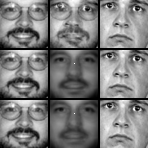
\includegraphics[width=0.24\textwidth]{article3/images/100interpolationtfdfold1_cae2_samples812data_image_noncen.png}
    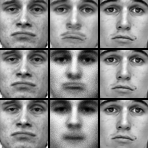
\includegraphics[width=0.24\textwidth]{article3/images/100interpolationtfdfold1_rbm2_samples1data_image_noncen.png}
    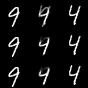
\includegraphics[width=0.24\textwidth]{article3/images/200interpolationmnist28_cae2_samples1data_image_noncen.png}
    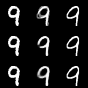
\includegraphics[width=0.24\textwidth]{article3/images/200interpolationmnist28_rbm2_samples51data_image_noncen.png}
\end{subfigure}
\begin{subfigure}{1.\textwidth}
\caption{Interpolating between an example and its nearest neighbor.}
    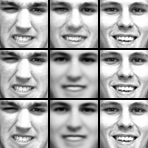
\includegraphics[width=0.24\textwidth]{article3/images/1interpolationtfdfold1_cae2_samples6data_image_noncen.png}
    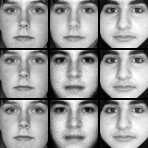
\includegraphics[width=0.24\textwidth]{article3/images/1interpolationtfdfold1_rbm2_samples2data_image_noncen.png}
    
\includegraphics[width=0.24\textwidth]{article3/images/1interpolationmnist28_cae2_samples28data_image_noncen.png}
    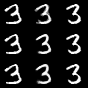
\includegraphics[width=0.24\textwidth]{article3/images/1interpolationmnist28_rbm2_samples16data_image_noncen.png}
\end{subfigure}

\begin{subfigure}{1.\textwidth}
\caption{Sequences of points interpolated at different depths}
    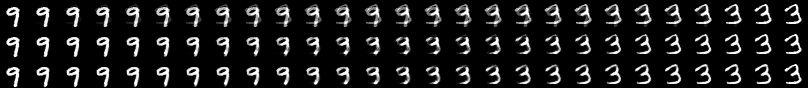
\includegraphics[width=0.96\textwidth]{article3/images/sequenceinterpolation46_data_image_noncen.png}
    \label{fig:seqinterpol}
\end{subfigure}

\caption{ Linear interpolation between a data sample and the 200-th (a)
and 1st (b) nearest neighbor, using representations 
at various depths (top row=input space, middle row=1st layer,
bottom row=2nd layer).  In each $3\times3$ block the left and right columns are
test examples while the middle column is the image obtained by interpolation, based on
different levels of representation.
Interpolating at higher levels clearly gives more plausible samples. Especially in
the raw input space (e.g., (a), 2nd block), one can see two mouths overlapping while only one mouth appears
for the interpolated point at the 2nd layer. Interpolating with the 1-nearest neighbor
does not show any difference between the levels because the nearest neighbors are close enough
for a linear interpolation to be meaningful, while interpolaing with the 200-th nearest
neighbors shows the failure of interpolation in raw input space but successful
interpolation in deeper levels. In (c), we interpolate between samples
of {\em different classes}, at different depths (top=raw input, middle=1st layer, bottom=2nd layer).
Note how in lower levels one has to go through unplausible patterns, whereas in the deeper
layers one almost jumps from a high-density region of one class to another (of the other class).}
\label{fig:interpol}
\end{figure}




\vspace*{-1mm}
\subsection{Measuring Mixing Between Modes by Counting Number of Classes Visited}
\label{sec:mix-time}
\vspace*{-1mm}

We evaluate here the ability of mixing among various classes. We consider sequences
of length 10, 20 or 100 and compute histograms of number of different classes visited
in a sequence, for the two different depths and learners, on TFD. Since classes
typically are in different modes (manifolds), counting how many different classes
are visited in an MCMC run tells us how quickly the chain mixes between modes.
We have chosen this particular method to monitor mixing modes because it focuses more
directly on visits to modes, instead of the traditional autocorrelation of the
samples (which measures how fast the samples change).
Fig.~\ref{fig:entropy}(c,f) show that the deeper architectures visit more classes
and the CAE mixes faster than the DBN. 

\vspace*{-1mm}
\subsection{Occupying More Volume Around Data Points}
\vspace*{-1mm}

In these experiments (Fig.~\ref{fig:entropy} (a,b,d,e)) we estimate the quality of samples whose representation is in
the neighborhood of training examples, at different levels of representation.
In the first setting (Fig.~\ref{fig:entropy} (a,b)), the samples are interpolated at the midpoint
between an example and its $k$-th nearest neighbor, with $k$ on the x-axis. 
In the second case (Fig.~\ref{fig:entropy} (d,e)),
isotropic noise is added around an example, with noise standard deviation on the x-axis. 
In both cases, 500 samples are generated
for each data point plotted on the figures, with the y-axis being the log-likelihood
introduced earlier, i.e., estimating the quality of the samples.
We find that on higher-level representations of both the CAE and DBN, a much
larger proportion of the local volume is occupied by likely configurations,
i.e., closer to the input-space manifold near which the actual data-generating
distribution concentrates. Whereas the first experiment shows that this is true
in the convex set between neighbors at different distances (i.e., in the directions
of the manifold), the second shows that this is also true in random directions locally
(but of course likelihoods are also worse there). The first result therefore
agrees with {\bf H3(a)} (unfolding) and {\bf H3(b)} (volume expansion), while
the second result mostly confirms {\bf H3(b)}.
\begin{figure}
\centering

\begin{subfigure}{.45\textwidth}
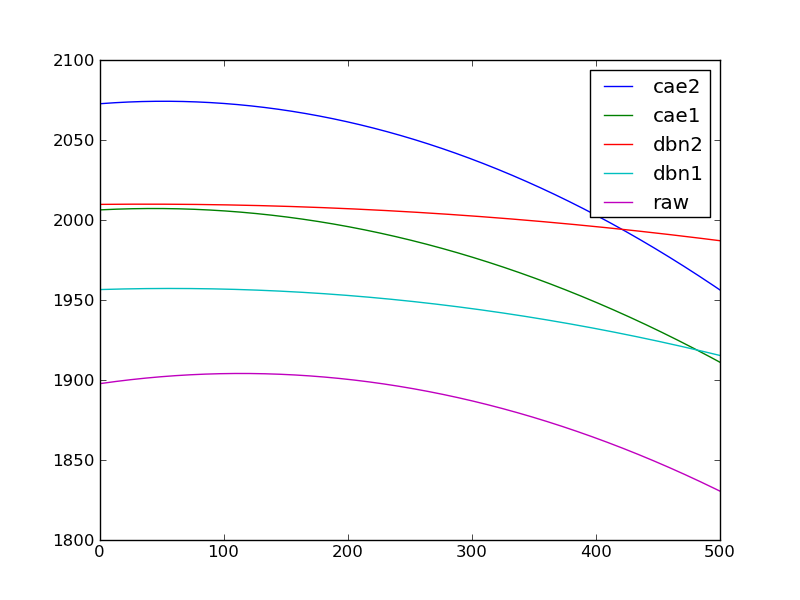
\includegraphics[width=1.\textwidth]{article3/images/tfdfold1_degree2_new2.png}
\caption{TFD}
\end{subfigure}
\begin{subfigure}{.45\textwidth}
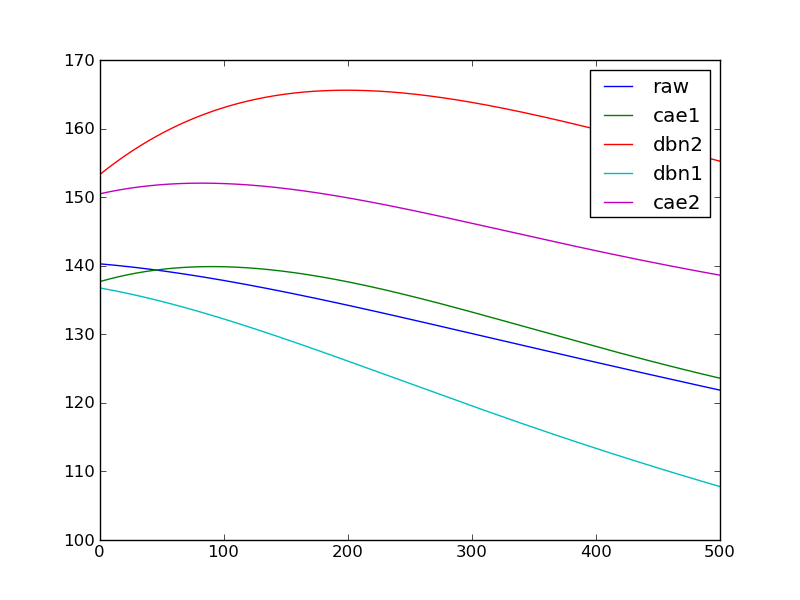
\includegraphics[width=1.\textwidth]{article3/images/mnist28_degree4dbnlegend.png}
\caption{MNIST}
\end{subfigure}

\begin{subfigure}{.45\textwidth}
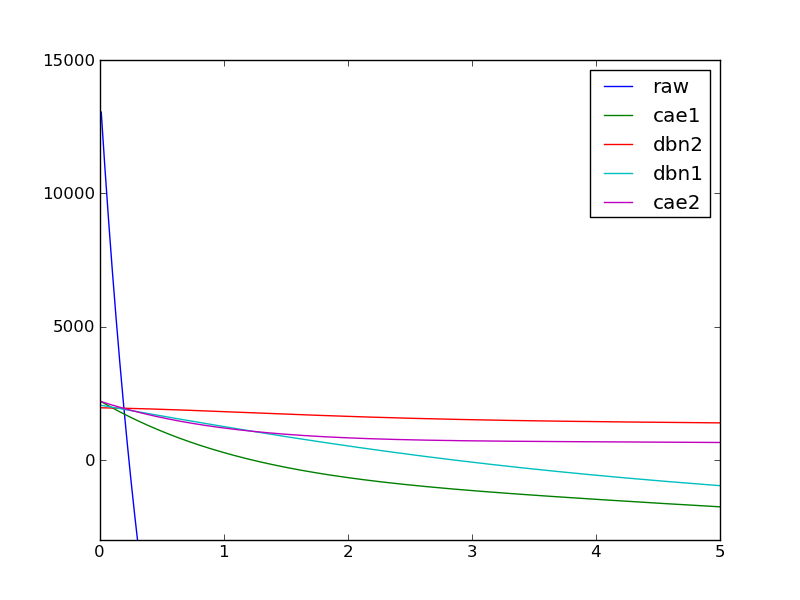
\includegraphics[width=1.\textwidth]{article3/images/tfdfold1_degree6.png}
\caption{TFD}
\end{subfigure}
\begin{subfigure}{.45\textwidth}
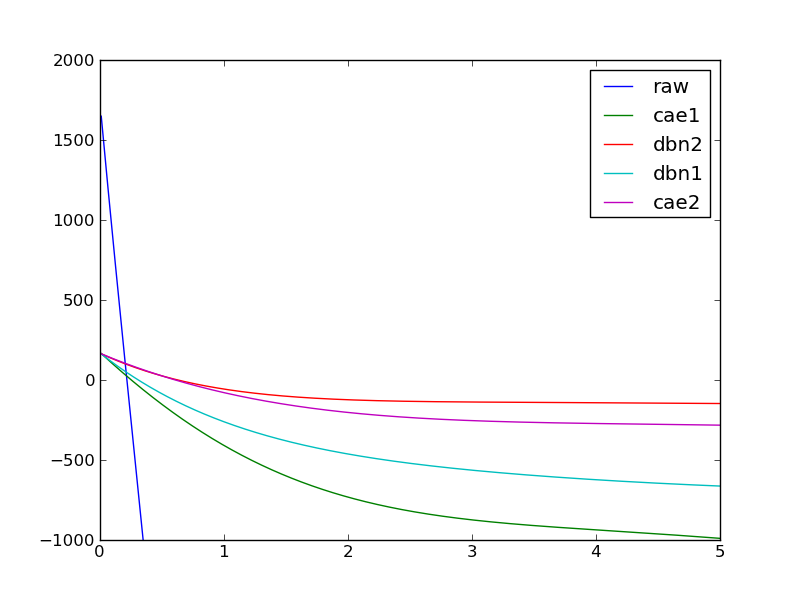
\includegraphics[width=1.\textwidth]{article3/images/convexball_mnist28_degree6.png}
\caption{MNIST}
\end{subfigure}

\begin{subfigure}{.45\textwidth}
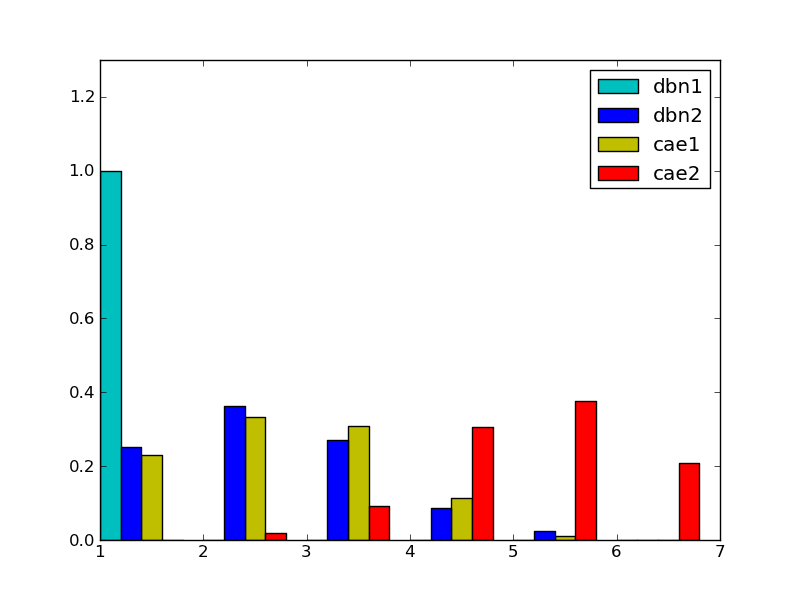
\includegraphics[width=1.\textwidth]{article3/images/tfd_sub0.png}
\caption{Mixing - 10 samples}
\end{subfigure}
\begin{subfigure}{.45\textwidth}
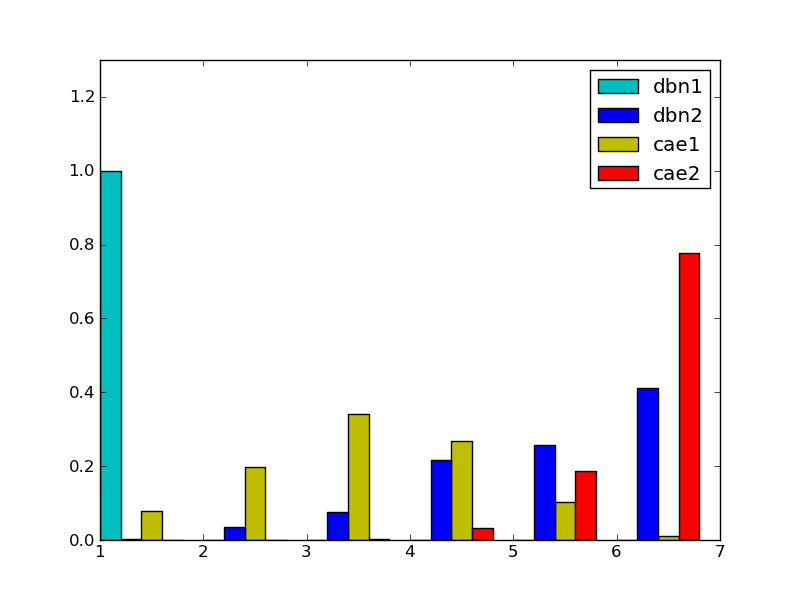
\includegraphics[width=1.\textwidth]{article3/images/tfd_sub1.png}
\caption{Mixing - 20/100 samples}
\end{subfigure}

\caption{ (a) (b) Local Convex Hull - Log-density computed w.r.t. linearly
interpolated samples between an example and its k-NNs, for k (x-axis)
between 1 and 500. The manifold thus seem generally more unfolded (flatter)
in deeper levels, especially against raw input space,
as interpolating between far points yields higher density
under deeper representations.
(c) (d) Local Convex Ball -
Log-density of samples generated by adding Gaussian noise to representation
at different levels ($\sigma\in[0.01,5]$, the x-axis): More volume is
occupied by good samples on
deeper layers. (e) (f) Mode Mixing Histograms - distribution (y-axis)
of number of classes visited (x-axis) for different
models. (e) with 10 samples. (f) with 20 samples for CAE, 100 samples with DBN. Deeper
models mix much better.}
\label{fig:entropy}
\end{figure}


%\resizebox{0.8\linewidth}{!}{
%\scalebox{0.8}{
\begin{table*}[!htbp]
\begin{small}
 \begin{center}
\begin{tabular}{c|c|c||c|c||c|c|}
& \multicolumn{4}{|c||}{\bf Classification} & \multicolumn{2}{|c|}{\bf Log-likelihood}  \\ \hline
& \multicolumn{2}{|c||}{\bf MNIST} & \multicolumn{2}{c||}{\bf TFD} & \multicolumn{1}{|c|}{\bf MNIST} & \multicolumn{1}{c|}{\bf $\,\,\,$TFD $\,\,\,\,$}\\
& SVM &  MLP+ & SVM  & MLP+ & & \\ \hline
raw   & 8.34\%  & -      & $33.48$ {\scriptsize $\pm 2.14$ }\% & - & - & - \\ \hline
CAE-1 & 1.97\%  & 1.14\% & $25.44$ {\scriptsize $ \pm2.45$}\% & $24.12$ {\scriptsize $\pm1.87$} \% & $ 67.69$ {\scriptsize $\pm2.87$} & $591.90$ {\scriptsize $\pm12.27$}\\
CAE-2 & 1.73\%  & 0.81\% & $24.76$ {\scriptsize $\pm2.46$}\% & $23.73$ {\scriptsize $\pm1.62$}\% & $121.17$ {\scriptsize $\pm1.59$} & $2110.09$ {\scriptsize $\pm49.15$}\\ \hline
DBN-1 & 1.62\%  & 1.21\% & $26.85$ {\scriptsize $\pm1.62$}\% & $28.14${\scriptsize $\pm1.40 $}  & $-243.91$ {\scriptsize $\pm54.11$} &  $604$ {\scriptsize $\pm14.67$} \\
DBN-2 & 1.33\%  & 0.99\% & $26.54$ {\scriptsize $\pm1.91$}\% & $27.79$ {\scriptsize $\pm2.34$}& $137.89$ {\scriptsize $\pm2.11$} & $1908.80$ {\scriptsize $\pm65.94$}\\\hline
\end{tabular}

\caption{Left: Classification rates of various classifiers (SVM, MLP+)
  using representations at various depth (with CAE or DBN)
  learned on the MNIST and TFD datasets.  The DBN 0.99\% error on
  MNIST has been obtained with a 3-layer DBN and the 0.81\% error
  with the Manifold tangent
  Classifier~\citep{Dauphin-et-al-NIPS2011} that is based on a
  CAE-2 and discriminant fine-tuning. MLP+ uses discriminant
  fine-tuning. Right: Log-likelihoods from Parzen-Windows density
  estimators based on $10,000$ samples generated by each model. This
  quantitatively confirms that the samples generated from deeper
  levels are of higher quality, in the sense of better covering the
  zones where test examples are found.}
\label{tab:res-knn-svm}

\end{center}
\end{small}
\end{table*}

\vspace*{-1mm}
\subsection{Discriminative Ability vs Volume Expansion}
\vspace*{-1mm}

Hypothesis {\bf H3} could arguably correspond to worse discriminative 
power\footnote{\scriptsize as pointed out by Aaron Courville, personal communication}:
if on the higher-level representations the different classes are ``closer''
to each other (making it easier to mix between them), would it not mean that they
are more confusable? We first confirm with the tested models (as a sanity check)
that the deeper level features are conducive to better classification performance,
in spite of their better generative abilities and better mixing between modes.

\if0
\begin{table*}[ht]
  \begin{center}
\begin{tabular}{c|c|c|c||c|c|c|}
& \multicolumn{3}{|c||}{\bf MNIST} & \multicolumn{3}{c|}{\bf TFD}\\
& SVM & k-NN & NN & SVM & k-NN & NN \\ \hline
raw   & 8.34\%         & 3.42\% & -      & $33.48\pm 2.14$\% & $45.37\pm2.27$\% & -\\ \hline
CAE-1 & 1.89\%+1.97\%  & 2.91\% & 1.14\% & $28.44\pm2.70$\%+$25.44\pm2.45$\% & ???+$45.83\pm1.97$\% & $24.12\pm1.87$ \%\\
CAE-2 & 1.88\%+1.73\%  & 2.91\% & ???\%  & $28.58\pm2.16$\%+$24.76\pm2.46$\% & ???+$46.71\pm2.22$\% & $23.73\pm1.62$\% \\ \hline
DBN-1 & 1.40\%+1.62\%  & 2.49\% & 1.21\% & ???             +$26.85\pm1.62$\% & ???+$37.55\pm1.46$\%  & ???\\
DBN-2 & 1.23\%+1.33\%  & 2.61\% & ???    & ???             +$26.54\pm1.91$\% & ???+$37.39\pm1.49$\%  & ??? \\\hline
\end{tabular}

\caption{ {\bf Left: Classification rates using various classifiers on
representations learned on the MNIST and TFD datasets} left is on the
top of the repressentation and right on the concatentation of raw
input and upper layers (we'll have to choose one). Right:
Log-likelihoods from Parzen-Windows density estimators based on
$10,000$ samples generated by each model. This quantitatively confirms
that the samples generated from deeper levels are of higher quality,
in the sense of better covering the zones where test examples are
found. } \label{tab:res-knn-svm}

\end{center}

\end{table*}
\fi

We train a linear SVM on the concatenation of the raw input with the upper
layers representations (which worked better than using only the top layer,
a setup already used successfully when there is no supervised fine-tuning~\citep{HonglakLNIPS2009-small}).  
Results presented in Table~\ref{tab:res-knn-svm} show
that the representation is more linearly separable if one increases the depth of
the architecture and the information added by each layer is helpful for
classification. Also, fine-tuning a MLP initialized with those weights is still
the best way to reach state-of-the-art performances.  

To explain the good discriminant abilities of the deeper layers (either
when concatenated with lower layers or when fine-tuned discriminatively)
in spite of the better mixing observed, we conjecture the help of a
better disentangling of the underlying factors of variation, and in 
particular of the class factors. This would mean that the manifolds associated 
with different classes are more unfolded (as assumed by {\bf H3(a)}) and possibly
that different hidden units specialize more to specific classes than they
would on lower layers. Hence the unfolding ({\bf H3(a)})
and disentangling ({\bf H1}) hypotheses reconcile better discriminative ability
with expanded volume of good samples ({\bf H3(b)}).

%Also, exemples from the same class tend to be more clusterized in the
%representation-space compared to the input space since the error of the k-NN
%classifier decrease with the depth.

\iffalse
\subsubsection{Measuring Disentangling}

\begin{figure*}
\begin{center}
\subfigure[TFD]
{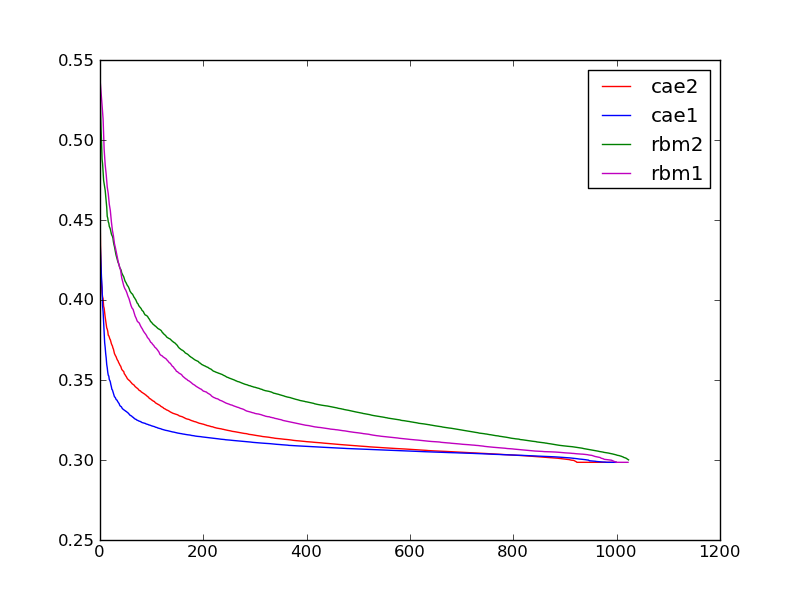
\includegraphics[width=0.49\textwidth]{images/tfd_MI.png}}
\subfigure[MNIST]
{\includegraphics[width=0.49\textwidth]{images/mtc_MI.png}}
\end{center}

\caption{ {\bf Mutual Information between Classes and hidden units at various
depth}}
\label{fig:MI}
\end{figure*}

In Fig.~\ref{fig:MI}, we measured the mutual information between each hidden
unit and classes at different depths.  The curve is sharper for lower layers
suggesting that hidden units at deeper layers encode more discriminative
factors of variation than lower layer's units. 
\fi



\vspace*{-2mm}
\section{Conclusion}
\vspace*{-2mm}

The following hypotheses were tested: (1) deeper representations can yield better samples
and better mixing between modes; (2) this is due to better disentangling; (3) this is associated with
unfolding of the manifold where data concentrate along with expansion of the volume
good samples take in representation-space. The experimental results were in agreement
with these hypotheses. They showed better samples and better mixing on higher levels,
better samples obtained when interpolating between examples at higher levels, and
better samples obtained when adding isotropic noise at higher levels. We also considered
the potential conflict between the third hypothesis and better discrimination
(confirmed on the models tested) and explained it away as a consequence of the second
hypothesis.

This could be immediate good news for applications requiring to generate MCMC samples:
by transporting the problem to deeper representations, better and faster results could
be obtained. Future work should also investigate the link between better mixing
and the process of training deep learners themselves, when they depend on an MCMC to estimate the log-likelihood
gradient.  One interesting direction is to investigate the link between tempering and
the better mixing chains obtained from deeper layers.\\
%One option is that higher levels of the hierarchy could be used in a way
%similar to higher-temperature chains in parallel tempering MCMC, i.e., by providing
%good starting points for lower level chains and doing the hard work of jumping
%between the modes associated with the lower levels.

\section{Acknowledgements}

The authors thank A. Courville and P. Vincent for fruitful discussions, as
well as NSERC, Canada Research Chairs, CIFAR, Compute Canada and by the French 
ANR Project ASAP ANR-09-EMER-001. Codes for the experiments have been implemented using the
Theano \citep{bergstra+al:2010-scipy} Machine Learning libraries.

%\vspace*{-3mm}
%{\small
%\bibliography{strings,strings-shorter,ml,myrefs,aigaion-shorter}
%\bibliography{strings,strings-shorter,ml,aigaion-shorter}
%\bibliographystyle{plain}
%\bibliographystyle{natbib}
%}


%\end{document}

\chapter{Pr\'{e}ambule au Quatri\`{e}me Article }

\section{D\'{e}tails de l'article}

\section{Contexte}

\section{Contributions}

\section{R\'{e}cents d\'{e}veloppements}


\chapter{Using Recurrent Neural Networks for Slot Filling in Spoken Language Understanding}
\label{chap:rnn}

\section{Introduction}

The term "spoken language understanding" (SLU) refers to the targeted
understanding of human speech directed at machines [1]. The goal of such
"targeted" understanding is to convert the recognition of user input, $S_i$, into
a task-specific semantic representation of the user's intention, $U_i$ at each
turn. The dialog manager then interprets $U_i$ and decides on the most
appropriate system action, $A_i$, exploiting semantic context, user specific
meta-information, such as geo-location and personal preferences, and other
contextual information.

The semantic parsing of input utterances in SLU typically consists of three
tasks: domain detection, intent determination, and slot filling. Originating
from call routing systems, the domain detection and intent determination tasks
are typically treated as semantic utterance classification problems [2,3,4,30].
Slot filling is typically treated as a sequence classification problem in which
contiguous sequences of words are assigned semantic class labels.
[5,7,31,32,33,34,40,55]. 

In this paper, following the success of deep learning methods for semantic
utterance classification such as domain detection [30] and intent determination
[13,39,50], we focus on applying deep learning methods for slot filling.
Standard approaches to solving the slot filling problem include generative
models, such as HMM/CFG composite models [31,5,53], hidden vector state (HVS)
model [33], and discriminative or conditional models such as conditional random
fields (CRFs) [6,7,32,34,40,51,54] and support vector machines (SVMs) [52].
Despite many years of research, the slot filling task in SLU is still a
challenging problem, and this has motivated the recent application of a number
of very successful continuous-space, neural net, and deep learning approaches,
e.g. [13,15,24,30,56]. 

In light of the recent success of these methods, especially the success of RNNs
in language modeling [22,23] and in some preliminary SLU experiments
[15,24,30,56], in this paper we carry out an in-depth investigation of RNNs for
the slot filling task of SLU. In this work, we implemented and compared several
important RNN architectures, including the Elman-type networks [16],
Jordan-type networks [17] and their variations. To make the results easy to
reproduce and rigorously comparable, we implemented these models using the
common Theano neural network toolkit [25] and evaluated them on the standard
ATIS (Airline Travel Information Systems) benchmark. We also compared our
results to a baseline using conditional random fields (CRF). Our results show
that on the ATIS task, both Elman-type networks and Jordan-type networks
outperform the CRF baseline substantially, and a bi-directional Jordan-type
network that takes into account both past and future dependencies among slots
works best.

In the next section, we formally define the semantic utterance
classification problem along with the slot filling task and present the
related work. In Section \ref{sec:deepreview}, we propose a brief review of deep learning
for slot filling. Section \ref{sec:rnnsf} more specifically describes our approach of
RNN architectures for slot filling. We describe sequence level
optimization and decoding methods in Section \ref{sec:slod}. Experimental results
are summarized and discussed in section \ref{sec:exp}.

\section{Slot Filling in Spoken Language Understanding}
\label{sec:sfslu}

A major task in spoken language understanding in goal-oriented human-machine
conversational understanding systems is to automatically extract semantic
concepts, or to fill in a set of arguments or "slots" embedded in a semantic
frame, in order to achieve a goal in a human-machine dialogue. 

An example sentence is provided here, with domain, intent, and slot/concept
annotations illustrated, along with typical domain-independent named entities.
This example follows the popular in/out/begin (IOB) representation, where {\it
Boston} and {\it New York} are the departure and arrival cities specified as
the slot values in the user's utterance, respectively.

TODO TABLE IOB REPRESENTATION

While the concept of using semantic frames (templates) is motivated by the case
frames of the artificial intelligence area, the slots are very specific to the
target domain and finding values of properties from automatically recognized
spoken utterances may suffer from automatic speech recognition errors and poor
modeling of natural language variability in expressing the same concept. For
these reasons, spoken language understanding researchers employed statistical
methods. These approaches include generative models such as hidden Markov
models, discriminative classification methods such as CRFs, knowledge-based
methods, and probabilistic context free grammars. A detailed survey of these
earlier approaches can be found in [7].

For the slot filling task, the input is the sentence consisting of a sequence
of words, $L$, and the output is a sequence of slot/concept IDs, $S$, one for each
word. In the statistical SLU systems, the task is often formalized as a pattern
recognition problem:  Given the word sequence $L$, the goal of SLU is to find the
semantic representation of the slot sequence $S$ that has the maximum {\it a
posteriori} probability $P(S | L)$. 

In the generative model framework, the Bayes rule is applied:

TODO EQUATION %S ̂= argmax_S P(S│L)=argmax_S P(L│S)P(S)

The objective function of a generative model is then to maximize the joint
probability $P(L | S)P(S) = P(L, S)$ given a training sample of $L$, and its semantic
annotation, $S$.

The first generative model, used by both the AT\&T CHRONUS system [31] and the
BBN Hidden Understanding Model (HUM) [35], assumes a deterministic one-to-one
correspondence between model states and the segments, i.e., there is only one
segment per state, and the order of the segments follows that of the states.  

As another extension, in the Hidden Vector State model the states in the
Markov chain representation encode all the structure information about the
tree using stacks, so the semantic tree structure (excluding words) can be
reconstructed from the hidden vector state sequence. The model imposes a hard
limit on the maximum depth of the stack, so the number of the states becomes
finite, and the prior model becomes the Markov chain in an HMM [33].

Recently, discriminative methods have become more popular. One of the most
successful approaches for slot filling is the conditional random field (CRF)
[6] and its variants. Given the input word sequence $L_1^N=l_1,\dots,l_N$, the
linear-chain CRF models the conditional probability of a concept/slot sequence
$S_1^N=s_1,\dots,s_N$ as follows:

TODO EQUATION NUM% P(S_1^N│L_1^N )=1/Z ∏_(t=1)^N▒e^(H(s_(t-1),s_t,l_(t-d)^(t+d)))             
%where EQUATION NUM 2 H(s_(t-1),s_t,l_(t-d)^(t+d) )=∑_(m=1)^M▒〖λ_m h_m (s_(t-1),s_t,l_(t-d)^(t+d))〗

and $h_m (s_{t-1},s_t,l_{t-d}^{t+d})$ are features extracted from the current and
previous states $s_t$ and $s_{t-1}$, plus a window of words around the current word
$l_t$, with a window size of $2d+1$.

CRFs have first been used for slot filling by Raymond and Riccardi [33]. CRF
models have been shown to outperform conventional generative models. Other
discriminative methods such as the semantic tuple classifier based on SVMs [36]
has the same main idea of semantic classification trees as used by the Chanel
system [37], where local probability functions are used, i.e., each phrase is
separately considered to be a slot given features. More formally,

TODO EQNUM 3 % P(S_1^N│L_1^N )=∏_(t=1)^N▒〖P(s_t |s_1^(t-1),L_1^N)〗   (3)

These methods treat the classification algorithm as a black box implementation
of linear or log-linear approaches but require good feature engineering. As
discussed in [57,13], one promising direction with deep learning architectures
is integrating both feature design and classification into the learning
procedure.

\section{Deep Learning Review}
\label{sec:deepreview}

In comparison to the above described techniques, deep learning uses many layers
of neural networks [57]. It has made strong impacts on applications ranging
from automatic speech recognition [8] to image recognition [10]. 

A distinguishing feature of NLP applications of deep learning is that inputs
are symbols from a large vocabulary, which led the initial work on neural
language modeling [26] to suggest map words to a learned distributed
representation either in the input or output layers (or both), with those
embeddings learned jointly with the task. Following this principle, a variety
of neural net architectures and training approaches have been successfully
applied [11,13,20,22,23,39,49,58,59,60,61]. Particularly, RNNs [22,23,49] are
also widely used in NLP. One can represent an input symbol as a one-hot vector,
i.e., containing zeros except for one component equal to one, and this weight
vector is considered as a low-dimensional continuous valued vector
representation of the original input, called word embedding. Critically, in
this vector space, similar words that have occurred syntactically and
semantically tend to be placed by the learning procedure close to each other,
and relationships between words are preserved. Thus, adjusting the model
parameters to increase the objective function for a training example which
involves a particular word tends to improve performances for similar words in
similar context, thereby greatly improving generalization and addressing the
curse-of-dimensionality obstacle faced with traditional n-gram non-parametric
models [26].

One way of building a deep model for slot filling is to stack several neural
network layers on top of each other. This approach was taken in [27], which
used deep belief networks (DBNs), and showed superior results to a CRF baseline
on ATIS. The DBNs were built with a stack of Restricted Boltzmann Machines
(RBMs) [12]. The RBM layers were pre-trained to initialize the weights. Then
the well-known back-propagation algorithm was used to fine-tune the weights of
the deep network in a discriminative fashion. Once the individual local models
are trained, Viterbi decoding is carried out to find the best slot sequence
given the sequence of words. 

In contrast to using DBNs, we propose recurrent neural networks (RNNs). The
basic RNNs used in language modeling read an input word and predict the next
word. For SLU, these models are modified to take a word and possibly other
features as input, and to output a slot value for each word. We will describe
RNNs in detail in the following section. 

\section{Recurrent Neural Networks for Slot-Filling}
\label{sec:rnnsf}

We provide here a description of the RNN models used for the slot filling task. 

\subsection{Words Embeddings}

The main input to a RNN is a one-hot representation of the next input word. The
first-layer weight matrix defines a vector of weights for each word, whose
dimensionality is equal to the size of the hidden layer (Fig.~\ref{fig:rnn}) - typically a
few hundred. This provides a continuous-space representation for each word.
These neural word embeddings [26] may be trained a-priori on external data such
as the Wikipedia, with a variety of models ranging from shallow neural networks
[21] to convolutional neural networks [20] and RNNs [22]. Such word embeddings
actually present interesting properties [23] and tend to cluster [20] when
their semantics are similar.

\begin{figure}[t]
\begin{center}
\includegraphics[width=.8\linewidth]{article4/images/rnn.png}
\caption{\label{fig:rnn} Three different types of neural networks 
(a) Feed-forward NN; (b) Elman-RNN; (c) Jordan-RNN}
\vspace{-0.2in}
\end{center}
\vspace*{-1mm}
\end{figure}


While [15][24] suggest initializing the embedding vectors with unsupervised
learned features and then fine-tune it on the task of interest, we found that
directly learning the embedding vectors initialized from random values led to
the same performance on the ATIS dataset, when using the SENNA
\footnote{http://ml.nec-labs.com/senna/} word embeddings. While this behavior
seems very specific to ATIS, we considered extensive experiments about
different unsupervised initialization techniques out of the scope of this
paper. Word embeddings were initialized randomly in our experiments.

\subsection{Context Word Window}

Before considering any temporal feedback, one can start with a context word
window as input for the model. It allows one to capture short-term temporal
dependencies given the words surrounding the word of interest. Given $d_e$ the
dimension of the word embedding and $|V|$ the size of the vocabulary, we
construct the d-context word window as the ordered concatenation of $2d+1$ word
embedding vectors, i.e. $d$ previous word followed by the word of interest and $d$
next words, with the following dot product:

TODO EQ NON NUMEROTE %C_d (l_(i-d)^(i+d) )=E ̃l ̃_(i-d)^(i+d)∈R^(d_e (2d+1))

where $\tilde{E}$ corresponds to the embedding matrix
$E\in\mathcal{M}_{d_e\times|V|}(\mathbb{R})$ replicated vertically $2d+1$ times
and $\tilde{l}_{i-d}^{i+d}= [
\tilde{l}_{i-d},\dots,\tilde{l}_i,\dots,\tilde{l}_{i+d}]^T\in\mathbb{R}^{|V|(2d+1)}$
corresponds to the concatenation of one-hot word index vectors $\tilde{l}_i$.

TODO FIGURE ONEHOT

In this window approach, one might wonder how to build a $d$-context window for
the first/last words of the sentence. We work around this border effect problem
by padding the beginning and the end of sentences $d$ times with a special token.
Below, we depict an example of building a context window of size $3$ around the
word "from":

TODO FIGURE

In this example, $l(t)$ is a $3$-word context window around the $t$-th word
"from".  $l_{\textrm{from}}$ corresponds to the appropriate line in the
embedding matrix $E$ mapping the word "from" to its word embedding. Finally,
$C_3 (t)$ gives the ordered concatenated word embeddings vector for the
sequence of words in $l(t)$.

\subsection{Elman, Jordan and Hybrid architectures}

As in [15], we describe here the two most common RNN architectures in the
literature: the Elman [16] and Jordan [17] models. The architectures of these
models are illustrated in Fig.~\ref{fig:rnn}.

In contrast with classic feed-forward neural networks, the Elman neural network
keeps track of the previous hidden layer states through its recurrent
connections. Hence, the hidden layer at time $t$ can be viewed as a state
summarizing past inputs along with the current input. Mathematically, Elman
dynamics with $d_h$ hidden nodes at each of the $H$ hidden layers are depicted
below:

TODO EQUATIONS NUM 4 5

where we used the non-linear sigmoid function applied element wise for the
hidden layer $f(x)=1/(1+\exp^(-x))$ and $h^{(i)} (0)\in\mathbb{R}^{d_h}$ are parameter vectors
to be learned. The superscript denotes the depth of the hidden layers and $U^{'}$
represents the recurrent weights connection. The posterior probabilities of the
classifier for each class are then given by the softmax function applied to the
hidden state:

TODO EQUATIONS NUM 6

Where $V$ correspond to the weights of the softmax top layer. 

The learning part then consists of tuning the parameters $\theta=\{ E, h^{(1)}
(0), U^{(1)}, \\ U^{'(1)},\dots,h^{(H)} (0), U^{(H)}, U^{'(H)} ,V \}$   of the RNN with $N$
output classes. Precisely, the matrix shapes are $U^{(1)}\in\mathcal{M}_{d_h\times d_e (2d+1)}
(\mathbb{R})$~;~ $U^{'(1)},\dots,U^{(H)}, U^{'(H)}\in\mathcal{M}_{d_h\times d_h} (\mathbb{R})$ and $V\in\mathcal{M}_{N\times d_h}(\mathbb{R})$. For
training, we use stochastic gradient descent, with the parameters being updated
after computing the gradient for each one of the sentences in our training set
$\mathcal{D}$, towards minimizing the negative log-likelihood. Note that a sentence is
considered as a tuple of words and a tuple of slots:

TODO EQ NUM 7

Note that the length $T$ of each sentence can vary among the training samples and
the context word window size $d$ is a hyper-parameter.  

The Jordan RNN is similar to the Elman-type network except that the recurrent
connections take their input from the output posterior probabilities:

TODO EQ NUM 8

where $U^{'}\in\mathcal{M}_{d_h\times N} (\mathbb{R})$ and
TODO %$Ρ(y(0))\in\mathbb{R}^N$ are additional parameters to tune. As pointed out in
[15], three different options can be considered for the feedback connections:
TODO %(a) $Ρ(y(t-1))$, (b) a one-hot vector with an active bit for $\textrm{arg} \max_i⁡P_i
%(y(t-1))$ or even (c) the ground truth label for training.  Empirically [15],
none of these options significantly outperformed all others.  

In this work, we focused on the Elman-type, Jordan-type and hybrid versions of
RNNs. The hybrid version corresponds to a combination of the recurrences from
the Jordan and the Elman models:

TODO EQ

\subsection{Forward, Backward and Bidirectionnal variants}

In slot filling, useful information can be extracted from the future and we do
not necessarily have to process the sequence online in a single forward pass.
It is also possible to take into account future information with a single
backward pass but still, this approach uses only partial information available.
A more appealing model would consider both past and future information at the
same time: it corresponds to the bi-directional Elman [18][19] or Jordan [15]
RNN.




\section{Sequence Level Optimization and Decoding} \label{sec:slod}

\section{Experimental Results}
\label{sec:exp}

\section{Conclusions}
\label{sec:conclu}

\chapter{Pr\'{e}ambule au Cinqui\`{e}me Article }

\section{D\'{e}tails de l'article}

{\bf Learning Semantic Representations of Objects and their Parts} Grégoire
Mesnil, Antoine Bordes, Jason Weston, Gal Chechik and Yoshua Bengio, {\it
Machine Learning Journal: Special Issue on Learning Semantics}, 2013

{\it Contribution personnelle} Le projet a débuté suite à une visite d'Antoine
Bordes dans les bureaux de Google. Il m'a ensuite proposé de prendre part au
projet. L'idée originale est d'Antoine, Jason Weston s'est ensuite chargé de
nous fournir des représentations d'images utilisées en industrie par Google à
cette époque. J'ai réalisé l'intégralité des exprériences et participé à la
rédaction avec la collaboration des co-auteurs. La partie expérience s'est
révélée être très intéressante car elle consistait à effectuer une tâche
d'apprentissage avec un très grand nombre de données, plusieurs millions de
couples.  Nous remercions les reviewers anonymes du Machine Learning Journal
qui ont aussi contribué à la qualité de l'article au travers de leurs
questionnements.

\section{Contexte}

Au début de ces recherches, l'idée de partager des espaces sémantiques entre
plusieurs domaines est assez neuve \citep{image-wsabie}. Cependant, l'idée
d'utiliser des embeddings pour modéliser le langage a déjà fait son chemin
\citep{bengio:2003}, ces méthodes obtiennent même d'excellentes performances
sur diverses tâches de traitement du langage naturel \citep{collobert:2011b}.
L'originalité de notre travail est d'effectuer un transfert d'apprentissage au
travers d'un espace sémantique.

\section{Contributions}

J'ai eu la chance de pouvoir présenter cet article à l'oral à l'UTC de
Compiègne devant l'équipe recherche ainsi qu'au GDR Information Signal Image
Vision à Paris devant $~70$ personnes. Nous espérons que l'idée d'utiliser des
espaces sémantiques pour effectuer du transfert d'apprentissage viendront
enrichir le paysage de la recherche actuelle.

\section{R\'{e}cents d\'{e}veloppements}

On peut observer sur Google Image dans le système de production des suggestions
de navigation pour d'autres mots clés de recherche. Par exemple, une recherche
initiale pour "voiture" va ensuite suggérer "voiture sport", "f1", "voiture
jaune" qui sont des prémisses de recherche augmentée même si cela reste au
niveau sémantique et n'atteint pas l'ensemble d'images retournées.  Autrement,
le système Devise \citep{samy-extreme} à base d'espace sémantique est
actuellement utilisé par Google pour son moteur de recherche d'images.


%%%%%%%%%%%%%%%%%%%%%%% file template.tex %%%%%%%%%%%%%%%%%%%%%%%%%
%
% This is a general template file for the LaTeX package SVJour3
% for Springer journals.          Springer Heidelberg 2010/09/16
%
% Copy it to a new file with a new name and use it as the basis
% for your article. Delete % signs as needed.
%
% This template includes a few options for different layouts and
% content for various journals. Please consult a previous issue of
% your journal as needed.
%
%%%%%%%%%%%%%%%%%%%%%%%%%%%%%%%%%%%%%%%%%%%%%%%%%%%%%%%%%%%%%%%%%%%
%
% First comes an example EPS file -- just ignore it and
% proceed on the \documentclass line
% your LaTeX will extract the file if required
%\begin{filecontents*}{example.eps}
%!PS-Adobe-3.0 EPSF-3.0
%%BoundingBox: 19 19 221 221
%%CreationDate: Mon Sep 29 1997
%%Creator: programmed by hand (JK)
%%EndComments
\iffalse
gsave
newpath
  20 20 moveto
  20 220 lineto
  220 220 lineto
  220 20 lineto
closepath
2 setlinewidth
gsave
  .4 setgray fill
grestore
stroke
grestore
\end{filecontents*}
%
\RequirePackage{fix-cm}
%
%\documentclass{svjour3}                     % onecolumn (standard format)
%\documentclass[smallcondensed]{svjour3}     % onecolumn (ditto)
\documentclass[smallextended]{svjour3}       % onecolumn (second format)
%\documentclass[twocolumn]{svjour3}          % twocolumn
%
\smartqed  % flush right qed marks, e.g. at end of proof
%
\usepackage{graphicx}

\usepackage{times,amsmath}
%\documentstyle[times,art10]{article} % For LaTeX 2.09
\usepackage[numbers]{natbib}
\usepackage{graphicx}
\usepackage{subfigure}
\usepackage{amssymb}
\usepackage{amsbsy}
\usepackage{amsfonts}
\usepackage{algorithmic}
\usepackage{algorithm}
\usepackage{url} 
\usepackage{multirow}
\usepackage{color}


%
% \usepackage{mathptmx}      % use Times fonts if available on your TeX system
%
% insert here the call for the packages your document requires
%\usepackage{latexsym}
% etc.
%
% please place your own definitions here and don't use \def but
% \newcommand{}{}
%
% Insert the name of "your journal" with
% \journalname{myjournal}
%
\begin{document}
\fi
\iffalse
%\thanks{Grants or other notes
%about the article that should go on the front page should be
%placed here. General acknowledgments should be placed at the end of the article.}
%}
%\subtitle{Do you have a subtitle?\\ If so, write it here}

%\titlerunning{Short form of title}        % if too long for running head

\author{Gr\'egoire Mesnil \and
        Antoine Bordes \and
        Jason Weston \and
        Gal Chechik \and
        Yoshua Bengio
}

%\authorrunning{Short form of author list} % if too long for running head

\institute{Gr\'egoire Mesnil \at
            LISA, Universit\'e de Montr\'eal / LITIS Universit\'e de Rouen\\
            Montr\'eal, QC, Canada / Rouen, France\\
            \email{mesnilgr@iro.umontreal.ca}
          \and
          Antoine Bordes \at
            CNRS - Heudiasyc UMR 7253\\
            Universit\'e de Technologie de Compi\`egne, France\\
              \email{antoine.bordes@utc.fr}          
          \and
           Jason Weston\at
            Google,\\
            New York, NY, USA\\
            \email{jweston@google.com}
          \and
           Gal Chechick\at
            Google,\\
            Mountain View, CA, USA\\
            \email{gal@google.com}
          \and
           Yoshua Bengio \at
            LISA, Universit\'e de Montr\'eal\\
            Montr\'eal, QC, Canada\\
            \email{bengioy@iro.umontreal.ca}
}

\date{Received: date / Accepted: date}
% The correct dates will be entered by the editor
\fi


\chapter{Learning Semantic Representations of Objects and their Parts \label{chap:mlj}}

\def\reals{\mathbb{R}} % Real number symbol
\def\R{\mathbb{R}}
\def\LPhi{{L}}
\def\Y{{\cal Y}}
\def\Ysz{K}
\def\bard{d_{\bar{\o}}}
\def\Multiclass{{\sc Pamir}$^{IA}$~}
\def\argmax{\arg\max}

%\newcommand{\ybar}{{\bar{y}}}
%\newcommand{\Ybar}{n}
%\newcommand{\floor}[1]{\left \lfloor #1 \right \rfloor}
%\newcommand{\newL}{\tilde{L}}
%\newcommand{\newPhi}{\tilde{\Phi}}
%\newcommand{\proba}{\text{Pr}}


\def\blue#1{\emph{\textcolor{blue}{#1}}}
\def\black#1{\emph{\textcolor{black}{#1}}}
\def\red#1{{\bf\textcolor{red}{#1}}}
\def\nbfred#1{{\textcolor{red}{#1}}}

\newcommand{\floor}[1]{\left \lfloor #1 \right \rfloor}
\newcommand{\fix}{\marginpar{FIX}}
\newcommand{\new}{\marginpar{NEW}}
% \newcommand{\argmax}{\mar}
% \DeclareMathOperator*{\argmax}{arg\,max}

\iffalse
\maketitle

\begin{abstract}
    Recently, large scale image annotation datasets have been collected
  with millions of images and thousands of possible annotations.
  %
  Latent variable models, or embedding methods, that
  simultaneously learn semantic representations of object labels and
  image representations can provide tractable solutions on such tasks.
  %
  %% ANTOINE
  % We are interested in learning such semantic representations
  % both for the objects in an image, and the parts of those objects.
  %
  In this work, we are interested in jointly learning representations
  both for the objects in an image, and the parts of those objects, because 
  such deeper semantic representations could bring a leap forward in image 
  retrieval or browsing.
  %
  %Machine learning provides powerful tools for image retrieval.
  %
  Despite the size of these datasets, the amount of annotated
  data for objects and parts can be costly and may not be available.
  %
%  The performance of trained systems can be improved by increasing the amount 
%  and degree of annotation of training data, for instance 
%  by supplying images tagged with objects and
%  their parts.
  % 
%  Unfortunately, getting such precise annotation is costly and
%  unrealistic for the huge amount of readily available image data.
  % 
  In this paper, we propose to bypass this cost with a method able to
  learn to jointly label objects and parts without requiring 
  exhaustively labeled data.
  %
  We design a model architecture that can be 
  trained under a proxy supervision obtained by combining
  standard image annotation (from ImageNet) with semantic part-based
  within-label relations (from WordNet). 
  The model itself is designed to model both object image to object label
  similarities, and object label to object part label similarities 
  in a single joint system.
  %
  Experiments conducted on our combined data and a precisely
  annotated evaluation set demonstrate 
  the usefulness of our approach.
%\keywords{First keyword \and Second keyword \and More}
\end{abstract}
\fi

\section{Introduction}

% Gal: I simplified a bit 

Images and language are two complementary representations of
information, and learning to translate between the two is of great
interest. In one direction, the task of image annotation maps images
to words, and in the other direction, the task of image retrieval maps
words to images. Both the semantics of words and the semantics of
images play a key role in these two tasks, since an accurate mapping
is required to retrieve images and text that are semantically similar. At
the same time, there also exist complex semantic relations within each
modality that are important to model.  For example, between-objects
relations include the relation {\em X is a part of Y} and {\em X is an
instance of Y}, and similar relations exist in the semantics of text
terms. We wish to develop models that learn these types of semantic
relations across and within modalities simultaneously.

% Images and language are two complementary representations that it is
% of great interest to translate between.  Given one, we are often
% interested in the representation of the other, and the two possible
% mapping directions are known as the tasks of image retrieval and image
% annotation.  In either case, it is expected that the semantics of
% words and the semantics of images play a key role as we are interested
% in retrieving the semantically similar images and text in order to
% perform well at these tasks.
% Moreover, within only a single modality there are also complex
% semantic relationships that one could expect that it is also important
% to model.  For example between objects there are relations such as X
% is a part of Y or X is an instance of Y, similarly there are relations
% betwen the words as well.  We would like to develop models that learn
% all these type of semantic relationship simultaneously.

Automatic tools provided by machine learning
% have proven to be reliable and efficient, and 
can be designed to capture
the semantics described above.  However, in real applications both the
dictionary of possible words and the set of possible objects are large
and learning their semantics requires a large amount of training
data. Indeed, the performance of machine learning models highly
depends on the quality and size of their training data sets, so there
is a clear incentive to design methods able to handle the huge
resources now available.

In this work, we develop a machine learning method to learn the
semantics of words, objects and parts of objects that is efficient
enough to be trained on large scale datasets.  The method works by
learning a latent semantic representation for each possible word or
phrase, and each object and part. Each semantic concept has a
vectorial representation in a low dimensional embedding space, the
dimensions of which are learnt from data.
%Similarly, after representing images with a bag
%of visual terms, a vectorial representation for each term is also learnt.
In the low dimensional semantic embedding space we want to capture
similarities between words, objects and part of objects, e.g. so that
objects are related to their particular labels and parts in the space.
To do this we employ a loss function that optimizes the ranking of
words given an object, the loss function tries to get the correct
assignment near the top of the ranked list.

The task we consider is of automatically labeling images with the
objects in the scene as well as the parts of those objects.
Importantly, we are interested in object parts that can be viewed as
objects by themselves, like the flash bulb of a camera, or a wheel of a car.
This is different from the numerous unnamed parts of which every object
consists of. Identifying such ``parts that are objects'', can be
particularly useful in image retrieval and browsing, where a large amount of 
such precisely labeled data could potentially lead
to a compelling advance.
%
%
%
%The aim of proving performance relies on obtaining more
%detailed image annotations.  For example, instead of providing a
%single label for an image, one can list (label) all objects in a scene, possibly
%within given bounding boxes, as well as parts of these objects and
%their positions.
%
%
% ANTOINE
%
For example, this could allow to automatically extend image queries 
via semantic part-based bridges: when looking for images of a particular 
object (say a "car"), one could also be presented images of related object parts 
(such as "wheel" or "windshield" ). This would seamlessly enhance the browsing experience.
%
Unfortunately, although some limited datasets with this type of
labeling are available \citep{Yao:2007, labelme}, collecting such
deeply annotated data is costly and time consuming,
%
Moreover, although some image annotation tasks can benefit from
collecting indirect data, like the case of users clicking on images in
search engines or accompanying text surrounding images, there are not
any large scale applications that provide such evidence for object
parts in images that we are aware of.


%% 
In this work we hence also propose a training method to tackle this problem of labeling objects
and their parts in images without requiring any precisely labeled data.
%%
Our approach relies on a proxy supervision which bypasses the problem
of precise annotation by using part-based semantic information among labels.
%
Our model is composed of two ranking components: one for ranking
labels according to an image and one for ranking labels according to
another label.
%
The first component can be seen as a standard image annotation model
whereas the second one learns to give high ranks to pairs of
labels for which one is the part of the other.
%
The two components are trained jointly using combined data built from two sources (ImageNet and WordNet).

This paper builds upon previous work published by \citep{image-wsabie}.
%
However, the previous work has only focused on the standard image annotation setting, whereas 
the present version proposes jointly learning 
object and part representations.
% 
Hence, many new elements are provided including the word, object and part joint model, its training scheme, the proxy 
supervision setting, the ImageNet+WordNet dataset and all experimental results on it and on the LHI data set~\citep{Yao:2007}.

The paper is organized as follows. 
Section~\ref{sec:joint-word-object} describes learning joint latent semantic models for words and objects.
Section~\ref{sec:jmodels} presents our full image annotation model for learning 
latent semantic models over words, objects and their parts.
Section~\ref{sec:training} then describes how to train both types of model.
In particular, the form of the loss for supervised learning is first described,
and then we introduce
our proxy supervision setup for training objects and their parts when supervision is limited,
 and describe our corresponding custom data set.
Section~\ref{sec:rwork} describes related work on image annotation and
part-based approaches. An empirical evaluation  on our custom test set and on precisely labeled images from
the LHI data set is given in Section~\ref{sec:exp}.
Finally, Section~\ref{conclusion} concludes.

\section{Latent Semantic Word and Object Models}\label{sec:joint-word-object} \label{jwie}

Before we describe the model that learns the semantics of words,
objects and their parts we start with a simpler model of representing
only words and objects, previously described in \citep{image-wsabie}.
In this case, a large amount of supervised data can be obtained, and
we hence detail a supervised training criterion for learning the
appropriate ranking function. We will explain below how this setup is
extended to learning about objects and their parts.

The following model learns a single latent semantic feature representation 
where both objects in images and word annotations  are represented.
The mapping functions for the two views are different, but are learnt jointly
to optimize the supervised loss of interest for our final task (here, we concentrate on the task 
of annotating images). The method is described pictorially in Figure~\ref{fig:wsabie}.


\subsubsection*{Notation summary}

\begin{itemize}

\item ${\cal L}$ is a set depicted by the $K$ words of the
dictionary corresponding to the image annotations.

\item ${\cal I}$ is the raw pixel space of images (no constraints on the size
of the images).

\item $\Phi_{\cal I} : {\cal I}\rightarrow {\mathbb R}^{N}$ maps an image to
its sparse representation.

\item $\Phi_{\cal L} : {\cal L}\rightarrow {\mathbb N}$ maps an annotation to its
index in the dictionary.

\item $E_{\cal I} : {\cal I} \rightarrow {\mathbb R}^{D}$ {\it embeds} an
image to the semantic space.

\item $E_{\cal L} : {\cal L} \rightarrow {\mathbb R}^{D}$ {\it embeds} an
annotation to the same semantic space. In some cases, the semantic space for
annotations is different than the images semantic space (see
Section~\ref{sec:ops} about Unshared models).

\item $f_I : {\cal I} \times {\cal L} \rightarrow {\mathbb R}$ returns a score
defining the similarity between an annotation and an image.

\end{itemize}



Given an image $I_o$ containing an object we wish to learn a function 
$E_{\cal I} : {\cal I} \rightarrow {\mathbb R}^{D}$ that {\em embeds} the inferred
object $I_o$ into a low-dimensional semantic space (where $D$ is typically
50-100 dimensions and $E_{\cal I}(I_o)$ is the representation of $I_o$ in the
semantic space).  Simultaneously, given an annotation of an object $L_o$, we
wish to also learn a function $E_{\cal L} : {\cal L}  \rightarrow {\mathbb
R}^{D}$ that represents the annotation in the same semantic space.  Then, our
overall model takes the form: 

\[ f_I(I_o, L_o) = S( E_{\cal I}(I_o), E_{\cal L}(L_o)), \] 

where $S : {\mathbb R}^{D}\times {\mathbb R}^{D} \rightarrow
{\mathbb R}$ is a measure of similarity in the semantic embedding space {\it
e.g.} a dot product $S(x,y)=x^\top y$.

For the feature representation of images, we first employ a fixed 
mapping $\Phi_{\cal I}(\cdot)$ that transforms the pixel representation
 into an $N$-dimensional vector which in this paper is a high-dimensional 
and sparse feature representation, as is also 
commonly performed in other works. % \citep{grangier:2008:tpami,wsabie}.
Then, we transform this intermediate representation to the $D$-dimensional semantic space, via
a linear map using a  $D \times N$ matrix $V$ of parameters:

\[ E_{\cal I}(I_o)  = V \Phi_{\cal I}(I_o).\]

In our model there is a dictionary with $K$ possible labels that can be embedded
using $E_{\cal L}(\cdot)$.  Following other works dealing with embedding
representations for text \citep{Bengio-scholarpedia-2007,wsabie} for each label
we learn a $D$ dimensional vector that will represent the label, resulting in a
$D \times K$ dimensional matrix $W$ of parameters to learn for the $K$ labels:

\[ E_{\cal L}(L_o) = W_{\Phi_{\cal L}(L_o)}, \]

where $\Phi_{\cal L}(\cdot)$ maps from the particular label to its index in the
dictionary, and thus retrieves the relevant column of a $D \times K$ matrix
$W$. (Note that a
standard matrix product with a one-hot vector would perform the same operation.)

Finally, for $S$ we choose the dot product similarity in the semantic space, resulting in the final model:

\[ f_I(I_o, L_o) = (V \Phi_{\cal I}(I_o))^\top W_{\Phi_{\cal L}(L_o)},\]
  
Our goal is to rank the candidate annotations of a given image such
that the highest ranked annotations describe best the semantic content of
the image.  We will describe the training procedure in
Section~\ref{sec:training}.  

\begin{figure*}[t!]
  \begin{center}
    \resizebox{0.7\textwidth}{!}{\includegraphics{article5/images/blah3.eps} }
    \caption[Latent Semantic Word and Object Models]{{\bf Learning Latent Semantic Word and Object Models.}}
    \label{fig:wsabie}
    \end{center}
\end{figure*}



\section{Latent Semantic Word, Object and Part Models}\label{sec:jmodels}
 

We want our model to simultaneously learn about objects being parts of scenes 
(a mapping from images to object labels) and about parts of objects
belonging to the objects (and again, the labels of those parts).
We hence now describe the generalization of the word, object model 
from the previous section to this case. 
%so that it also models
%parts (i.e., relations between objects in the image).

\subsubsection*{Notation summary}

\begin{itemize}

\item $f_L : {\cal L} \times {\cal L} \rightarrow {\mathbb R}$ returns a score
defining the similarity between an object annotation and a part annotation.

\item $f_q : {\cal I} \times {\cal L} \times {\cal I} \times {\cal L}
\rightarrow {\mathbb R}$ returns a score given a quadruplet of images and
annotations of a part and an object.

\item $f_I^U : {\cal I} \times {\cal L} \rightarrow {\mathbb R}$ differs from
$f_I$ since it has its own set of parameters and these parameters correspond
to the annotation embeddings that are not shared between the score functions $f_I^U$
and $f_L$. In this case, the annotations semantic space is different than the
images semantic space.

\end{itemize}


Our full model takes the form:

\[ f_q(I_o,L_o,I_p,L_p) = f_I(I_o,L_o) + f_I(I_p,L_p) + f_L(L_o,L_p) \]

where $I_o$ is the image in which an object of
interest is located, $I_p$ is the image in which an object part of interest is
located, $L_o$ is the label of the object and $L_p$ is the label of the part.
The function $f_q(I_o,L_o,I_p,L_p)$ which scores a given quadruplet of two
images and two labels is decomposed into three functions.  The function
$f_I(I_o,L_o)$ scores a given object label with the image of an object, and
$f_I(I_p,L_p)$ does the same for a part label with the image of a part.  The
last function $f_L$ scores the match between an object label and a part label.
(Note, we do not have a direct $f_{II}(I_o,I_p)$ term in our model to capture
image-image relationships directly although that is also possible.)
%Future work should investigate a $f_I(I_o,I_p)$ term to help better model
%images of parts that are actually inside the object image.



This model can be used in several setups.  Given the image of an object $I_o$
and a subregion of that image denoted with $I_p$, with no other prior
knowledge, we can label the object in $I_o$ and the part in $I_p$ with:

\[ \argmax_{L'_o,L'_p}  f_q(I_o,L'_o,I_p,L'_p).\]

If the object label  is already known and we are just looking for the names of
the parts we could fix $L_o$ as well:

\[ \argmax_{L'_p}  f_q(I_o,L_o,I_p,L'_p).\]

Finally, if we are only interested in labeling objects (and not their parts) we can use:

\[ \argmax_{L'_o}  f_I(I_o,L'_o).\]

The experiments below evaluate these different setups.  It now remains
to define the particular makeup of the functions $f_I$ and $f_L$.

As before, we assume that we are given a dictionary of $K$ possible
labels but now these labels are for both objects and parts, all in the
same dictionary. For example, a house has a door, and in turn, the
door has a handle, and so on.  Again, for each label we will learn a
$D$ dimensional vector that will represent it in the semantic space,
resulting in a $D \times K$ dimensional matrix $W$ of parameters to
learn for the $K$ labels.  The similarity between two labels is then
defined with:

\[ f_L(L_o, L_p) = W_{\Phi_{\cal L}(L_o)}^\top W_{\Phi_{\cal L}(L_p)},\]
%W_{L_o}^\top W_{L_p},\]

where $W_i$ indexes the $i^{th}$ column (label) of $W$. 

%We also constrain the norm of our parameters:
%\[
%  ||W_i|| \leq 1.
%\]

In the function $f_I$ we deal with images of parts and objects.
To measure similarity between an image and a label, we then have to transform them into 
the same space. This is again achieved with a fixed mapping $\Phi_{\cal I}(\cdot)$
and another $D \times N$ matrix $V$ of parameters:

\[ f_I(I, L) =  (V \Phi_{\cal I}(I) )^\top W_{\Phi_{\cal L}(L)},\]
%W_{L}.\]

%Here, we forced the functions $f_O$ and $f_P$ to be the same (shared parameters).

Note also that the label embeddings $W$ are also shared between all functions
$f_L$ and $f_I$.  In our experiments we also consider a ``non-sharing'' setting
where we decouple some of these parameters, so we instead consider:

\[ f_I^U(I, L)  =  (V \Phi_{\cal I}(I) )^\top U_{\Phi_{\cal L}(L)}, \]
%U_{L}.   \]

where $U$ is now a different set of parameters to $W$.

% Linear Embeddings models\citep{Weston:2010}

% 2 models: NNimage-word and NNword-word with shared weights for the word matrix

%** Evaluation settings: we use 3 setups:
%  1. standard: given an image, rank the label (only uses NNiw), this measure is used to show that our models performs well on a basic task.
%  2. 1 label: given a pair of images and a label, rank the remaining element of the triplet
%  3. pair: given a pair of images, rank the pairs of correct labels. We do not rank among all possible pairs (~1M!) but instead among 2k pairs, the 800 appearing in training and 1200 others randomly chosen.


%Some precisions:
%** f_O and  f_P share their weights (this is the same network actually)
%** for f_L and f_O/f_P, we have 2 settings whether they share the weights of the label embeddings matrix 
% or not (we termed them shared of unshared settings -- shared seems to work best but we wait final 
% results to be sure).

%Let me repeat that: f_O/f_P is exactly our WSABIE and f_L is the AAAI model without operator (you move closer  embeddings of labels linked by a part_of relation. Similarity measure between embeddings is the dot-product.



%thanks!

% ** Models: we are currently training 2 models. Both are composed of a NN scoring a pair 
% of words (denoted NNww) and a NN scoring a pair image-word (NNiw). Words and images encoded 
% via embeddings of size 50, the dot product between embeddings is used as similarity measure. 
%  The difference between our 2 model variants is that one shares the embeddings of the words 
% between NNww and NNiw (NNshared) and the other don't (NNunshared). We expect NNshared to outperform NNunshared.


\section{Training Our Models} \label{sec:training}

The two following sections (\ref{warp}, \ref{olmodel}) are taken from
previous work~\citep{image-wsabie} and describe the original object-label
setting and the WARP loss method. Afterwards, the object-parts model is built
upon that and described in detail in Section~\ref{sec:psup}. 

\subsection{Ranking Loss Function} \label{warp}
\newcommand{\ybar}{{\bar{y}}}
\newcommand{\Ybar}{n}
%\newcommand{\floor}[1]{\left \lfloor #1 \right \rfloor}
\newcommand{\newL}{\tilde{L}}
\newcommand{\newPhi}{\tilde{\Phi}}
\newcommand{\proba}{\text{Pr}}
We first consider the task of ranking labels $i \in {\cal Y}$ given  an image $x$,
i.e. the image annotation problem.
In our setting labeled pairs $(x,y)$ will be provided for training where
only a single annotation $y_i \in {\cal Y}$ is labeled correct\footnote{However, the methods described in this paper could be generalized to the multi-label case, naively by averaging the loss over all positive labels.}.
Let $f(x) \in \R^K$ be a vector function  providing a
score for each of the labels, where $f_i(x)$ is
the value for label $i$.

A classical loss function for learning to rank is to maximize AUC by minimizing:
\[
 err_{AUC}(f(x), y)  = \sum_x \sum_y \sum_{\ybar \neq y} \max(0,1+ f_{\ybar}(x) - f_y(x)),
\]
see, e.g.  \citep{herbrich2000large}.
This tries to make the positive label $y$ ranked above negative labels $\bar{y}$, because it sums
over all negative labels it optimizes the mean rank. It also enforces a margin of 1 as in margin-based 
methods like  SVMs \citep{svm}.
To make training of such a loss function scalable to large datasets 
with our model, one can optimize this loss using
 stochastic gradient descent (SGD):
sample triplets $(x, y, \bar{y})$ to make a gradient step on the hinge loss.

However, there is an issue with the loss above that, because all pairwise errors are the same 
(because it optimizes the mean rank), it may 
not be the best loss function for getting the correct label at the top of the ranked list (e.g. within the
top $k$). To give a simple example, 
suppose we are given only two functions to choose from, during our learning step we wish to  
pick the best one of the two.
Given two training images, if function 1 ranks their true labels at
position 1 and position 100 respectively, and function 2 ranks both at
position 50, then the AUC loss function prefers 
these functions equally as they both have 100 ``constraint violations'', 
assuming the margin is the same.
However, function 1 gives a superior precision at 1, because at least it gets one of the two examples correct.

To fix this problem, a class of ranking error functions was recently 
defined in~\citep{usunier:icml2009} as:
\begin{equation} \label{err-eq-orig}
err(f(x),y)  =  \LPhi(rank_y(f(x)))
\end{equation}
where $rank_y(f(x))$ is the rank of the true label $y$ given by $f(x)$:
\begin{equation*}
rank_y(f(x)) =  \sum_{i \neq y}  I( f_i(x) \geq f_y(x) )
\end{equation*}
where $I$ is the indicator function, 
and $\LPhi(\cdot)$ transforms this rank into a loss:
\begin{equation}
\label{def:lphi}
\LPhi(k)  =  \sum_{j=1}^k \alpha_j, \text{~with~} \alpha_1 \geq
\alpha_2\geq \dots \geq 0.
\end{equation}
This class of functions allows one to define different choices of $\LPhi(\cdot)$
with different minimizers. Minimizing $\LPhi$ with
$\alpha_j=\frac{1}{K-1}$ would optimize the mean rank, $\alpha_1=1$
and $\alpha_{j>1}=0$ the proportion of top-ranked correct
labels, and larger values of $\alpha$ in the first few positions optimize
the top $k$ in the ranked list, which is of interest for optimizing
precision at $k$. 
Now, given our example of two functions from before
where function 1 ranks their true labels at
position 1 and position 100 respectively, and function 2 ranks both at
position 50, then a choice of $\alpha_j=\frac{1}{K-1}$ prefers
these functions equally (just like AUC), whereas a choice of $\alpha_j=1/j$ prefers
the first function, which gives superior precision at 1.  

To optimize ~(\ref{err-eq-orig}) for large scale data one can also use stochastic gradient descent
by making updates of the parameters $\beta$ over randomly sampled examples and negative labels 
of the form:
\begin{equation}
\label{eq:sgdstep}
\beta_{t+1} = \beta_t - \gamma_t \frac{\partial \overline{err}(f(x),y,\bar{y})}{\partial \beta_t}.
\end{equation}
where $\gamma_t$ is the learning rate and
\[
\overline{err}(f(x),y,\bar{y}) = \LPhi(rank_y(f(x))) \max(1 - f_{\bar{y}}(x) + f_y(x), 0).
\]
Note the difference to the AUC optimization is just that 
the weighting of the update is now dependent on the
(current) rank of $y$.


\if 0
\subsubsection{Online Learning to Rank}
%
%We can rewrite the loss (\ref{err-eq-orig}) as:
The loss \eqref{err-eq-orig} is equal to:
\begin{equation*} 
%\label{err-eq}
err(f(x),y) =  \sum_{i \neq y}  \LPhi\left(rank_y(f(x))\right) \\  \frac{I( f_i(x) \geq f_y(x) )}{rank_y(f(x))}
\end{equation*}
with the convention $0/0=0$ when the correct label $y$ is
top-ranked. Using the hinge loss instead of the indicator function to
add a margin and make the loss continuous, $err$ can be approximated
by:
\begin{equation}
\label{err-eq}
\overline{err}(f(x),y) =  \sum_{i \neq y}  \LPhi\left(rank^1_y(f(x))\right) \\  \frac{\left|1- f_y(x) + f_i(x) \right|_+}{rank^1_y(f(x))}
\end{equation}
where $|t|_+$ is the positive part of $t$ and $rank^1_y(f(x))$ is the
margin-penalized rank of $y$:
\begin{equation} \label{eq-rank1}
rank^1_y(f(x)) = \sum_{i\neq y} I( 1+f_i(x) > f_y(x) ).
\end{equation}
The overall risk we want to minimize is then:
%are interested in minimizing can then be defined as:
\begin{equation} 
\label{risk}
Risk(f) = \int  \overline{err}(f(x),y)   dP(x,y).
\end{equation}
An unbiased estimator of this risk can be obtained by stochastically sampling in the following way:
\begin{enumerate}
\item Sample a pair $(x,y)$ according to $P(x,y)$;
\item For the chosen $(x,y)$ sample a violating label $\ybar$ such
  that $1+f_\ybar(x)>f_y(x)$.
% and  $\ybar \neq y$.
\end{enumerate}
This chosen triplet $(x,y,\ybar)$ has contribution:
\begin{equation}
\label{eq-err}
\overline{err}_{\ybar}(f(x),y,\ybar) = \LPhi(rank^1_y(f(x))) \left |1 - f_y(x)+ f_\ybar(x)\right|_+
\end{equation}
to the total risk, i.e. taking the expectation of these contributions
approximates (\ref{risk}) because we have  probability 
$1/rank^1_{y}(f(x))$ of drawing $\ybar$ in step (2) (or a contribution of 0 if 
$rank^1_{y}(f(x))=0$) which accounts for
the denominator of (\ref{err-eq}).

This suggests for learning we can thus perform the following stochastic update procedure~\citep{robbins_monro:1951} over the parameters $\beta$
 that define a family of possible functions $f \in {\cal F}$:
\begin{equation}
\label{eq:sgdstep}
\beta_{t+1} = \beta_t - \gamma_t \frac{\partial \overline{err}(f(x),y,\bar{y})}{\partial \beta_t}.
\end{equation}
where $\gamma_t$ is the learning rate.
% where
% \[
% \overline{err}(f(x),y,\bar{y}) = \LPhi(rank_y(f(x))) | 1 - f_i(x) + f_y(x) |_+
% \]
% and $|a|_+ = a$ if $a > 0$ and 0 otherwise. The use of the hinge loss instead
% of $I(\cdot)$ makes the loss differentiable and adds a margin.
\fi 

To perform this SGD step we still have the problem that computing  $rank^1_y(f(x))$  is quite inefficient:
to know the rank of $f_y(x)$ we have to compute the values $f_i(x)$ for  $i=1,\dots,K$.
However, there is a sampling trick that can solve this problem making it much more efficient:
the idea is that we can sample labels $i$ uniformly with replacement until we find a violating label. 
If there are $k=rank^1_y(f(x))$ violating labels, the random
variable $N_k$ which counts the number of trials in our sampling step
follows a geometric distribution of parameter $\frac{k}{K-1}$
(i.e. $\proba(N_k > q)\! =\!  (1-\frac{k}{K-1})^q$). Thus
$k=\frac{K-1}{E[N_k]}$. This suggests that the value of $rank^1_y(f(x))$
 may be approximated by:
$$rank^1_y(f(x)) \approx \floor{\frac{K-1}{N}}$$
where $\floor{.}$ is the floor function and $N$ the number of trials
in the sampling step.
This method is called the Weighted Approximate Ranked Pairwise (WARP) loss.

\subsection{Training Object and Label Models}
\label{olmodel}

Solving the image annotation problem with the semantic embedding model with objects and labels
hence consists of the
 joint word-image embedding model of Section \ref{jwie} trained with the WARP loss of Section \ref{warp}.
This method is called {\sc Wsabie} in \citep{image-wsabie}.
% and the pseudo code for the method is given in Algorithm~\ref{alg:wsabie}
The mapping matrices $V$ and $W$ are initialized at random
with mean 0, standard deviation $\frac{1}{\sqrt{d}}$, which is a common choice. 
%e.g. as implemented in the Torch Machine Learning
%library\footnote{\url{http://torch5.sourceforge.net/}} (which is the software
%we used for our experiments). 
We regularize the weights of our models by giving them constrained norm:
\begin{equation} \label{con11}
  ||V_i||_2 \leq C, ~~~ i=1,\dots,d,
\end{equation}
\begin{equation} \label{con22}
  ||W_i||_2 \leq C, ~~~ i=1,\dots,K.
\end{equation}
which acts as a regularizer in the same way as is used in lasso \citep{tibshirani1996regression}.
During SGD, the initial weights are rescaled if they violate the constraints (\ref{con11})-(\ref{con22}).
%We use a fixed learning rate $\gamma$, chosen using a validation set
% (a decaying schedule over time $t$ is also possible, but we did not implement that approach).
%The validation error in the last line of Algorithm 1 is in practice only evaluated 
%after every hour on a subset of the validation set for computational efficiency.

The task described here is fully supervised. 
The task of  learning object and part models is the subject of the next subsection.

\subsection{Training Word, Object and Part models}\label{sec:psup}

\subsubsection{Proxy supervision}

Learning to label objects and their parts in images requires a vast
amount of precisely labeled data which is costly to collect.  This
problem is particularly challenging because it involves both a hard
data collection problem and a nontrivial model learning problem.  We
first propose an approach to address the data collection issue.


Our method is based on two observations.
%
First, large datasets exist today with images labeled with their depicted objects (e.g.~\citep{imagenet}).
%
These datasets contain millions of images annotated with thousands of
terms.
%
Second, many knowledge bases (including~\citep{wordnet, freebase, yago})
provide various semantic relation between words (such as \textit{part-of}).
%
We propose to combine these two kinds of data sources to provide
training data for our task.

Specifically, we use here ImageNet~\citep{imagenet} and
WordNet~\citep{wordnet}, two databases based on a common set of
semantic categories.
%
WordNet is a large database encompassing a comprehensive lexical
knowledge within its graph structure, whose nodes (termed {\it
  synsets}) correspond to word senses, and edges define different
types of relations including {\em is-a} and {\em part-of}.
%
ImageNet is an image database organized according to the WordNet graph,
thus providing a visual counterpart to WordNet,
whereby a set of images is associated to each synset.
As it is hard to obtain many images with labeled objects and parts, we
propose to use instead pairs of images whose labels are
semantically linked using a \textit{part-of} relation in WordNet.
%
This is the key idea of our proxy supervision.
%
For instance, if we want to learn to label a ``car'' and its parts,
WordNet provides a list of candidates for those such as ``wheel'',
``windshield'' or ``sunroof''.
%
Now, using ImageNet, we can access many images of cars, of wheels, of
windshields and of sunroofs. In this way, we can create many training examples
by pairing images of cars to images of its parts.
%
The difficulty, and the learning challenge, is that the images of
parts do not come from the same images as the object they are supposed
to belong to -- they can even be very different in scale, texture and
lighting. The learning algorithm must be able to somewhat abstractly
represent the objects to be able to train under such an indirect
supervision.

The next section details how we created our dataset. Note that, in
this paper, we only consider the \textit{part-of} relation in WordNet
but our approach can be extended to other relations such as
\textit{type-of} or \textit{instance-of}, and/or using knowledge bases other than WordNet.
% Gregoire: not sure this is appropriate since the paper is based on labeling
% objects and objects that are part of objects but maybe there is relations in
% WordNet of the same kind.


\subsubsection{The ImageNet+WordNet data set}



% ImageNet and WordNet share a set of nouns which corresponds to $500$
% images in average per synset in ImageNet and are inter-connected by semantic
% and lexical relations through the graph of WordNet.



To build our dataset, we selected $1,000$ synsets appearing in both
sides of \textit{part-of} relations of WordNet and which were depicted
by (at least) $400$ images in ImageNet.  These $1,000$ synsets compose
$771$ \textit{part-of} relations and are associated with a total of
$400,490$ pictures.
%
After splitting, we were left with a training set of $324,158$
word-image couples, a validation set of $37,920$, and a test set of
$38,412$.
% 
To ensure the representativeness of the different sets, we made sure
that at least one pair of examples representing all $771$
\textit{part-of} relations was present in each split. 
% Indeed, those sets of images are disjoint in order to fairly
% evaluate each considered model.

The different models presented in the next section are trained using
quadruplets $(I_o,L_o,I_p,L_p)$ where $I_o$ is an object image (and
$L_o$ its label) and $I_p$ a part image (and $L_p$ its label). We
recall that the originality of our approach comes from the fact that
$I_p$ is not taken from the image $I_o$. 
%
Hence this proxy training data will have quadruplets that are labeled images of doors and door handles, 
for example, but the {\em door handle image is not from that particular door}. Nevertheless, one can hope
to generalize from this type of proxy data in the absence of direct supervision.
%
Examples of such quadruplets are given in Figure~\ref{fig:quad}.
%
An image is
potentially labeled with several synsets since different objects can
be present in the same image. Using the more than $400,000$ labeled
images and the $771$ \textit{part-of} relations, we could construct
more than 100M of such quadruplets. Such a number of training examples
is impossible to reach using exhaustive image labeling.
%
We trained on $10$M quadruplets constructed using the $324,158$
training couples. For evaluation, we created $50$k validation
quadruplets out of the $37,920$ pairs and $100$k test ones out of the
$38,412$ pairs.

\begin{figure*}[t!]
  \begin{center}
    \resizebox{0.8\textwidth}{!}{\includegraphics{article5/images/imnet3.eps} }

    \caption[Quadruplets from ImageNet+WordNet dataset]{{\bf Quadruplets from ImageNet+WordNet dataset} e.g ''rotor'' is
    \textit{part-of} ''helicopter''. Note that objects and their parts are not
    coming from the same image}

    \label{fig:quad}
    \end{center}
\end{figure*}

% Gregoire: 1) Repetition with section 4.1 2) maybe precise we are considering
% both cases Image/Word net where the part-of image is not taken from the same
% image and labelme where the part-of is actually from the same image. Think it
% would be better to wrote it in the LabelMe section



\subsubsection{Proxy Training Method}

% \paragraph{Proxy Data}
% We are given no direct supervision for our task of interest.
% We have two sources of data that we use: (1) a set of object labels and their semantic relation
% to each other (e.g. ``part-of'') which comes from WordNet; and (2) a set of images and their labels which
% comes from ImageNet.
% As a proxy to our task of interest we can hence build
% pseudo-positive examples that are quadruplets of the form $(I_o,L_o,I_p,L_p)$
% where $I_o$ and $L_o$ is an image and its label from ImageNet and $I_p$ and $L_p$ are also an image and label
% from ImageNet such that {\text{has\_part}}$(L_o,L_p)$ is a known relation in WordNet.

\paragraph{Proxy Ranking Task}

Given a positive quadruplet  $x = (I_o,L_o,I_p,L_p)$ we find the parameters that try to satisfy two kinds of 
constraint:
\begin{equation} \label{con1}  
   f_q(I_o,L_o,I_p,L_p) > f_q(I_o,L',I_p,L_p), ~~~ \forall L' \neq L_o
\end{equation} 
\begin{equation} \label{con2}  
   f_q(I_o,L_o,I_p,L_p) > f_q(I_o,L_o,I_p,L'), ~~~ \forall L' \neq L_p
\end{equation} 
In practice not all training data constraints can be satisfied so we instead optimize a {\em ranking loss}
that tries to optimize the precision at the top of the ranked list of labels.
%For constraints of the the first type, 
Following the loss defined in \citep{usunier,wsabie} 
we would like to minimize (for a single training example):
\[
   {\cal E} \left(rank_o(f_q(x))\right)  +    {\cal E} \left(rank_p(f_q(x))\right) 
\]
where:
\[
  rank_o(f_q(x)) =  \sum_{L' \neq L_o}  I( f_q(I_o,L',I_p,L_p) \geq f_q(x)),
\]
\[
  rank_p(f_q(x)) =  \sum_{L' \neq L_p}  I( f_q(I_o,L_o,I_p,L') \geq f_q(x)),
\]
i.e. $rank_o$ counts the number of labels that are ranked above the true object label 
and $rank_p$ counts the number of labels that are ranked above the true part label, and
\[
 {\cal E}(k)  =  \sum_{j=1}^k \alpha_j, \text{~with~} \alpha_1 \geq
 \alpha_2\geq \dots \geq 0
\]
is a function that transforms the ranks into a loss. 
If the first few indices of $\alpha$ index large values and smaller values follow this 
gives more weight to optimizing the top of the ranked list \citep{usunier}.
In our experiments we set  $\alpha_1=1$ and 
$\alpha_{j>1}=0$ to optimize the proportion of top-ranked correct labels.


\paragraph{Object and Part Training Algorithm}

Following the authors of \citep{wsabie} we optimize such a loss function via 
stochastic gradient descent by iterating over the following scheme:
\begin{enumerate}
\item Select a positive training quadruplet $x$ at random.
\item Select at random either constraint~\eqref{con1} or \eqref{con2}.
\item Set $N=0$.
\item Repeat:
{
  \begin{enumerate}
  \item Create a negative triplet $\tilde{x}$ by sampling a label $L'$ at random 
and constructing  $\tilde{x} = (I_o,L',I_p,L_p)$ for constraint~\eqref{con1}  
or $\tilde{x} = (I_o,L_o,I_p,L')$ for constraint~\eqref{con2}.
  \item N=N+1
  \end{enumerate}
}
until $f_q(x) > f_q(\tilde{x}) + 1$ or $N \geq \gamma$.
\item Make a stochastic gradient step to minimize
  ${\cal E}(\floor{\frac{\gamma}{N}}) |1-f_q(x)+f_q(\tilde{x})|_{+} $.
\item Enforce the constraints that each column $||W_i|| \leq 1$, $||V_i|| \leq 1$, $\forall i$ (this only involves updating the parameters that have changed in the gradient step).
\end{enumerate}

%For training we take a quadruplet (I_O,L_O,I_P,L_P)  as a positive example and create 2 negatives examples (I_O,RANDOM_LABEL_1,I_P,L_P) and (I_O,L_O,I_P,RANDOM_LABEL_2).
%(RANDOM_LABEL 1 and 2 are different)
%We perform forward-backward with these 2 pos-neg pairs. If there is no margin violation, we sample new negatives (WARP loss style).

Similarly to the method previously described in Section~\ref{warp}, 
step (4) approximates the calculation of
$rank_o$ or $rank_p$ rather than explicitly calculating them: instead of counting
all violating constraints one keeps sampling $N$ times (up to a maximum of $\gamma$) 
until one finds a single violating constraint.
The rank is then approximated with  $\frac{\gamma}{N}$ instead of using the true rank. 
Intuitively, if we have to sample for a long time to
find a violating constraint, the true rank must be relatively small.
This results in practically useful algorithms in terms of training time.

\paragraph{Hyperparameters}

We use an embedding dimension of $D=\{ 50,100 \}$ in all our experiments. For
sampling negative samples, we choose $\gamma\in\{10,100\}$ on various size of
mini-batch $\{100,1000\}$. The learning rates are set to $\{0.01,0.001\}$ for
$W,U$ and $\{0.1,0.01\}$ for $V$. 

For the image mapping $\Phi(\cdot)$ we use a
standard bag-of-visual-terms type representation, which has
a sparse vector representation. In particular, we use the bag-of-terms 
feature setup of \citep{grangier:2008:tpami}, which
was shown to perform well on image ranking tasks. 
The image is first segmented into several overlapping square blocks at various scales.
Each block is then represented by the concatenation of color and edge features.
These are discretized into a dictionary of $N = 10,000$ blocks,
by training k-means on a large corpus of images. Each image
can then be represented as a bag of visual words: a histogram
of the number of times each visual word was present in the
image, yielding $N$ dimensional vectors with an average of 245 non-zero values. 

\section{Related Work}\label{sec:rwork}

\paragraph{Part-based approaches}
There has been extensive work on decomposing objects into parts, and
using parts and their relations to model objects and their shapes.
Usually, the ``parts'' in these approaches are not viewed as isolated
objects by their own merits (like the flashlight of a camera), but
rather capture recurring patterns in patches that cover parts of the
images (like a bottom left side of a camera).
%
For example, \citep{agarwal2004learning} learned
models of parts and their spatial relations from sets of patches in
images, and then used them to label objects, such as cars in urban
environments. The current work has a different aim of explicitly
tagging the presence of parts in images. Another related work is by
\citep{crandall2006weakly}, who used a Markov random field to learn a
rich appearance and shape model with training data that only had class
labels. Once again the parts learned in this work do not correspond to
smaller objects but rather to patches that cover parts of objects.

\paragraph{Object Detection using Part or Attribute-based models}

Using parts or attributes has shown promising results for object detection.
\citep{core} build an object representation where objects are described as a
collection of semantically meaningful attributes e.g. parts, material.  Also, \citep{fel2009}
shows how to train state of the art object detectors which first localize
parts of an object in combination with a whole object detector.
These approaches differ from ours since we are focusing
on classification and image retrieval and not on detection.



\paragraph{Image labeling with embedding-based models}

The idea of using embedding algorithms for image labeling has been tried
using several varying methods.
PLSA \citep{monay2004plsa} was applied but has been shown to perform
worse than (non-embedding based) supervised ranking models such as the large margin classifier
 {\sc Pamir} \citep{grangier:2008:tpami}. Embedding for image retrieval (rather than annotation)
using KCCA was also explored in \citep{zhou2007semi}.
The most related work to ours is that of \citep{wsabie} which uses a ranking criterion
optimizing the top of the ranked list like ours to label images where they obtained very good
results compared to non-embedding approaches (such as {\sc Pamir}) on large scale tasks.
None of these works however explored labeling parts in images.
The current work aims to learn richer models which incorporate both
 image-label similarity functions and object-label to part-of-label similarity functions.
We focus on the difficulty of training such models 
%utilize multitasking with relations  
%in WordNet to deal with 
given a lack of large-scale supervision for the part-based tasks we are interested in.


\section{Empirical Evaluation}\label{sec:exp}


We first briefly give experimental results in an image annotation setup which
labels {\em objects only} (Section~\ref{sec:oos}).  These results justify the
general embedding approach and choice of loss function that we use in the rest
of our experiments on objects and parts, and are a summary of the results from
\citep{image-wsabie}.  Then, we present new results for the object and part
model we are interested in (Sec.\ref{sec:ops}).

\subsection{Objects Only}\label{sec:oos}

The approach we advocate in this setup is to use the embedding
algorithm detailed in Section \ref{jwie} with the WARP loss of Section
\ref{warp}.  This method is called {\sc WSABIE} (Web Scale Annotation
By Image Embedding).




\paragraph{Dataset}

ImageNet~\citep{imagenet_cvpr09}
is a large-scale image dataset organized according to WordNet~\citep{wordnet:1998}.
Concepts in WordNet, described by multiple words or word phrases, are
hierarchically organized. ImageNet is a growing image dataset that attaches
quality-controlled human-verified images to  these concepts.
The version that was downloaded for these experiments had 
4.1 million images and 15,952 classes.
The data was split into 2.5M images for training, 0.8M for validation and
0.8M for testing, removing duplicates between train, validation and test
by throwing away test examples which had too close a nearest neighbor training
or validation example in feature space.

\paragraph{Feature Representations}

As mentioned before, we will consider a bag-of-visual-terms type representation,
but many other types of feature representation appear in the literature.
We hence also explored the possibility that an ensemble of feature representations that can 
improve performance as has been shown before \citep{makadia:2008}.
We thus combined multiple feature representations which are the
 concatenation of various spatial \citep{pyramid} and multiscale color and
texton histograms \citep{textons}
for a total of about $5 \times 10^5$ dimensions.
% The descriptors are
%somewhat sparse, with about 50000 non-zero weights per
%image. Some of the constituent histograms are normalized
%and some are not.
We then perform Kernel PCA \citep{kpca} on the combined feature representation using the intersection
kernel \citep{intersection-kernel} 
to produce a 1024 dimensional input vector for training {\sc Wsabie}. We then train {\sc Wsabie} as before.


\begin{table}[t]
\caption[Test Set Results on ImageNet]{\label{table:imagenet-perf} {\bf Summary of Image Annotation (Object labeling only) Test Set Results on ImageNet.} Precision at 1 and 10 are given.}
\centering
\begin{small}
\begin{tabular}{|l||c|c|c|}
\hline
Algorithm         & Features used       & p@1     & p@10  \\
\hline
{Approx.} {\sc $k$-NN}     & Bag of Visterms          & ~1.55\%~~  & - \\
{Exact} {\sc $k$-NN}       & Bag of Visterms          & ~4.50\%~~  &  - \\
{One-vs-Rest} Linear Machine    & Bag of Visterms             & ~2.27\%~~  & 1.02\% \\
AUC Ranking-loss Linear Machine  & Bag of Visterms             & ~3.14\%~~  & 1.26\% \\
{\sc Wsabie} [d=500]           & Bag of Visterms             & ~6.14\%~~  & 2.09\% \\
\hline
Exact $k$-NN               & Ensemble+KPCA        & ~7.73\%  &   -   \\
{\sc Wsabie} [d=1000]      & Ensemble+KPCA             & 10.03\% & 3.02\% \\
\hline
\end{tabular}
\end{small}
%o\vskip -0.1in
%\end{table}
%\begin{table}
\caption[WARP versus AUC optimization]{\label{table:imagenet-owpc} {\bf  WARP vs. AUC optimization.} 
We compared the two types of loss function WARP and AUC or two types of model:
semantic embedding models and linear models.
For both model types, WARP improves over AUC.
\label{fig:warp-vs-auc}
}
\centering
\begin{small}
\begin{tabular}{|l|l|c|c|}
\hline
 Model &  AUC ~~p@1~~  & WARP ~~p@1~~ \\
\hline
% {{\bf Dataset:} ImageNet} & & &  \\
 $f(I_o, L_o) = (V \Phi_I(I_o))^\top W_{\Phi_L(L_o)}$~~[D=100]   & 1.65\%  & {\bf4.03\%}  \\
 $f(I_o, L_o) = w_i^\top  \Phi_I(I_o))$  & 3.14\%  & {\bf 4.25\%}  \\
\hline
\end{tabular}
\end{small}
\end{table}






\paragraph{Baselines}

We compare the embedding approach WSABIE
to several baselines: 
approximate $k$-nearest neighbors ($k$-NN),  exact $k$-NN
one-versus-rest linear large margin classifiers (One-Vs-Rest) of the form 
$f(I_o, L_o) = w_i^\top  \Phi_{\cal I}(I_o)$ trained separately for each class $L_o$,
or the same models trained with an AUC type ranking loss instead (sometimes called the multiclass loss).
For all methods, hyperparameters are chosen via the validation set.

%While One-vs-Rest  and \Multiclass have the same form, the latter is 
%trained with a margin ranking loss which couples the classifiers,
%rather than independently training
%binary classification loss. Note however that One-Vs-Rest can easily be
%trained in parallel while \Multiclass cannot.

We tested approximate $k$-NN because $k$-NN is often not feasible. There are many
flavors of approximation (see, e.g \citep{Fergus:small_codes}). We chose the following: 
a random projection at each node of the tree is chosen
with a threshold to go left or right that is the median of the projected training data to make the tree 
balanced. After traversing $p$ nodes we arrive at a leaf node containing
$ t \approx n/2^p  $ of the original $n$ training points from which we calculate the nearest neighbors. 
Choosing $p$ trades off accuracy with speed.

\paragraph{Metrics}

We compared our models using the precision at the top k of the list
(p@k). This metric gives more
importance to the true annotations appearing in the top of the list and is defined as:

\[
  \textrm{p@k} = \frac{1}{N} \sum_{i=1}^{N} \dfrac{I\{\textrm{PredictedRank}(x_i)< k\}}{k}
\]

where $N$ is the size of the set, $x_i$ is an image and its label, PredictedRank
a function that returns the rank of $x_i$ according to the considered
score function and $I\{X\}$ returns the number of elements of the set $X$.

\paragraph{Results}

The results of  comparing all methods on ImageNet are summarized in Table \ref{table:imagenet-perf}.
As expected, the choice of feature representation has a large impact on the results. The ensemble+KPCA features
outperform Bag of Visterms independent of the learning algorithm. However, for both feature types
{\sc Wsabie} outperforms the competing methods tried. The choice of embedding dimension 
$D$ for {\sc Wsabie} is given in the Table. Smaller values give slightly worse results, 
e.g. $D=100$ with Bag of Visterms gives $4.03\%$.


We also compared  different models trained with either WARP or AUC
 optimization: either the embedding approach of {\sc Wsabie} ($D=100$) or a full linear model.
The results given in Table \ref{fig:warp-vs-auc} show WARP 
gives superior performance.




\subsection{Objects and Parts} \label{sec:ops}

In this Section we present results with our models that learn the semantics of
both objects and their parts.

\begin{table}[t!]
\begin{center}
\caption[Results on ImageNet-WordNet]{\textbf{Summary of Test Set Results on ImageNet-WordNet.}
Precision at 1 and 10, and Mean Average Precision (MAP) are given.
(IW) resp. (I) refers to the (Image,Word) setup resp. (Image).\label{tab:iw}}
\resizebox{1\linewidth}{!}{
\begin{tabular}{|l||l|l|l||l|l|l||l|l|l|} %{|l|p{8cm}|}
\hline
& \multicolumn{3}{c||}{Image Annotation} & \multicolumn{3}{c||}{Part-Object Labeling} &  \multicolumn{3}{c|}{Triplet}\\
Models & p@1 & p@10 & MAP & p@1 & p@10 & MAP & p@1 &p@10 & MAP\\
\hline
Shared (IW)     & --            & --          & --          & \textbf{11.48\%} & \textbf{3.40\%} &\textbf{0.1892} & 26.31\% &\textbf{9.90\%} & 0.5545 \\
UnShared (IW)   & --            & --          & --          & 10.01\%        & 3.02\% & 0.1669 & \textbf{33.13\%} & 9.62\% & \textbf{0.5595} \\
\hline
Shared (I)      &  11.21\%          & 3.85\%          & 0.2021          & 5.13\%  & 1.84 \% & 0.0955 &  11.21\%          & 3.85\%          & 0.2021  \\
UnShared (I)    &  \textbf{12.94\%} & \textbf{4.10\%} & \textbf{0.2219} & 6.08\% &  2.11\%  & 0.1118 &  12.94\% & 4.10\% & 0.2219\\
\hline
SVM & 10.02\% & 3.72\% &  0.1864 & -- & -- & -- & 10.02\% & 3.72\% &  0.1864 \\
\hline
\end{tabular}
}
\end{center}
\end{table}



\subsubsection*{Notation summary}

\begin{itemize}

\item $f_{IW}^S : {\cal I} \times {\cal L} \times {\cal I} \times {\cal L}
\rightarrow {\mathbb R}$ returns a score given a quadruplet of images and
annotations of a part and an object. This model uses the same semantic space
for encoding the WordNet relationships and image visual similarities.

\item $f_{IW}^U : {\cal I} \times {\cal L} \times {\cal I} \times {\cal L}
\rightarrow {\mathbb R}$  uses different unshared semantic spaces for
WordNet relationships and image visual similarities.
 

\item $f_{I}^S : {\cal I} \times {\cal L} \times {\cal I} \times {\cal L}
\rightarrow {\mathbb R}$  shares the same semantic space for part-of
relationships and image visual similarities but does not use the Part-Object score
$f_{L}$ for ranking.

\item $f_{I}^U : {\cal I} \times {\cal L} \times {\cal I} \times {\cal L}
\rightarrow {\mathbb R}$ corresponds to the original WSABIE system.

\end{itemize}



\paragraph{Models}

We consider two models denoted ``Shared'' and ``Unshared''. The
``Shared'' model shares the label embedding matrix $W$ for both
functions $f_I$ and $f_L$, and the ``Unshared'' model has an
additional label embedding matrix $U$ for $f_I^U$ (see
Section~\ref{sec:jmodels}). 

The two models are considered in two different setups.  In the first
case, ``Image-Word'', the score of a quadruplet $(I_o,L_o,I_p,L_p)$ is
computed using images and word label-label interactions. The score
function for the ``Shared'' model is:

\[
f_{IW}^S(I_o,L_o,I_p,L_p) = f_I(I_o,L_o) + f_I(I_p,L_p) + \alpha f_{L}(L_o,L_p) 
\]

and for the ``Unshared'' model:

\[
f_{IW}^U(I_o,L_o,I_p,L_p) = f_I^U(I_o,L_o) + f_I^U(I_p,L_p) + \alpha f_{L}(L_o,L_p)
\]


where $\alpha$ is an hyperparameter set to $0.1$ in our experiments.


In the second case (denoted ``Image''), the score is given by image-label interactions only
(it does not use the within-labels score $f_L$) in the ``Shared'' model:

\[
f_I^S(I_o,L_o,I_p,L_p) = f_I(I_o,L_o) + f_I(I_p,L_p) .
\]

and in the ``Unshared'' model:

\[
f_I^U(I_o,L_o,I_p,L_p) = f_I^U(I_o,L_o) + f_I^U(I_p,L_p) .
\]

As a baseline classifier, we also compare our models with a multiclass SVM
trained in a one-vs-rest setting with LibLinear~\citep{liblinear}.



%on a subset of $100$k training couples (Image,Label) instead of
%$324$k.

\paragraph{Metrics}

As before, we compared our models using the precision at the top k of the list
(p@k), as well as the mean average precision (MAP), which is defined as:
\[
  \textrm{MAP} = \frac{1}{N} \sum_{i=1}^{N} \dfrac{1}{\textrm{PredictedRank}(x_i)},
\]
where $N$ is the size of the set, $x_i$ is a quadruplet, PredictedRank
a function that returns the rank of $x_i$ according to the considered
score function and $I\{X\}$ returns the number of elements of the set $X$.

\paragraph{Tasks}%{Standard Image Annotation} % task 1.
We consider three different tasks.

The first task, termed {\bf Image Annotation}, is a standard image labeling
task where our part-based architecture is not really useful, but still serves
as a kind of sanity check of our system. Given one image $I_o$ of an object or
a part $I_p$, the model has to predict the correct label among $K=1000$
different synsets.
%
This task is used to assess the basic quality of our image labeling model
$f_I^U$ or $f_I^S$ w.r.t. the SVM.  Since the Image-Word models use $f_L(.,.)$
to compute the ranking score which has no relation whatsoever with the image
property, we will not evaluate them in this task.

% \[
%     \argmax_{L'_o}  f_O(I_o,L'_o) \textrm{ and } \argmax_{L'_p} f_P(I_p,L'_p).
% \]

%\paragraph{Joint Part-Object Labeling} % task 2.

Our second task, termed {\bf Part-Object Labeling}, is particularly of
interest for our setting to evaluate the gain of using a joint
prediction model using image and words as we propose.  Given an object
$I_o$ and a part $I_p$, one has to predict the correct pair of
labels $(L_o,L_p)$ over $K^2=1$M possible pairs.

% \[
%     \argmax_{L'_o,L'_p}  f(I_o,L'_o,I_p,L'_p).
% \]

%\paragraph{Label Prediction given a Triplet} % task 3

Our third task, termed {\bf Triplet}, is derived from the previous, but it assumes that
either the object $I_o$ or the object part $I_p$ has already been
labeled (or is known using prior knowledge).  Hence, given a pair of
images $I_p$ and $I_o$, and the label of either the part $L_p$ or the
object $L_o$, the model has to correctly predict the missing label.

% \[
%     \argmax_{L'_p}  f(I_o,L_o,I_p,L'_p) \textrm{ or }  \argmax_{L'_o}  f(I_o,L'_o,I_p,L_p).
% \]

The two last tasks use the ranking functions $f$ as defined above i.e $f_{IW}^U$,
$f_{IW}^S$, $f_I^U$ and  $f_I^S$ depending on the setup of the models that are
being evaluated.  The best models are selected w.r.t. their mean rank error on
the joint part-object labeling task by using $f_{IW}^S$, $f_{IW}^U$, $f_I^S$ or
$f_I^U$ computed on $50$k quadruplets of the validation set from
ImageNet+WordNet and ranked over $1$ M  pairs. 

\paragraph{Training and Testing}


The difference between the Shared (Image) and Unshared (Image) appears during
training. Considering {\bf Image Annotation}, even if $f_L$ is not used for
computing the score at the end, the training process will perform a gradient
step on $W$ with respect to $(L_p,L_o)$, $(I_o, L_o)$ and $(I_p,L_p)$ for the
shared model while the unshared parameters only receive updates coming from
$(I_o,L_o)$ and $(I_p,L_p)$.

Unshared (Image) is similar to the original WSABIE model
and is presumably better than Shared (Image) which will push part-object word
embeddings to be closer. For example in the Shared (Image) model, {\it car} and
{\it wheel} will be close in the embedding space but having {\it wheel} ranked high
for {\it car} is naturally not optimal.






\subsection{ImageNet-WordNet Data}

Results on the test set of our custom data are presented in Table~\ref{tab:iw}.
%
On the standard {\bf Image annotation} task, all considered models reach
reasonable performance and compare nicely with the SVM.  We would expect that
the models using (I)
%and those using (IW)
would achieve the same value because on this particular task.
%, the $f_L$ score that differentiates them is not used.
However our models are selected using a validation score on the {\bf
Part-Object Labeling} and thus different configurations are picked, resulting
in different performances.




On the {\bf Triplet} task, models (I) have the same performance as for 
{Image annotation} because they are unable, by construction, to use the information
coming from the already assigned label. Models (IW) using that
information experience an increase in accuracy for all criteria: using
the within-label score $f_L$ is a major plus that these methods can
exploit. They reach values of  33.13\% p@1 which on a
task with 1,000 labels is a fairly remarkable achievement.

Results of the {\bf Part-Object Labeling} task
confirm the usefulness of using our joint scoring model. Indeed, both
models (IW) using all scores clearly outperform the competing methods. 
On top of that, sharing embeddings during training brings an additional
improvement because the labels have acquired richer representations
through their multi-task training within $f_I$ and $f_L$.


%%%%% 
\subsection{LHI Data}
We further evaluated our models on a set of objects pairs that were
manually annotated as objects and their parts. To create this data, we
used a set of images annotated by Labelme \citep{labelme} and parsed
by the Lotus Hill Research Institute (LHI)~\citep{yao2009image}. 

\paragraph{Data collection}
We downloaded the LHI data from {\em yoshi.cs.ucla.edu/yao.data/}. For
every image, this dataset contains an annotation of the image and list
of bounding boxes surrounding parts of the object together with the
annotation of all parts. We manually matched these annotations with
the list of WordNet synsets (for example by matching the term 'camera'
to the relevant synset ``n03358726''). We then intersected the list of
synset-pairs which exist in ImageNet with the list of annotation pairs
in the LHI data, and extracted images of parts from the bounding
boxes. This yielded a set of image pairs, each having an object and
its part, and each labeled with a synset that can be modeled using
ImageNet. An example of such a set is depicted in Figure~\ref{fig:labelme}.


The LHI data contains $489$ image pairs (Object,Part) with $19$ \textit{part-of}
relations. Note that $10$ of those relations do not appear in our training set.
%These real-world conditions made this task particularly challenging. 
A perfect example: ''Propeller is \textit{part-of} Wing is \textit{part-of} Aircraft''.
''Propeller is \textit{part-of} Aircraft'' is not in our training set of $771$
relations but ''Propeller is \textit{part-of} Wing'' and ''Wing is
\textit{part-of} Aircraft'' are.
%
Moreover, it is also important to add that the patches representing
objects are also usually in a much lower resolution than the images from
ImageNet.

\begin{figure*}[t!]
  \begin{center}
    \resizebox{0.8\textwidth}{!}{\includegraphics{article5/images/labelme.eps} }
    \caption[Example from LHI data]{{\bf Example from LHI data} depicting an image of an object and its parts.}
    \label{fig:labelme}
    \end{center}
\end{figure*}



\paragraph{Results} This evaluation set is harder than the previous
one due to its real-world conditions. This is reflected in the results
presented in Table~\ref{tab:lhi}.
%
We can still draw the same conclusions as for the previous section.
That is, using the within-label score improves performances i.e. (IW)
is always better than (I).
%
Furthermore, these results show that our proxy supervision is
useful and allows the model to learn a prediction function that
can nicely transfer to real-world data even though such data {\it has
  never been seen in training}.
%




\begin{table}[t!]
\begin{center}
\caption[Results on LHI data]{\textbf{Summary of Results on LHI data}\label{tab:lhi}}
\resizebox{1\linewidth}{!}{
\begin{tabular}{|l||l|l|l||l|l|l||l|l|l|} %{|l|p{8cm}|}
\hline
& \multicolumn{3}{c||}{Image Annotation} & \multicolumn{3}{c||}{Part-Object Labeling} &  \multicolumn{3}{c|}{Triplet}\\
Models & p@1 & p@10 & MAP & p@1 & p@10 & MAP & p@1 &p@10 & MAP\\
\hline
Shared (IW)     & --  & --   & --  & \textbf{0.25\%}   &\textbf{0.13\%} &\textbf{0.0075}  & 9.10\%  & 4.43\%   &  0.2044    \\
UnShared (IW)   & --  & --   & --  & 0.0\%  & 0.10\%  & 0.0043   &\textbf{18.20\%}  &\textbf{4.79\%}  &\textbf{0.2778}  \\
\hline
Shared (I)      & \textbf{10.85\%}  &\textbf{2.92\%}  &\textbf{0.1728}  & 0.0\%  & 0.08\%   & 0.0039  & 10.85\%  & 2.92\%  &0.1728 \\
UnShared (I)    & 7.26\%  & 2.37\%  & 0.1288  & 0.0\%  & 0.03\%   & 0.0025  & 7.26\%  & 2.37\%  & 0.1288  \\
\hline
\end{tabular}
}
\end{center}
\end{table}

\subsection{WordNet tree and generalization to unseen relationships}

The Image-Word models (Shared and Unshared) learn an embedding encoding the
part-of relationships but one can think of directly using the WordNet tree.


\subsubsection*{Notation summary}

\begin{itemize}

\item $f_{IO}^S : {\cal I} \times {\cal L} \times {\cal I} \times {\cal L}
\rightarrow {\mathbb R}$  shares the same semantic space for part-of
relationships and images visual similarities. An offset is added to the ranking
score if the part-of relationship was present in the training set.

\item $f_{IO}^U : {\cal I} \times {\cal L} \times {\cal I} \times {\cal L}
\rightarrow {\mathbb R}$ corresponds to the original WSABIE system where an
offset is added to the score in the same way as before in order to filter out
the training relationships.

\end{itemize}


 In order to use this prior in the Image models (Shared and Unshared), we add
 an offset to the original score if the part-of relationship is in the training
 set:


\[
f_{IO}^S(I_o,L_o,I_p,L_p) = f_{I}^S(I_o,L_o,I_p,L_p) + O(L_p,L_o).
\]

\[
f_{IO}^U(I_o,L_o,I_p,L_p) = f_{I}^U(I_o,L_o,I_p,L_p) + O(L_p,L_o).
\]

where 

\[
O(L_p,L_o)=
\left\{
\begin{array}{rl}
\lambda & \textrm{if $(L_p,L_o)$ is in the training relationships.} \\
0 & \textrm{otherwise.}
\end{array}
\right.
\]

In addition,
% to highlight the performance of using the WordNet directly, 
we wanted to stress the ability of Image-Word models for generalizing to
unseen part-of relationships. Indeed given 'wheel is-part-of car' and that 'car'
shares visual similarities with 'truck', Image-Word models learn to push
truck-wheel embeddings together even if 'wheel is-part-of truck' is not present
in the training data.

The LHI dataset is particularly appropriate for these two experiments. All the models
have been trained on $771$ part-of relationships but $50\%$ of the part-of
relationships in LHI ($10/19$) are not in those training relationships.  When
testing on the LHI dataset, we filtered out the results keeping all the part-of
relationships among these 781 couples ($771$ training relationships and $10$
unseen during training coming from LHI). Therefore, in the Image models score (Shared and
Unshared), an offset (we used $\lambda=100$ in our experiments) was added if the part-of
relationship was among the $771$ training relationships. The Image-Word models
(Shared and Unshared) are kept as before.

\begin{table}[t!]
\begin{center}

\caption[WordNet Tree and Unseen relationships]{\textbf{WordNet Tree and Unseen relationships}\label{tab:generalize}
Image-Word Shared models allow to generalize to unseen relationships. Using the
WordNet tree also improves the performance. (IO) refers to the original Image
where an offset was added to filter out relations both in the
WordNet tree and the training set. Part-Object relationships are ranked among $781$ couples.}

\resizebox{0.5\linewidth}{!}{
\begin{tabular}{|l||c|c|c|} %{|l|p{8cm}|}
\hline
&  \multicolumn{3}{c|}{Part-Object Labeling using WordNet}  \\
Models & p@1 & p@10 & MAP   \\
\hline
Shared (IW)     & \textbf{3.06\%}  & \textbf{2.45\%}   & \textbf{0.1005} \\ 
UnShared (IW)   & 2.04\%  & 1.64\%  & 0.0670  \\
\hline
Shared (IO)     & 1.43\%  & 1.17\%  & 0.0483  \\
UnShared (IO)   & 1.23\%  & 1.45\%  & 0.0519  \\
\hline
\end{tabular}
}
\end{center}
\end{table}


Results in Table~\ref{tab:generalize} highlight the advantage of using
Image-Word models, those are able to generalize to unknown relationships ($10$
relationships in LHI out of the training set) through word smoothing in the
embedding space.  Using the WordNet tree to filter out relationships among the
1M possible couples (by keeping only $781$ relationships) is also helpful as
the performance increased drastically for all models (in comparison with
results w/o using WordNet tree in Table~\ref{tab:lhi}).

\subsection{Encoded Semantics}

\begin{table}
\begin{center}
\caption[Nearest Neighbors of Word Embeddings]{\label{tab:embed}\textbf{Nearest Neighbors of word embeddings learned with Shared and Unshared models.}{\small Shared embeddings
 exhibit visual similarities in addition to semantics {\it e.g.} strings of an instrument and laces of a shoe, a radio-phonograph is usually set up on a desk or a dresser.}}
\resizebox{1\linewidth}{!}{
\begin{tabular}{|c|c||c|c||c|c|} %{|l|p{8cm}|}
\hline
\multicolumn{2}{|c||}{\bf Toe} & \multicolumn{2}{c||}{\bf Radio-phonograph} &  \multicolumn{2}{c|}{\bf Loudspeaker}\\
{\it shared} & {\it unshared} & {\it shared} & {\it unshared} & {\it shared} & {\it unshared}\\
\hline
footwear            & shoe              & dresser                & tuner&
 lens & public address system \\
tongue              & accelerator pedal & rotor head            & amplifier&
             sustaining pedal & amplifier \\
stringed instrument & storage           & firebox               & public address system &
  public address system & tuner\\
shoe                & boot              & rear light            & loudspeaker&
      optical instrument & radio-phonograph\\
\hline
%soundboard          & afterburner       & electric_typewriter   &
\end{tabular}
}
\end{center}
\end{table}


Example word embeddings learned by our shared and unshared models on the ImageNet-WordNet data
are given in Table~\ref{tab:embed}. We observe that the embeddings capture the semantic structure of the 
labels. Besides, the shared model also encodes some information regarding the visual aspect of the object (or part) in its features.
Hence, stringed instruments and shoes have strings and laces as parts, which are visually alike.

\begin{figure*}
  \begin{center}
    \resizebox{1.05\textwidth}{!}{\includegraphics{article5/images/augmented3.eps} }
    \caption[Semantically Augmented Image Search]{\label{fig:sem_search}{\bf Semantically Augmented Image Search.} {\small For a given query 
    ("wheeled vehicule" on the left and "Sweatsuit" on the right), our model can retrieve corresponding images
    using $f_{I}$ (above the dashed line) but can also automatically extend the query to associated terms 
    (object parts in this work) using $f_{L}$ and hence retrieve semantically related images using $f_{I}$ 
    (below the dashed line). These results were obtained with the unshared model.}}
    \end{center}
\end{figure*}


Figure~\ref{fig:sem_search} illustrates an application for which our model could readily be applied, which 
we could term {\it semantically augmented search}. Given a text query, our model can retrieve corresponding 
images using the $f_I$ function, as standard {\it object only} image retrieval approaches do.
However, for no additional cost, 
our model can also extend the original query by searching for semantically associated terms (which are only parts in our current work) 
using the $f_L$ function, and can finally return part images related to those by leveraging the $f_I$ function.
%
Therefore, our model can generalize an image query to search for other objects which have little 
or no visual similarity with the original object of interest but are semantically linked to it, hence improving the original search and browsing experience.
%
This is related to recent efforts on attribute-based search pulled off by search engines.

\section{Conclusion and Future Directions} \label{conclusion}

This paper presented an original approach to learn to automatically 
tag images with their objects and their object-parts.
%
In particular, we proposed a proxy supervision that allows to
bypass the high cost of annotating such data.
%
We illustrated this setting by introducing a new dataset created by
connecting  ImageNet and WordNet through part-based within-label
relations.
%
We also presented a model that can be trained under such an indirect
supervision by jointly encoding both object image to object label, and
object label to object part label similarities.
%
Our experimental evaluation performed on our custom test set as well
as on exhaustively annotated data showed that this model can be
successfully trained under our proxy supervision.

Our idea of merging vision and semantic data is not limited to
labeling objects and object parts.
%
We chose this setting because it may be the most obvious and
because it has many potential applications.
%
However, our proxy supervision and our associated algorithm could also
be used in other contexts and with other databases.
%  For example, by keeping ImageNet and
% WordNet, one could leverage the information of the {\it hypernym}
% relations (i.e. {\it type-of}) of WordNet. By doing so one could train
% a model to label objects in images with 
%
For instance, one could think of connecting Labeled Faces in the
Wild (LFW)~\citep{LFWTech} as the image data and Freebase~\citep{freebase} as
the semantic graph among labels.
%
Indeed, Freebase proposes a vast graph linking persons with various
relations such as {\it married-to}, {\it son-of}, etc. that matches
well the set of labels of LFW.
%
By connecting these two resources, one could build up a model able to
leverage some underlying connection between the members of a group picture
to jointly label them. 
%
This is just an example of future directions/applications that could
be explored with our new proxy supervision for image annotation.

\section{Acknowledgements}

This work was supported by the DARPA Deep Learning Program, NSERC, CIFAR, the
Canada Research Chairs, Compute Canada and by the French ANR Project ASAP
ANR-09-EMER-001. Codes for the experiments has been implemented using both
Torch \citep{collobert:2011c} and Theano \citep{bergstra+al:2010-scipy} Machine
Learning libraries.




%{\small
%\bibliography{myrefs,biblio}
%\bibliographystyle{plain}
%}



\if 0
\section{Introduction}
\label{intro}
Your text comes here. Separate text sections with
\section{Section title}
\label{sec:1}
Text with citations \citep{RefB} and \citep{RefJ}.
\subsection{Subsection title}
\label{sec:2}
as required. Don't forget to give each section
and subsection a unique label (see Sect.~\ref{sec:1}).
\paragraph{Paragraph headings} Use paragraph headings as needed.
\begin{equation}
a^2+b^2=c^2
\end{equation}

% For one-column wide figures use
\begin{figure}
% Use the relevant command to insert your figure file.
% For example, with the graphicx package use
%  \includegraphics{example.eps}
% figure caption is below the figure
\caption{Please write your figure caption here}
\label{fig:1}       % Give a unique label
\end{figure}
%
% For two-column wide figures use
\begin{figure*}
% Use the relevant command to insert your figure file.
% For example, with the graphicx package use
%  \includegraphics[width=0.75\textwidth]{example.eps}
% figure caption is below the figure
\caption{Please write your figure caption here}
\label{fig:2}       % Give a unique label
\end{figure*}
%
% For tables use
\begin{table}
% table caption is above the table
\caption{Please write your table caption here}
\label{tab:1}       % Give a unique label
% For LaTeX tables use
\begin{tabular}{lll}
\hline\noalign{\smallskip}
first & second & third  \\
\noalign{\smallskip}\hline\noalign{\smallskip}
number & number & number \\
number & number & number \\
\noalign{\smallskip}\hline
\end{tabular}
\end{table}


%\begin{acknowledgements}
%If you'd like to thank anyone, place your comments here
%and remove the percent signs.
%\end{acknowledgements}

% BibTeX users please use one of
%\bibliographystyle{spbasic}      % basic style, author-year citations
%\bibliographystyle{spmpsci}      % mathematics and physical sciences
%\bibliographystyle{spphys}       % APS-like style for physics
%\bibliography{}   % name your BibTeX data base

% Non-BibTeX users please use
\begin{thebibliography}{}
%
% and use \bibitem to create references. Consult the Instructions
% for authors for reference list style.
%
\bibitem{RefJ}
% Format for Journal Reference
Author, Article title, Journal, Volume, page numbers (year)
% Format for books
\bibitem{RefB}
Author, Book title, page numbers. Publisher, place (year)
% etc
\end{thebibliography}
\end{document}
\fi

% end of file template.tex



\chapter{Conclusion}

L'apprentissage de réseaux de neurones profonds a évolué très rapidement au
cours de la réalisation de ce doctorat. Ces changements sont reflétés dans nos
travaux qui ont suivi l'évolution riche de la recherche en architectures
profondes des dernières années.

Nous avons commencé par présenter de nombreuses techniques d'apprentissage non
supervisé, puis comment les mettre en oeuvre pour gagner une compétition de
transfert d'apprentissage ou améliorer la performance d'un système de vision
tout en réduisant la dimensionnalité de l'espace d'entrée original.  Nos
intuitions concernant l'espace sémantique des représentations apprises sont
résumées dans nos recherches sur l'amélioration du mixage lors du processus
d'échantillonage effectué dans les couches profondes, les plus abstraites.

L'utilisation d'architectures prometteuses telles que les réseaux de neurones
récurrents a été la base d'une transition vers l'apprentissage supervisé
d'espaces sémantiques associés au langage. À l'heure actuelle, tous les récents succès de
l'industrie résident dans l'utilisation d'ensemble de données de très grande échelle.
C'est la nature de nos derniers travaux qui se concentrent sur le transfert
d'apprentissage au travers d'espace sémantiques multi-domaines avec un grand
ensemble de données (plusieurs millions d'exemples).

Dans le futur, nous espérons poursuivre nos travaux de recherche pour apprendre
des espaces sémantiques avec une structure plus riche et un nombre de domaine
arbitraire.

\chapter{Bibliographie Personnelle}

\begin{description}
\item[2015] \hfill \\
\begin{description}
\item \uline{Grégoire Mesnil}, Yann Dauphin, Kaisheng Yao, Yoshua Bengio, Li Deng, Dilek Hakkani-Tur, Xiaodong He, Larry Heck, Gokhan Tur, Dong Yu and Geoffrey Zweig {\bf Using Recurrent Neural Networks for Slot Filling in Spoken Language Understanding} (2015) IEEE Transactions on Audio, Signal and Language Processing
\vspace{0.1cm}
\item \uline{Grégoire Mesnil}, Salah Rifai, Antoine Bordes, Xavier Glorot, Yoshua Bengio and Pascal Vincent
{\bf Unsupervised Learning of Object Detections Semantics for Scene Categorization}
(2015) Lecture Notes in Advances in Intelligent and Soft Computing, Springer-Verlag
\vspace{0.1cm}
\item \uline{Grégoire Mesnil}, Tomas Mikolov, Marc'Aurelio Ranzato and Yoshua Bengio {\bf Ensemble of Generative and Discriminative Techniques for Sentiment Analysis of Movie Reviews} (2015) International Conference on Learning Representations (submitted in the workshop track)
\vspace{0.1cm}
\end{description}

\item[2014] \hfill \\
\begin{description}
\item Yelong Shen, Xiaodong He, Jianfeng Gao, Li Deng and \uline{Grégoire Mesnil}
{\bf  Learning Semantic Representations Using Convolutional Neural Networks for Web Search}
(2014) World Wide Web Conference, poster.
\vspace{0.1cm}
\item Yelong Shen, Xiaodong He, Jianfeng Gao, Li Deng and \uline{Grégoire Mesnil}
{\bf  A Convolutional Neural Network based Latent Semantic Model for Web Search}
(2014) CIKM Conference on Knowledge and Information Management.
\vspace{0.1cm}
\end{description}

\item[2013] \hfill \\
\begin{description}
\item \uline{Grégoire Mesnil}, Xiaodong He, Li Deng and Yoshua Bengio
{\bf Investigation of Recurrent-Neural-Network Architectures and Learning Methods for Spoken Language Understanding}
(2013) Interspeech
\vspace{0.1cm}
\item Yoshua Bengio, \uline{Grégoire Mesnil}, Yann Dauphin and Salah Rifai
{\bf Better Mixing via Deep Representations} (2013) International
Conference on Machine Learning
\vspace{0.1cm}
\item \uline{Grégoire Mesnil}, Antoine Bordes, Jason Weston,
Gal Chechik and Yoshua Bengio, {\bf Learning Semantic Representations Of
Objects and Their Parts} (2013) Machine Learning Journal
\vspace{0.1cm}
\item \uline{Grégoire Mesnil}, Salah Rifai, Xavier Glorot, Antoine Bordes,
Yoshua Bengio and Pascal Vincent, {\bf Unsupervised and Transfer Learning under Uncertainty:
from Object Detections to Scene Categorization} (2013) International Conference on Pattern
Recognition Applications and Methods (oral)
\vspace{0.1cm}
\end{description}

\item[2012] \hfill \\
\begin{description}
\item \uline{Grégoire Mesnil}, Salah Rifai, Yann Dauphin,  Yoshua Bengio and
Pascal Vincent, {\bf Surfing on the Manifold } (2012) Learning Workshop
(poster), Snowbird, Utah, U.S.A.
\vspace{0.1cm}
\item
\uline{Grégoire Mesnil}, Yann Dauphin, Xavier Glorot, Salah Rifai, Yoshua Bengio, et al. {\bf Unsupervised and Transfer Learning Challenge: a Deep Learning Approach} in Journal of Machine Learning Workshop and Conference Papers (JMLR WCP 2012).
\vspace{0.1cm}
\end{description}

\item[2011] \hfill \\
\begin{description}
\item \uline{Grégoire Mesnil}, Salah Rifai, Xavier Glorot, Antoine Bordes, Pascal Vincent and Yoshua Bengio, {\bf Exploiting context-based Information for Scene Categorization} (2011) at NIPS Workshop on Learning Semantics (poster)
\vspace{0.1cm}
\item
Salah Rifai, \uline{Grégoire Mesnil}, Pascal Vincent, Xavier Muller, Yoshua Bengio, Yann Dauphin and Xavier Glorot, {\bf Higher Order Contractive Auto-Encoder} in Proceedings of the European Conference on Machine Learning (ECML 2011)
\vspace{0.1cm}
\item
Salah Rifai, Xavier Muller, \uline{Grégoire Mesnil}, Yoshua Bengio and Pascal Vincent, {\bf Learning Invariant features through local space contraction} in Technical Report 1360. Département d'informatique et de recherche opérationnelle. Université de Montréal 2011.
\end{description}

\end{description}



%\appendix
%\include{transcription/appendix}

\cleardoublepage\pagebreak
\bibliographystyle{chicago}
\markboth{References}{References}
\addcontentsline{toc}{chapter}{\numberline{}References}
\bibliography{bib/strings,bib/ml,bib/aigaion}

\end{document}
